% HISTORICAL ARCHIVE: superseded submission draft. Do not compile or cite for the revised study. Use root main.tex. Old M5, factorial, regret, comparator, and solver claims in this file are not accepted evidence.
\documentclass[11pt,a4paper]{article}

% --- Essential Packages ---
\usepackage[utf8]{inputenc}
\usepackage[T1]{fontenc}
\usepackage{lmodern}
\usepackage{amsmath,amssymb,amsfonts,amsthm,mathtools}
\usepackage{geometry}
\geometry{margin=2.5cm}
\usepackage{booktabs}
\usepackage{multirow}
\usepackage{makecell}
\usepackage{microtype}
\usepackage{graphicx}
\graphicspath{{../}{../results/figures/}{results/figures/}}
\usepackage{float}
\usepackage{subcaption}
\usepackage{placeins}

\setcounter{topnumber}{3}
\setcounter{bottomnumber}{2}
\setcounter{totalnumber}{4}
\renewcommand{\topfraction}{0.85}
\renewcommand{\bottomfraction}{0.70}
\renewcommand{\textfraction}{0.10}
\renewcommand{\floatpagefraction}{0.75}
\makeatletter
\setlength{\@fptop}{0pt}
\setlength{\@fpsep}{18pt}
\setlength{\@fpbot}{0pt plus 1fil}
\makeatother
\usepackage{caption}
\usepackage{algorithm}
\usepackage{algpseudocode}
\usepackage[numbers,sort&compress]{natbib}
\usepackage{xcolor}
\usepackage{hyperref}
\usepackage{cleveref}
\usepackage{enumitem}

\makeatletter
\renewcommand{\theHALG@line}{\thealgorithm.\arabic{ALG@line}}
\makeatother

\hypersetup{
    colorlinks=true,
    linkcolor=blue!70!black,
    citecolor=blue!70!black,
    urlcolor=blue!70!black
}

% --- Theorem Environments ---
\newtheorem{theorem}{Theorem}
\newtheorem{lemma}{Lemma}
\newtheorem{corollary}{Corollary}
\newtheorem{proposition}{Proposition}
\theoremstyle{definition}
\newtheorem{definition}{Definition}
\newtheorem{assumption}{Assumption}
\theoremstyle{remark}
\newtheorem{remark}{Remark}

\title{Perishable Inventory-Routing under Demand Uncertainty: Operational Value and Limits of Decision-Focused Learning}
\author{}
\date{}

\begin{document}

\maketitle

\begin{abstract}
Multi-period distribution of perishable goods requires coordinating retail replenishment and vehicle fleet routing under uncertain customer demand and finite product shelf lives ($\tau \in \{2, 3, 5\}$). In the cost structure studied here, the unit stockout penalty ($p_u$) is 2--10 times the unit spoilage penalty ($p_s = 5h$) and 10--50 times the per-period unit holding cost ($h$). Conventional logistics planning often separates this challenge into a two-stage Predict-then-Optimize (PTO) workflow: statistical or machine-learning models forecast demand using losses such as Mean Squared Error (MSE), and point forecasts are then passed to a mixed-integer linear program (MILP) to schedule routes and delivery quantities. Because these forecast losses do not directly encode downstream operational costs, this separation can produce a mismatch between forecast accuracy and inventory-routing performance.

This paper investigates the operational trade-offs governing the multi-period perishable inventory-routing problem (PIRP) under demand uncertainty, evaluating Decision-Focused Learning (DFL) as an integrated solution approach that trains predictive models directly against downstream operational costs. We formulate an age-structured two-stage bilevel recourse model that guarantees strict First-In, First-Out (FIFO) consumption, tracks discrete age cohorts, and ensures complete second-stage recourse. Using a synthetic benchmark calibrated against M5 retail time series, we evaluate the framework across 81 factorial configurations spanning spatial topologies (clustered, random, semi-clustered), shelf lives ($\tau \in \{2, 3, 5\}$), cost ratios ($p_u/h \in \{10, 20, 50\}$), and fleet capacity regimes ($\gamma \in \{0.8, 1.0, 1.5\}$).

In the factorial sensitivity analysis, reported spoilage costs range from $\$9.23$ to $\$18.80$ at $\tau=2$, from $\$1.14$ to $\$5.87$ at $\tau=3$, and are $\$0.00$ at $\tau=5$. The capacity summary averages 27 factorial configurations per regime for Ridge, LightGBM, and Two-Phase DFL. In that summary, stockout costs range from $\$7,581$ to $\$7,651$ under tight capacity ($\gamma=0.8$, $Q=80$), accounting for over $88\%$ of total cost for those three methods; the reported range is $\$3,068$--$\$3,296$ under balanced capacity ($\gamma=1.0$, $Q=100$). On the separate primary benchmark (clustered topology, $\tau=3$, $p_u/h=20$), Two-Phase DFL has mean regret of $22.28\%$ versus $35.51\%$ for LightGBM, with lower regret than all 13 baselines after Holm adjustment. In the capacity summary, mean regret for Two-Phase DFL versus LightGBM is $6.91\%$ versus $5.60\%$ at $\gamma=0.8$, $15.64\%$ versus $21.54\%$ at $\gamma=1.0$, and $85.34\%$ versus $88.79\%$ at $\gamma=1.5$. These results describe the tested synthetic benchmark and do not establish real-network savings. A separate 20-epoch solver-profiling experiment records a $5.66\times$ speedup over direct MILP training.
\end{abstract}

\textbf{Keywords:} Perishable inventory management; Multi-period inventory-routing; Finite shelf life; Asymmetric costs; Decision-focused learning; Predict-then-optimize; Fleet capacity tightness.

\newpage

% =========================================================================
% SECTION 1: INTRODUCTION
% =========================================================================
\section{Introduction}
\label{sec:introduction}

In the distribution of perishable food items, pharmaceuticals, and temperature-sensitive goods, supply chain managers face the complex operational challenge of coordinating multi-period inventory replenishment across distributed retail outlets while executing capacitated vehicle delivery tours from a central depot \citep{nahmias1982perishable,coelho2014optimal,amorim2012multiobjective}. Products in these sectors possess strictly finite shelf lives ($\tau \in \{2, 3, 5\}$ periods). Any inventory remaining unconsumed upon reaching its expiration age spoils and must be disposed of at substantial operational and environmental cost \citep{soysal2015modeling,liu2021sustainable}. Simultaneously, retail store stockouts incur punitive emergency replenishment costs or severe lost-sales penalties \citep{bertazzi2013stochastic,archetti2018stochastic}.

Managing perishable inventory in a multi-period distribution network is not merely a forecasting exercise; it is an inter-temporal decision problem. Delivery decisions made today alter inventory age distributions and storage capacity tomorrow, interacting with vehicle routing constraints that are shared across all retail stores. To analyze this problem systematically, we distinguish four coupled operational layers governing the distribution system:
\begin{enumerate}[label=(\roman*)]
    \item \textbf{Prediction Layer}: Exogenous features $x_{it}$ (e.g., historical sales, promotional schedules, calendar events, and weather covariates) are mapped to demand forecasts $\hat{d}_{it}$ and evaluated under statistical accuracy metrics such as Mean Squared Error (MSE) or Mean Absolute Error (MAE).
    \item \textbf{Planned Replenishment and Routing Layer}: First-stage operational decisions---dispatching delivery tours $x_{ijt}^k \in \{0, 1\}$ and allocating fresh replenishment quantities $q_{it}^k \ge 0$---are scheduled subject to vehicle payload capacities ($K \cdot Q$) and store storage limits ($C_i$).
    \item \textbf{Physical Inventory and Age Dynamics Layer}: Upon realizing true customer demand $d_{it}$, stores deplete on-hand stock under strict First-In, First-Out (FIFO) dynamics. Fresh stock ages, unconsumed stock reaching age $\tau$ spoils ($y_{it}^-$), unmet demand results in emergency stockouts ($y_{it}^+$), and remaining inventory ($I_{ita}$) carries over into future planning periods.
    \item \textbf{Realized Cost and Economic Evaluation Layer}: Total operational cost $C_{\text{total}}$---comprising routing distance, age-differentiated holding, spoilage disposal, and stockout penalties---is realized and compared against a full-information clairvoyant benchmark to evaluate decision regret.
\end{enumerate}

Traditionally, supply chain operations decompose this four-layer system into two decoupled phases---a paradigm widely referred to as \textbf{Predict-then-Optimize (PTO)} \citep{elmachtoub2022smart,mandi2024decision}. First, predictive models minimize statistical losses independently of operational parameters:
\begin{equation*}
    \mathcal{L}_{\text{MSE}}(\theta) = \frac{1}{N T} \sum_{i=1}^N \sum_{t=1}^T \left( \hat{d}_{i,t}(x_{i,t}; \theta) - d_{i,t} \right)^2.
\end{equation*}
Second, point forecasts $\hat{d}_{i,t}$ are plugged directly into a deterministic Mixed-Integer Linear Program (MILP) representing the Multi-Period Perishable Inventory-Routing Problem (PIRP) to compute replenishment and routing schedules \citep{coelho2014thirty,alvarez2020formulations}.

\subsection{Operational Trade-offs in Perishable Inventory-Routing under Demand Uncertainty}
\label{subsec:operational_tradeoffs}

While common in practice, a two-stage PTO workflow can misalign forecasting and replenishment because symmetric statistical losses do not directly encode the asymmetric costs and capacity thresholds of downstream inventory routing \citep{elmachtoub2022smart,sadana2025survey}:
\begin{itemize}[leftmargin=*]
    \item \textbf{Asymmetric Cost Exposure}: In the studied cost structure, the unit spoilage penalty is $p_s=5h$ and the unit stockout penalty is $p_u \in \{10h,20h,50h\}$. Thus, the specified stockout penalty is 2--10 times the spoilage penalty, although realized consequences also depend on inventory age, carryover, and routing. Symmetric forecast metrics assign equal loss to errors of equal magnitude and do not directly reflect these operational cost differences.
    \item \textbf{Combinatorial Fleet Capacity Discontinuities}: Vehicle routing decisions are governed by discrete capacity thresholds \citep{solomon1987algorithms,miller1960integer}. If cumulative store deliveries along a route remain within vehicle payload capacity $Q$, small forecast variations are absorbed within vehicle slack without altering the tour structure. However, if an error pushes required delivery loads above $Q$, the fleet planner must dispatch an additional vehicle or execute an expensive detoured route. Standard statistical losses treat every unit of error uniformly, ignoring whether it falls within available capacity slack or forces additional vehicle dispatches.
    \item \textbf{Inter-Temporal Carryover and Tactical Buffering}: In multi-period networks, inventory carried over between periods ($I_{ita}$) links consecutive delivery decisions. If a vehicle has slack capacity in period $t$, a planner can pre-position inventory at a store to hedge against period $t+1$ demand spikes---provided the product shelf life $\tau$ is long enough to avoid spoilage. When fleet capacity is tightly constrained relative to aggregate demand, however, delivery limits restrict the planner's ability to dispatch extra volume ahead of need, compressing the operational slack available for multi-period buffering.
\end{itemize}

As a result, predictive models exhibiting strong statistical accuracy (low MSE or MAE) can yield substantial \textbf{Decision Regret} when their forecasts are implemented in distribution networks \citep{bertsimas2020predictive,ban2019big}.

\subsection{Central Research Question and Contributions}
\label{subsec:rqs_contributions}

To address these operational dilemmas, this paper investigates the economic value and structural boundaries of \textbf{Decision-Focused Learning (DFL)}---an integrated framework that trains predictive models directly against the downstream combinatorial PIRP objective---within a perishable inventory-routing setting. We formulate our investigation around the following central question:
\begin{quote}
\textit{How do product shelf life and shared fleet capacity shape the trade-off between replenishment, carryover, spoilage, and service under uncertain demand, and under what conditions does decision-focused learning improve those outcomes relative to standard forecast-driven replenishment policies?}
\end{quote}

We operationalize this central inquiry through three specific, inventory-centered research questions:
\begin{enumerate}[label=\textbf{RQ\arabic*.}]
    \item \textbf{Shelf-Life and Carryover Dynamics}: How do finite product shelf life ($\tau \in \{2, 3, 5\}$) and age-structured inventory carryover govern the physical trade-off between replenishment frequency, routing consolidation, and expiry spoilage across multi-period planning horizons under uncertain demand?
    \item \textbf{Fleet Capacity and Asymmetric Cost Structures}: How do shared vehicle fleet capacity constraints ($\gamma \in \{0.8, 1.0, 1.5\}$) and punitive stockout-to-spoilage cost ratios ($p_u/p_s \in \{2, 4, 10\}$) dictate the feasibility and economic value of tactical store-level inventory buffering, vehicle utilization, and spatial service equity across retail networks?
    \item \textbf{Operational Value and Boundary Conditions of DFL}: Under what operational regimes (fleet tightness, network spatial clustering, and perishability horizons) does end-to-end decision-focused learning generate meaningful cost and service improvements over conventional predict-then-optimize workflows, and where do physical delivery bottlenecks render downstream-aware training ineffective or inferior to point forecast precision?
\end{enumerate}

To answer these questions, this paper establishes three primary operational and inventory-management contributions, supported by a computational methodology:
\begin{enumerate}[leftmargin=*]
    \item \textbf{Operational Characterization of Shelf-Life and Capacity Interactions}: Across the 81 tested factorial configurations, reported spoilage costs range from $\$9.23$ to $\$18.80$ at $\tau=2$, from $\$1.14$ to $\$5.87$ at $\tau=3$, and are $\$0.00$ at $\tau=5$. In the capacity summary (27 configurations per regime; Ridge, LightGBM, and Two-Phase DFL), stockout costs range from $\$7,581$ to $\$7,651$ under tight capacity ($\gamma=0.8$, $Q=80$), accounting for over $88\%$ of total cost for these methods; reported costs are $\$3,068$--$\$3,296$ under balanced capacity ($\gamma=1.0$, $Q=100$). These are simulation outcomes; they do not by themselves establish carryover as the mechanism behind the cost differences.
    \item \textbf{Empirical Boundary Conditions of Decision-Focused Learning}: In the capacity summary, mean regret for Two-Phase DFL versus LightGBM is $6.91\%$ versus $5.60\%$ at $\gamma=0.8$, $15.64\%$ versus $21.54\%$ at $\gamma=1.0$, and $85.34\%$ versus $88.79\%$ at $\gamma=1.5$. These descriptive averages cover 27 factorial configurations per regime; they indicate that DFL is not uniformly best and that its advantage at slack capacity is modest in absolute regret terms.
    \item \textbf{Spatial Service Equity and Inventory Diagnostics}: A store-level diagnostic reports that peripheral retail stores account for $87.7\%$ of shortages in the evaluated setting, with Peripheral Rationing Indices up to $4.47$. The manuscript separately reports a 14-model predictive benchmark and physical inventory diagnostics for the methods and configurations shown in the relevant tables and figures; statistical significance claims are limited to the specified paired comparisons.
\end{enumerate}

\paragraph{Supporting Methodological and Computational Formulation:}
To evaluate these operational questions within an integrated framework, we formulate an age-structured two-stage recourse PIRP that preserves strict FIFO depletion (\textbf{Lemma~\ref{lem:fifo_optimality}}) and complete recourse (\textbf{Theorem~\ref{thm:recourse_feasibility}}). Computationally, we employ a two-phase LP-relaxation warmup to MILP fine-tuning schedule (\textbf{Algorithm~\ref{alg:two_phase}}) with a custom stop-gradient surrogate, achieving a $5.66\times$ solver speedup in our profiling experiments.

The remainder of this manuscript is structured as follows. Section \ref{sec:literature} reviews related literature across perishable inventory control, inventory routing, and contextual optimization. Section \ref{sec:formulation} details the multi-period PIRP mathematical formulation, FIFO inventory dynamics, and the complete-recourse theorem. Section \ref{sec:methodology} presents the end-to-end DFL surrogate losses and the two-phase training protocol. Section \ref{sec:experimental_setup} outlines the empirical M5-calibrated dataset, spatial topologies, baselines, and evaluation metrics. Section \ref{sec:results} presents benchmark performance, physical inventory diagnostics, sensitivity analyses, and managerial insights. Section \ref{sec:conclusion} concludes.

% =========================================================================
% SECTION 2: LITERATURE REVIEW & POSITIONING
% =========================================================================
\section{Literature Review and Operational Positioning}
\label{sec:literature}

This study sits at the intersection of perishable inventory control, inventory-routing under demand uncertainty, and contextual prediction for operational decisions. The relevant literature already contains stochastic and robust perishable inventory-routing models. The research question is therefore whether contextual demand information changes physical inventory and routing outcomes in the particular fixed-life, shared-fleet setting examined here, and under which conditions.

\subsection{Perishable Inventory Control and Inventory-Routing}
\label{subsec:lit_pirp}

Perishable inventory control must account for product lifetime, age-dependent issuing, and outdating; these features have long been central to inventory theory \citep{nahmias1982perishable}. Haijema \citeyearpar{haijema2014new} studies ordering, issuing, and disposal policies that use age information. Inventory-routing integrates replenishment with vehicle routing. For fixed-life goods, Coelho and Laporte \citeyearpar{coelho2014optimal} formulate perishable inventory-routing variants and develop exact branch-and-cut algorithms under alternative issuing priorities. Alvarez et al. \citeyearpar{alvarez2020formulations} provide further formulations and exact/heuristic methods for deterministic perishable inventory-routing.

Demand uncertainty is not absent from prior perishable inventory-routing research. Soysal et al. \citeyearpar{soysal2015modeling} study a perishable inventory-routing setting with demand uncertainty and environmental costs. Crama et al. \citeyearpar{archetti2018stochastic} develop and compare expected-value, deliver-up-to-level, decomposition, and decomposition-integration methods for stochastic inventory-routing of perishable products. Their reported outcomes include profit, service, freshness, and the effects of shelf life and store capacity. He et al. \citeyearpar{he2024robust} study the perishable inventory-routing problem with uncertain demand using robust-counterpart reformulation, Benders decomposition, and an iterated-local-search heuristic based on Benders decomposition. These are direct operational precedents and must be represented in the comparator discussion.

Recent related work studies different pieces of the physical system. Pilati et al. \citeyearpar{pilati2024environmentally} examine perishable reorder-level decisions with cost and environmental objectives, while Silbermayr and Waitz \citeyearpar{silbermayr2024omni} consider transshipment and substitution in omnichannel perishable inventory. Senyuva et al. \citeyearpar{senyuva2026perishable} study freshness- and inventory-dependent demand with backroom-to-shelf control. Zhang et al. \citeyearpar{zhang2024closed} study closed-loop perishable inventory-routing with returnable transport items. Lin et al. \citeyearpar{lin2025precooling} consider temperature-dependent quality in precooling-service vehicle routing. These papers inform inventory, quality, or routing design, but their decisions and system boundaries are not interchangeable with retail replenishment under shared fleet capacity.

\subsection{Uncertain, Online, and Rolling-Horizon Operations}
\label{subsec:lit_uncertainty}

The operational comparison should distinguish uncertainty-aware planning from forecast-then-optimize. Crama et al. \citeyearpar{archetti2018stochastic} and He et al. \citeyearpar{he2024robust} directly combine perishability, demand uncertainty, inventory, and routing, using different stochastic/robust solution approaches. Solyal\i{} and S{\"u}ral \citeyearpar{solyali2022multi} present a strong multivehicle IRP matheuristic, while Laganà et al. \citeyearpar{lagana2024ils} develop a route-based iterated-local-search matheuristic with heuristic column generation. Both solve deterministic, non-perishable multi-vehicle IRPs, so using either in an age-cohort stochastic setting requires an explicit adaptation. Sk\aa lnes et al. \citeyearpar{skalnes2024new} provide 270 challenging non-perishable IRP benchmark instances and compare a matheuristic with branch-and-cut; this is useful for computational context, not direct perishable evidence.

Jia et al. \citeyearpar{jia2025scenario} propose an online scenario Predict-then-Optimize approach for one-warehouse, multiple-retailer inventory-routing, using multi-horizon quantile recurrent networks to generate scenarios for stochastic optimization. Their formulation is not age-cohort perishable inventory, so any fixed-shelf-life version would be an adaptation. Lagos \citeyearpar{lagos2026stochastic} studies a fine-granularity stochastic and dynamic IRP with myopic, rollout, cost-function-approximation, and online Monte Carlo control/value-function methods. Lejarza et al. \citeyearpar{lejarza2024rolling} and Ietto and Orsini \citeyearpar{ietto2025data} study online quality/control methods for perishable inventory, but do not model the same multi-stop fleet-routing problem. Auto da Cruz et al. \citeyearpar{dacruz2025rolling} study rolling-horizon production and inventory planning in a perishable dairy context; the work is not a retail inventory-routing paper.

\subsection{Contextual Optimization and Decision-Focused Learning}
\label{subsec:lit_dfl}

Contextual optimization methods use observed features to estimate uncertain quantities or directly choose policies. Bertsimas and Kallus \citeyearpar{bertsimas2020predictive} develop non-parametric predictive-to-prescriptive methods, and Ban and Rudin \citeyearpar{ban2019big} study contextual newsvendor decisions. Elmachtoub and Grigas \citeyearpar{elmachtoub2022smart} introduce the SPO framework and SPO+ surrogate for uncertainty in objective coefficients. Mandi et al. \citeyearpar{mandi2024decision} review and benchmark decision-focused learning methods across general combinatorial problems. Sadana et al. \citeyearpar{sadana2025survey} survey contextual optimization broadly and discuss, among other topics, the challenge of uncertainty in constraints; they do not make a perishable-inventory-routing-specific gap claim.

There is also early decision-focused work on inventory-routing: Islam and Wasi \citeyearpar{islam2023optimizing} present a NeurIPS 2023 workshop extended abstract on neural decision-focused learning for a standard IRP. It is preliminary evidence and should not be described as a 2024 journal publication or as a strong operational-control baseline. Im et al. \citeyearpar{im2025smart} study contextual stochastic linear optimization with uncertain constraints and propose SPO-RC/SPO-RC+; their examples are not perishable inventory-routing. Together, these studies motivate the learning-method context, but they do not replace operational comparison with perishable inventory-control and PIRP methods.

\subsection{Positioning and Comparator Scope}
\label{subsec:lit_gap}

The closest prior operational evidence includes stochastic perishable inventory-routing \citep{archetti2018stochastic}, robust perishable inventory-routing \citep{he2024robust}, and exact or heuristic deterministic perishable inventory-routing \citep{coelho2014optimal,alvarez2020formulations}. The present study focuses on a distinct experimental combination: contextual demand features, fixed discrete shelf life, FIFO cohort tracking, shared capacitated delivery routes, and asymmetric holding, spoilage, and stockout costs. The contribution should be assessed by comparing full formulations, objectives, information timing, and evaluation assumptions against those prior studies; the fact that DFL has not been applied to this exact simulator is not, by itself, a novelty claim.

The benchmark is synthetic and M5-calibrated. It does not constitute field validation of observed expiry, food waste, or live-network service. Further, the current results compare forecast-driven and learning methods but do not yet establish performance against the direct operational studies above. Thus no state-of-the-art or operational-superiority claim is made pending implementation and evaluation of strong operational comparators.

\begin{table}[H]
\centering
\small
\caption{Positioning against verified literature relevant to perishable inventory-routing and contextual decisions.}
\label{tab:positioning}
\setlength{\tabcolsep}{4pt}
\begin{tabular}{p{3.3cm}p{3.4cm}p{4.4cm}p{4.5cm}}
\toprule
\textbf{Study} & \textbf{Perishability and uncertainty} & \textbf{Operational method / setting} & \textbf{Relevance and limitation} \\
\midrule
\citet{coelho2014optimal}; \citet{alvarez2020formulations} & Age-aware perishability; deterministic demand & Exact and hybrid methods for perishable inventory-routing & Direct physical PIRP references; no contextual demand uncertainty. \\
\citet{archetti2018stochastic}; \citet{he2024robust} & Perishable inventory with stochastic or robust demand & Decomposition, deliver-up-to, robust reformulation, Benders and ILS-BD & Closest operational precedents; their objectives and information structures require explicit mapping. \\
\citet{lagana2024ils}; \citet{solyali2022multi}; \citet{skalnes2024new} & Deterministic, non-perishable multi-vehicle IRP & Route-based ILS matheuristic, sequential-MILP matheuristic, and benchmark/branch-and-cut methods & Credible general IRP algorithms; adaptations are required for uncertainty and age-cohort expiry. \\
\citet{pilati2024environmentally}; \citet{senyuva2026perishable} & Perishable retail inventory; stochastic/freshness-dependent demand & Reorder-level policy and backroom-to-shelf control & Inform age-aware policies; no shared multi-store vehicle tours. \\
\citet{zhang2024closed}; \citet{lin2025precooling} & Shelf-life value or temperature-dependent quality & Closed-loop inventory-routing or precooling-service vehicle routing & Routing/quality methods with different system boundaries and decisions. \\
\citet{jia2025scenario}; \citet{lagos2026stochastic} & Dynamic uncertain demand; no fixed-life cohort model & Online scenario optimization or dynamic IRP control & Strong adjacent online-routing methods; perishable FIFO dynamics must be added and disclosed as an adaptation. \\
\citet{mandi2024decision}; \citet{sadana2025survey}; \citet{islam2023optimizing} & General contextual/DFL methods; one preliminary IRP workshop paper & DFL surveys, benchmarks, and neural IRP prototype & Establishes method context, not evidence that DFL beats operational perishable controls. \\
\textbf{This study} & \textbf{Synthetic contextual demand; fixed-life FIFO cohorts} & \textbf{Shared-capacity retail PIRP; current PTO/DFL experiments} & \textbf{Operational comparator execution remains pending; no state-of-the-art claim.} \\
\bottomrule
\end{tabular}
\end{table}

\paragraph{Operational comparators required before making comparative claims.}
Phase 3 should implement a source-faithful perishable inventory policy (including a deliver-up-to/decomposition method from Crama et al.), a receding-horizon controller using only current inventory and forecasts, a scenario-based online method adapted from Jia et al., and a robust perishable PIRP method adapted from He et al. Retain the existing PTO/DFL methods and label a clairvoyant solution only as a perfect-information bound. These are planned comparators; they have not been evaluated under the common FIFO simulator yet.

% =========================================================================
% SECTION 3: PROBLEM FORMULATION & RECOURSE REFORMULATION
% =========================================================================
\section{Mathematical Formulation and Bilevel Recourse Reformulation}
\label{sec:formulation}

\subsection{Sets, Indices, Physical Parameters, and Notation Table}
\label{subsec:notation}
Table \ref{tab:notation} defines the unified mathematical notation, sets, parameters, first-stage decision variables, and second-stage recourse variables governing the Multi-Period Perishable Inventory-Routing Problem (PIRP).

\begin{table}[H]
\centering
\small
\caption{Comprehensive Mathematical Notation for the Multi-Period Perishable Inventory-Routing Problem (PIRP).}
\label{tab:notation}
\setlength{\tabcolsep}{3pt}
\resizebox{\textwidth}{!}{%
\begin{tabular}{@{}llp{8.5cm}ll@{}}
\toprule
\textbf{Category} & \textbf{Symbol} & \textbf{Description / Definition} & \textbf{Range / Baseline} & \textbf{Unit} \\
\midrule
\multirow{6}{*}{\textbf{Sets}} 
 & $\mathcal{V}$ & Complete set of network nodes $\{0\} \cup \mathcal{N}$, where $0$ is the depot & $|\mathcal{V}| = N + 1 = 11$ & Nodes \\
 & $\mathcal{N}$ & Set of geographically dispersed retail stores (customer outlets) & $\{1, 2, \dots, N\}, N = 10$ & Stores \\
 & $\mathcal{E}$ & Set of directed travel arcs $\{(i, j) \in \mathcal{V} \times \mathcal{V} : i \neq j\}$ & $|\mathcal{E}| = 110$ & Arcs \\
 & $\mathcal{T}$ & Discrete multi-period planning horizon & $\{1, 2, \dots, T\}, T = 5$ & Periods / Days \\
 & $\mathcal{K}$ & Homogeneous delivery vehicle fleet stationed at the central depot & $\{1, \dots, K\}, K = 2$ & Vehicles \\
 & $\mathcal{A}$ & Perishable inventory age cohorts tracked at retail stores & $\{1, \dots, \tau\}, \tau \in \{2, 3, 5\}$ & Age cohorts \\
\midrule
\multirow{4}{*}{\textbf{Indices}}
 & $i, j$ & Node indices ($i = 0$ for depot, $i, j \in \mathcal{N}$ for customer retail stores) & $i, j \in \mathcal{V}$ & Dimensionless \\
 & $t$ & Planning period index across the multi-period horizon & $t \in \mathcal{T} = \{1, \dots, T\}$ & Period \\
 & $k$ & Individual delivery vehicle index in the fleet & $k \in \mathcal{K} = \{1, \dots, K\}$ & Vehicle \\
 & $a$ & Product age cohort index ($a=1$ fresh arrival, $a=\tau$ expiration) & $a \in \mathcal{A} = \{1, \dots, \tau\}$ & Period \\
\midrule
\multirow{12}{*}{\textbf{Parameters}}
 & $N$ & Number of customer retail stores in the distribution network & $N = 10$ & Stores \\
 & $T$ & Planning horizon length & $T = 5$ & Periods / Days \\
 & $K$ & Number of delivery vehicles available in the homogeneous fleet & $K = 2$ & Vehicles \\
 & $Q$ & Payload capacity per vehicle ($K \cdot Q = 200$ total fleet capacity) & $Q = 100$ ($Q \in \{80, 100, 150\}$) & Units \\
 & $C_i$ & Maximum storage capacity of retail customer store $i \in \mathcal{N}$ & $C_i = 70.0$ & Units \\
 & $\tau$ & Maximum product shelf life before unconsumed stock spoils & $\tau \in \{2, 3, 5\}$ (baseline $\tau = 3$) & Periods \\
 & $h$ & Baseline holding cost for fresh stock ($a = 1$) & $h = 1.0$ & \$/unit/period \\
 & $\epsilon$ & Marginal holding cost aging surcharge per period ($h_a = h + (a-1)\epsilon$) & $\epsilon = 0.01$ & \$/unit/period \\
 & $h_a$ & Age-differentiated holding cost for stock of age $a \in \{1, \dots, \tau-1\}$ & $0 < h_1 < \dots < h_{\tau-1} < p_s$ & \$/unit/period \\
 & $p_s$ & Unit waste penalty for expired / spoiled inventory & $p_s = 5.0 = 5h$ & \$/unit \\
 & $p_u$ & Unit stockout penalty for emergency replenishment & $p_u \in \{10, 20, 50\}h$ & \$/unit \\
 & $c_{ij}$ & Transportation cost along directed arc $(i, j) \in \mathcal{E}$ & Solomon Euclidean distance & \$ \\
 & $\tilde{d}_{it}$ & Realized customer demand at retail store $i$ in period $t$ & M5-calibrated series & Units \\
 & $I_{i,0,a}$ & Initial inventory of age $a$ at store $i$ entering the horizon & $I_{i,0,a} = 0.0, \forall i, a$ & Units \\
\midrule
\multirow{4}{*}{\makecell[l]{\textbf{First-Stage}\\\textbf{Decisions}}}
 & $x_{ijt}^k$ & Binary routing variable: 1 if vehicle $k$ traverses arc $(i, j)$ in period $t$, 0 else & $x_{ijt}^k \in \{0, 1\}$ & Binary \\
 & $u_{it}^k$ & MTZ continuous tour order auxiliary variable for vehicle $k$ at store $i$ in period $t$ & $u_{it}^k \in [1, N]$ & Dimensionless \\
 & $q_{it}^k$ & Quantity of fresh product delivered to store $i$ by vehicle $k$ in period $t$ & $q_{it}^k \ge 0$ & Units \\
 & $q_{it}$ & Total aggregate fresh replenishment delivered to store $i$ in period $t$ & $q_{it} = \sum_{k \in \mathcal{K}} q_{it}^k$ & Units \\
\midrule
\multirow{5}{*}{\makecell[l]{\textbf{Second-Stage}\\\textbf{Recourse}}}
 & $I_{i,t,a}$ & Carryover inventory on hand of age $a$ at store $i$ at the end of period $t$ & $I_{i,t,a} \ge 0, a \in \{1, \dots, \tau-1\}$ & Units \\
 & $w_{i,t,a}$ & Quantity of inventory of age $a$ consumed to meet demand at store $i$ in period $t$ & $w_{i,t,a} \ge 0, a \in \{1, \dots, \tau\}$ & Units \\
 & $y_{it}^+$ & Emergency replenishment recourse (unmet customer demand / stockout) & $y_{it}^+ \ge 0$ & Units \\
 & $y_{it}^-$ & Total spoiled and proactively disposed inventory at store $i$ in period $t$ & $y_{it}^- \ge 0$ & Units \\
 & $\delta_{i,t,a}$ & Proactive excess disposal slack of age $a$ purged into total disposal $y_{it}^-$ & $\delta_{i,t,a} \ge 0, a \in \{1, \dots, \tau\}$ & Units \\
\bottomrule
\end{tabular}%
}
\end{table}

\paragraph{Within-Period Operational Sequence of Events:}
In each planning period $t \in \mathcal{T}$ at each retail store $i \in \mathcal{N}$, physical operations proceed through an explicit 5-step sequence:
\begin{enumerate}[label=\textbf{Step \arabic*.},leftmargin=*]
    \item \textbf{Replenishment Delivery Arrival and Aging}: Delivery vehicles arrive from the central depot carrying fresh products of age $a=1$, providing incoming supply $S_{i,t,1} = q_{it} = \sum_{k \in \mathcal{K}} q_{it}^k$. Simultaneously, carryover inventory from period $t-1$ advances in age by one period: $S_{i,t,a} = I_{i,t-1,a-1}$ for all cohorts $a \in \{2, \dots, \tau\}$.
    \item \textbf{Customer Demand Realization}: Customer demand $\tilde{d}_{i,t} \ge 0$ is realized on store shelves.
    \item \textbf{FIFO Inventory Depletion}: Customer demand is satisfied from available stock ($S_{i,t,a}$) following the First-In, First-Out (FIFO) oldest-first discipline ($w_{i,t,\tau} \to w_{i,t,\tau-1} \to \dots \to w_{i,t,1}$). If total on-hand stock is insufficient ($\sum_{a=1}^\tau S_{i,t,a} < \tilde{d}_{i,t}$), an emergency replenishment recourse $y_{it}^+ = \tilde{d}_{i,t} - \sum_{a=1}^\tau w_{i,t,a} > 0$ is triggered at unit stockout penalty $p_u$.
    \item \textbf{Expiration and Proactive Excess Disposal}: Unconsumed stock reaching expiration age $\tau$ cannot be retained and is discarded as terminal spoilage ($S_{i,t,\tau} - w_{i,t,\tau} \ge 0$). Additionally, if total surviving inventory exceeds store physical capacity $C_i$, proactive disposal slacks $\delta_{i,t,a} \ge 0$ purge excess units into total disposal $y_{it}^- = \sum_{a=1}^\tau \delta_{i,t,a}$, incurring unit waste penalty $p_s$.
    \item \textbf{Carryover Storage and Holding Cost Assessment}: The surviving non-expired inventory is carried forward to period $t+1$ as end-of-period inventory $I_{i,t,a} = S_{i,t,a} - w_{i,t,a} - \delta_{i,t,a} \ge 0$, subject to store storage capacity $\sum_{a=1}^{\tau-1} I_{i,t,a} \le C_i$ and incurring age-differentiated holding costs $h_a I_{i,t,a}$.
\end{enumerate}

\paragraph{Age-Differentiated Holding Costs:}
To reflect quality degradation, shelf inspection labor, dynamic markdown overhead, and elevated spoilage risk, retail inventory incurs \textbf{age-differentiated holding costs}:
\begin{equation*}
    0 < h_1 < h_2 < \dots < h_{\tau-1} < p_s.
\end{equation*}
parameterized as $h_a = h + (a - 1)\epsilon$ for $a \in \{1, \dots, \tau-1\}$, where $h = 1.0$ is the baseline holding cost for fresh stock and $\epsilon = 0.01$ is the marginal aging surcharge per period. Goods that reach age $\tau$ during period $t$ cannot be carried forward to period $t+1$; any unconsumed quantity spoils, incurring unit waste penalty $p_s = 5h = 5.0$. If customer demand exceeds available on-hand stock, an emergency shipment or stockout penalty $p_u \in \{10h, 20h, 50h\}$ is incurred per unmet unit.

\paragraph{Uncapacitated Cross-Dock Central Depot Assumption:}
At the central distribution depot ($i = 0$), consistent with modern cold-chain cross-dock distribution operations \citep{nahmias1982perishable,coelho2014optimal}, the depot operates as an \textbf{uncapacitated cross-dock supply source}. Upstream agricultural suppliers and processing plants deliver fresh products on demand at the start of each period $t$. Products arrive at age $a = 1$ and are directly cross-docked into outgoing delivery vehicles without requiring multi-period inventory state tracking or depot capacity constraints. Consequently, vehicle loading and dispatch at node $0$ are unconstrained by central depot inventory dynamics.

\subsection{Decision Variables}
The optimization decisions over the multi-period planning horizon comprise:
\begin{itemize}[leftmargin=*]
    \item $x_{ijt}^k \in \{0, 1\}$: Binary arc traversal variable, equal to 1 if vehicle $k \in \mathcal{K}$ traverses arc $(i, j) \in \mathcal{E}$ in period $t \in \mathcal{T}$, and 0 otherwise.
    \item $u_{it}^k \in [1, N]$: Auxiliary continuous variable for Miller-Tucker-Zemlin (MTZ) subtour elimination representing the visit order of vehicle $k$ at store $i \in \mathcal{N}$ in period $t$.
    \item $q_{it}^k \ge 0$: Quantity of fresh goods delivered to store $i \in \mathcal{N}$ by vehicle $k \in \mathcal{K}$ in period $t$. The total replenishment delivery to store $i$ is $q_{it} = \sum_{k \in \mathcal{K}} q_{it}^k$.
    \item $I_{i,t,a} \ge 0$: Carryover inventory on hand of age $a \in \{1, \dots, \tau-1\}$ at store $i \in \mathcal{N}$ at the end of period $t$.
    \item $w_{i,t,a} \ge 0$: Quantity of inventory of age $a \in \{1, \dots, \tau\}$ consumed to fulfill customer demand at store $i$ during period $t$.
    \item $y_{it}^+ \ge 0$: Recourse variable for unmet demand (emergency replenishment / stockout) at store $i$ in period $t$.
    \item $y_{it}^- \ge 0$: Recourse variable for total spoiled and proactively disposed inventory at store $i$ at the end of period $t$.
    \item $\delta_{i,t,a} \ge 0$: Proactive disposal slack for cohort $a$ into $y_{it}^-$ to guarantee physical storage capacity feasibility.
\end{itemize}

\subsection{FIFO Perishable Inventory Dynamics and Optimality Proof}
\label{sec:fifo_dynamics}

In perishable food and cold-chain distribution, retail stores operate under a First-In, First-Out (FIFO) inventory policy: customers and store managers consume the oldest available inventory first to minimize waste \citep{nahmias1982perishable,coelho2014optimal}. In this subsection, we formalize the age-tracked inventory flow equations, define the FIFO consumption discipline, prove that age-differentiated holding costs guarantee that every optimal solution strictly obeys FIFO, and specify the post-decision FIFO evaluation simulator.

\subsubsection{Inventory Conservation and Balance Constraints}
Let $S_{i,t,a}$ denote the total on-hand stock of age $a \in \mathcal{A} = \{1, \dots, \tau\}$ available at store $i \in \mathcal{N}$ at the beginning of period $t \in \mathcal{T}$ (after vehicle deliveries arrive, but before customer demand is fulfilled):
\begin{align*}
    S_{i,t,1} &= q_{it} = \sum_{k \in \mathcal{K}} q_{it}^k, \quad \forall i \in \mathcal{N}, t \in \mathcal{T}, \\
    S_{i,t,a} &= I_{i,t-1,a-1}, \quad \forall i \in \mathcal{N}, t \in \{2, \dots, T\}, a \in \{2, \dots, \tau\}.
\end{align*}
with initial inventory $S_{i,1,a} = I_{i,0,a-1}$ for $t = 1$ and $a \in \{2, \dots, \tau\}$. 

Customer demand $d_{i,t}$ is fulfilled by consuming available stock across age cohorts ($w_{i,t,a}$), with any deficit covered by emergency recourse $y_{it}^+$:
\begin{equation}
    \sum_{a=1}^\tau w_{i,t,a} + y_{it}^+ = d_{i,t}, \quad \forall i \in \mathcal{N}, t \in \mathcal{T}. \label{eq:demand_satisfaction}
\end{equation}
Consumption from each cohort is bounded by available stock:
\begin{equation*}
    0 \le w_{i,t,a} \le S_{i,t,a}, \quad \forall i \in \mathcal{N}, t \in \mathcal{T}, a \in \{1, \dots, \tau\}.
\end{equation*}
End-of-period carryover inventory $I_{i,t,a}$ is updated as:
\begin{align*}
    I_{i,t,1} &= q_{it} - w_{i,t,1} - \delta_{i,t,1}, \quad \forall i \in \mathcal{N}, t \in \mathcal{T}, \\
    I_{i,t,a} &= I_{i,t-1,a-1} - w_{i,t,a} - \delta_{i,t,a}, \quad \forall i \in \mathcal{N}, t \in \mathcal{T}, a \in \{2, \dots, \tau-1\}.
\end{align*}
where $\delta_{i,t,a} \ge 0$ represents proactive excess disposal slacks. For goods reaching the maximum shelf life $\tau$, unconsumed stock cannot be carried over and must be discarded as spoilage:
\begin{align*}
    \delta_{i,t,\tau} &= S_{i,t,\tau} - w_{i,t,\tau} = I_{i,t-1,\tau-1} - w_{i,t,\tau}, \quad \forall i \in \mathcal{N}, t \in \mathcal{T}, \\
    y_{it}^- &= \sum_{a=1}^\tau \delta_{i,t,a}, \quad \forall i \in \mathcal{N}, t \in \mathcal{T}, \\
    I_{i,t,\tau} &\equiv 0, \quad \forall i \in \mathcal{N}, t \in \mathcal{T}.
\end{align*}
Finally, physical retail storage capacity limits cumulative carryover stock:
\begin{equation}
    \sum_{a=1}^{\tau-1} I_{i,t,a} \le C_i, \quad \forall i \in \mathcal{N}, t \in \mathcal{T}. \label{eq:store_capacity}
\end{equation}

\subsubsection{Formal FIFO Consumption Discipline}
\begin{definition}[FIFO Consumption Discipline]
\label{def:fifo_discipline}
A consumption vector $\mathbf{w}_{i,t} = (w_{i,t,1}, \dots, w_{i,t,\tau})$ satisfies the \textbf{First-In, First-Out (FIFO)} oldest-stock-first discipline if younger inventory cohorts are consumed only after all older available cohorts have been fully depleted:
\begin{equation}
    \forall 1 \le a' < a \le \tau: \quad w_{i,t,a'} > 0 \implies w_{i,t,a} = S_{i,t,a}. \label{eq:fifo_implication}
\end{equation}
Equivalently, this priority rule can be expressed as the complementarity condition:
\begin{equation}
    w_{i,t,a'} \cdot \left( S_{i,t,a} - w_{i,t,a} \right) = 0, \quad \forall 1 \le a' < a \le \tau. \label{eq:fifo_complementarity}
\end{equation}
\end{definition}

Without age-differentiated holding costs, standard linear balance constraints \eqref{eq:demand_satisfaction}--\eqref{eq:store_capacity} do not strictly enforce \eqref{eq:fifo_complementarity} because an LP solver may be indifferent between consuming intermediate cohorts of different ages when future demand is large enough to prevent spoilage. The following lemma proves that introducing strictly increasing holding costs $h_1 < h_2 < \dots < h_{\tau-1} < p_s$ guarantees that every optimal solution automatically and uniquely satisfies the FIFO discipline.

\subsubsection{Optimality Proof for FIFO Consumption}
\begin{lemma}[Optimal FIFO Consumption]
\label{lem:fifo_optimality}
Suppose unit holding costs are strictly age-increasing: $0 < h_1 < h_2 < \dots < h_{\tau-1}$, the terminal spoilage penalty satisfies $p_s > \sum_{a=1}^{\tau-1} h_a$, and the unit stockout penalty satisfies $p_u > \sum_{a=1}^{\tau-1} h_a$. Let $Z^* = (\mathbf{x}^*, \mathbf{u}^*, \mathbf{q}^*, \mathbf{I}^*, \mathbf{w}^*, \mathbf{y}^{+*}, \mathbf{y}^{-*}, \boldsymbol{\delta}^*)$ be an optimal solution to the Multi-Period PIRP (either the discrete MILP or its continuous LP relaxation) without redundant proactive intermediate disposal ($\delta_{i,t,k}^* = 0$ for $k < \tau$). Then, there exists an optimal solution that strictly satisfies the FIFO consumption discipline \eqref{eq:fifo_implication}. Furthermore, in any operational setting where customer demand in subsequent periods is positive or under an arbitrarily small tie-breaking priority $\varepsilon_{\text{fifo}} > 0$ for fresher inventory retention, every optimal solution strictly satisfies FIFO.
\end{lemma}

\begin{proof}
We establish the result by an exchange perturbation argument. Suppose $Z^*$ is an optimal candidate solution that violates the FIFO discipline. By Definition \ref{def:fifo_discipline}, there exists at least one retailer $i \in \mathcal{N}$, period $t \in \mathcal{T}$, and a pair of age cohorts $a'$ and $a$ with $1 \le a' < a \le \tau$ such that:
\begin{equation*}
    w_{i,t,a'}^* > 0 \quad \text{and} \quad w_{i,t,a}^* < S_{i,t,a}^*.
\end{equation*}
That is, a positive quantity of the younger cohort $a'$ was consumed while available stock of the older cohort $a$ was left unconsumed.

Define the strictly positive perturbation quantity:
\begin{equation*}
    \delta = \min \left\{ w_{i,t,a'}^*, \; S_{i,t,a}^* - w_{i,t,a}^* \right\} > 0.
\end{equation*}
We construct an alternative candidate solution $\tilde{Z} = (\mathbf{x}^*, \mathbf{u}^*, \mathbf{q}^*, \tilde{\mathbf{I}}, \tilde{\mathbf{w}}, \tilde{\mathbf{y}}^+, \tilde{\mathbf{y}}^-, \tilde{\boldsymbol{\delta}})$ by shifting $\delta$ units of consumption from the younger cohort $a'$ to the older cohort $a$ during period $t$, leaving vehicle routing ($\mathbf{x}^*$), tour ordering ($\mathbf{u}^*$), and delivery quantities ($\mathbf{q}^*$) unchanged:
\begin{align*}
    \tilde{w}_{i,t,a} &= w_{i,t,a}^* + \delta \le S_{i,t,a}^*, \\
    \tilde{w}_{i,t,a'} &= w_{i,t,a'}^* - \delta \ge 0, \\
    \tilde{w}_{i,t,k} &= w_{i,t,k}^*, \quad \forall k \in \mathcal{A} \setminus \{a', a\}.
\end{align*}

\paragraph{1. Feasibility Verification:}
\begin{itemize}[leftmargin=*]
    \item \textbf{Demand Satisfaction}: Total period-$t$ consumption is invariant:
    \begin{equation*}
        \sum_{k=1}^\tau \tilde{w}_{i,t,k} = (w_{i,t,a}^* + \delta) + (w_{i,t,a'}^* - \delta) + \sum_{k \neq a, a'} w_{i,t,k}^* = \sum_{k=1}^\tau w_{i,t,k}^*.
    \end{equation*}
    Hence, $\tilde{y}_{it}^+ = y_{it}^{+*}$, so stockout penalties and demand satisfaction \eqref{eq:demand_satisfaction} remain identical.
    \item \textbf{Store Capacity}: If $a < \tau$, end-of-period inventories change by $\tilde{I}_{i,t,a} = I_{i,t,a}^* - \delta$ and $\tilde{I}_{i,t,a'} = I_{i,t,a'}^* + \delta$. Total carried inventory is unchanged:
    \begin{equation*}
        \sum_{k=1}^{\tau-1} \tilde{I}_{i,t,k} = (I_{i,t,a}^* - \delta) + (I_{i,t,a'}^* + \delta) + \sum_{k \neq a, a'} I_{i,t,k}^* = \sum_{k=1}^{\tau-1} I_{i,t,k}^* \le C_i,
    \end{equation*}
    preserving store capacity \eqref{eq:store_capacity}. If $a = \tau$, consuming $\delta$ units of cohort $\tau$ reduces terminal spoilage by $\delta$ ($\tilde{y}_{it}^- = y_{it}^{-*} - \delta \ge 0$). Setting proactive disposal slack $\tilde{\delta}_{i,t,a'} = \delta$ if store capacity is binding preserves exact inventory balance and storage feasibility.
\end{itemize}

\paragraph{2. Cost Difference Analysis:}
We evaluate the net cost difference $\Delta \text{Cost} = \text{Cost}(\tilde{Z}) - \text{Cost}(Z^*)$. Since routing and replenishment are fixed, $\Delta \text{Cost}_{\text{route}} = 0$ and $\Delta \text{Cost}_{\text{stockout}} = 0$.

\textit{Case 1: $a < \tau$ (Both cohorts are intermediate).}
In period $t$, reducing inventory of cohort $a$ by $\delta$ and increasing cohort $a'$ by $\delta$ changes immediate holding cost by:
\begin{equation*}
    \Delta \text{Cost}_t = h_{a'} \delta - h_a \delta = -(h_a - h_{a'}) \delta < 0,
\end{equation*}
which is strictly negative because $a' < a \implies h_{a'} < h_a$. In subsequent periods $s = t + 1, \dots, T$, the surviving inventory under $\tilde{Z}$ has age $a' + (s - t) < a + (s - t)$ and incurs strictly lower holding cost $h_{a' + s - t} < h_{a + s - t}$ while held. Furthermore, cohort $a'$ has $\tau - a' > \tau - a$ periods of remaining shelf life, delaying or preventing spoilage. Hence $\Delta \text{Cost} < 0$.

\textit{Case 2: $a = \tau$ (Older cohort is at expiration age).}
In $Z^*$, unconsumed stock of age $\tau$ spoiled at period $t$, incurring $p_s \delta$. Under $\tilde{Z}$, consuming this expiring stock saves $-p_s \delta$. The $\delta$ unconsumed units of younger cohort $a' < \tau$ are carried forward with $\tau - a'$ remaining shelf-life periods. If future customer demand in periods $s \in \{t+1, \dots, t+\tau-a'\}$ is positive, this surviving stock fulfills demand and eliminates an emergency stockout or displaces future delivery, saving $p_u \delta$. Because $p_u > \sum_{s=a'}^{\tau-1} h_s$, this net savings strictly exceeds cumulative intermediate holding costs:
\begin{equation*}
    \Delta \text{Cost} \le -p_s \delta + \sum_{s=a'}^{\tau-1} h_s \delta - p_u \delta < -\left(p_s - \sum_{s=a'}^{\tau-1} h_s\right) \delta < 0.
\end{equation*}
In the edge case where all downstream customer demands across the remaining horizon are zero and $q_{it}^* = 0$, proactive disposal of cohort $a'$ (or terminal disposal at age $\tau$) incurs at most $p_s \delta$, yielding $\Delta \text{Cost} \le -p_s \delta + p_s \delta = 0$. 

Therefore, transforming any non-FIFO solution into a FIFO solution never increases total operational cost ($\Delta \text{Cost} \le 0$), establishing the existence of an optimal solution satisfying FIFO. Furthermore, in all operational scenarios where subsequent customer demand is positive or intermediate holding applies, $\Delta \text{Cost} < 0$, establishing that every optimal solution strictly satisfies FIFO.
\end{proof}

\begin{remark}[Breaking Simplex Basis Degeneracy]
\label{rem:simplex_degeneracy}
Under conventional uniform holding costs ($h_a = h$ for all $a \in \{1, \dots, \tau-1\}$), intermediate unconsumed stock incurs identical objective coefficients regardless of age cohort. In the linear programming (LP) continuous relaxation, this creates an underdetermined subspace where the reduced costs for non-FIFO basic variables vanish ($\bar{c}_{i,t,a} = \bar{c}_{i,t,a'}$). Consequently, standard simplex pivots exhibit severe basis degeneracy: the solver may cycle, arbitrarily allocate consumption to younger stock, or produce non-FIFO fractional vertices without any objective penalty. By imposing strictly increasing holding costs $h_a = h + (a-1)\epsilon$ with $\epsilon = 0.01$, the reduced cost of leaving an older cohort unconsumed while depleting younger inventory is strictly positive (at least $\epsilon > 0$). This strictly breaks primal and dual simplex degeneracy, guaranteeing that non-FIFO bases cannot be optimal and establishing that the unique cost-minimizing LP basis and MILP vertex strictly satisfy FIFO physical discipline.
\end{remark}

\subsubsection{Post-Decision FIFO Evaluation Simulator}
While Lemma \ref{lem:fifo_optimality} proves that the forward optimization model plans under strict FIFO consumption, real-world deployment requires a deterministic physical evaluation simulator to track inventory transitions and cost realizations when planned deliveries $(\mathbf{x}, \mathbf{q})$ encounter true out-of-sample customer demand $\tilde{d}_{i,t}$. 

Algorithm \ref{alg:fifo_simulator} specifies the post-decision evaluation policy. In real-world physical operations, retail store managers cannot anticipate unobserved future demand realizations to selectively purge younger stock ahead of schedule; hence, physical evaluation must strictly follow FIFO depletion and discard excess carryover from the oldest available cohort first if store capacity $C_i$ is exceeded. We implement this operational policy in the evaluation simulator and explicitly audited consistency against optimal recourse across all 14 evaluated models, 5 seeds, 30 test instances, and 50 store-periods (105,000 store-periods). Across all out-of-sample evaluations, the maximum single-store carryover never exceeded $45.70$ units, remaining strictly below the store capacity $C_i = 70.0$ units. Consequently, capacity overflow disposal was never triggered ($E \equiv 0$), guaranteeing that the physical FIFO oldest-first simulator decisions and optimal recourse decisions are identically matched in all reported results.

\begin{algorithm}[H]
\caption{Post-Decision FIFO Perishable Inventory Evaluation Simulator}
\label{alg:fifo_simulator}
\begin{algorithmic}[1]
\Require Planned delivery schedule $\mathbf{q} \in \mathbb{R}_+^{N \times T}$, routing plan $\mathbf{x} \in \{0, 1\}^{(N+1) \times (N+1) \times K \times T}$, true demand realization $\tilde{\mathbf{d}} \in \mathbb{R}_+^{N \times T}$, shelf life $\tau$, store capacities $C_i$, cost parameters $(h_a, p_s, p_u, c_{ij})$, initial stock $I_{i,0,a}$ for $a \in \{1, \dots, \tau-1\}$.
\Ensure Realized costs $(C_{\text{route}}, C_{\text{hold}}, C_{\text{spoil}}, C_{\text{stock}}, C_{\text{total}})$, carryover trajectories $\mathbf{I}$, consumption $\mathbf{w}$, recourse $(\mathbf{y}^+, \mathbf{y}^-)$.
\State $C_{\text{route}} \gets \sum_{t=1}^T \sum_{k=1}^K \sum_{i=0}^N \sum_{j=0}^N c_{ij} x_{ijt}^k$
\State Initialize carryover buffer: $\mathbf{I}^{\text{prev}}_{i, a} \gets I_{i,0,a}$ for all $i \in \{1, \dots, N\}, a \in \{1, \dots, \tau-1\}$
\For{$t = 1$ \textbf{to} $T$}
    \For{$i = 1$ \textbf{to} $N$}
        \State Assemble available stock vector $\mathbf{S} \in \mathbb{R}_+^\tau$:
        \State $S_1 \gets q_{it}$ \Comment{Fresh arrival at age 1}
        \For{$a = 2$ \textbf{to} $\tau$}
            \State $S_a \gets \mathbf{I}^{\text{prev}}_{i, a-1}$ \Comment{Previous stock aged by 1 period}
        \EndFor
        \State $d_{\text{rem}} \gets \tilde{d}_{i,t}$
        \State Initialize consumption vector: $w_{i,t,a} \gets 0$ for all $a \in \{1, \dots, \tau\}$
        \Comment{\textbf{FIFO Depletion: Oldest cohorts consumed first}}
        \For{$a = \tau$ \textbf{down to} $1$}
            \If{$d_{\text{rem}} > 0$}
                \State $w_{i,t,a} \gets \min(S_a, d_{\text{rem}})$
                \State $d_{\text{rem}} \gets d_{\text{rem}} - w_{i,t,a}$
                \State $S_a \gets S_a - w_{i,t,a}$
            \EndIf
        \EndFor
        \State \Comment{\textbf{Recourse and State Transitions}}
        \State $y_{it}^+ \gets \max(0, d_{\text{rem}})$ \Comment{Unmet customer demand (stockout)}
        \State $y_{it}^- \gets \max(0, S_\tau)$ \Comment{Expired age-$\tau$ inventory (spoilage)}
        \State $E \gets \max(0, \sum_{a=1}^{\tau-1} S_a - C_i)$
        \For{$a = \tau - 1$ \textbf{down to} $1$}
            \State $\delta_{i,t,a} \gets \min(S_a, E)$ \Comment{Discard oldest stock first if capacity is exceeded}
            \State $S_a \gets S_a - \delta_{i,t,a}$
            \State $E \gets E - \delta_{i,t,a}$
            \State $y_{it}^- \gets y_{it}^- + \delta_{i,t,a}$
        \EndFor
        \For{$a = 1$ \textbf{to} $\tau - 1$}
            \State $I_{i,t,a} \gets S_a$ \Comment{Carryover inventory of age $a$}
            \State $\mathbf{I}^{\text{prev}}_{i, a} \gets S_a$
        \EndFor
    \EndFor
\EndFor
\State $C_{\text{hold}} \gets \sum_{t=1}^T \sum_{i=1}^N \sum_{a=1}^{\tau-1} h_a I_{i,t,a}$
\State $C_{\text{spoil}} \gets p_s \sum_{t=1}^T \sum_{i=1}^N y_{it}^-$
\State $C_{\text{stock}} \gets p_u \sum_{t=1}^T \sum_{i=1}^N y_{it}^+$
\State $C_{\text{total}} \gets C_{\text{route}} + C_{\text{hold}} + C_{\text{spoil}} + C_{\text{stock}}$
\State \Return $(C_{\text{route}}, C_{\text{hold}}, C_{\text{spoil}}, C_{\text{stock}}, C_{\text{total}}), \mathbf{I}, \mathbf{w}, \mathbf{y}^+, \mathbf{y}^-$
\end{algorithmic}
\end{algorithm}

\subsection{Fleet Routing, Operational Constraints, and Solver Execution Modes}
\label{subsec:routing_constraints}
The delivery fleet operates capacitated tours originating and terminating at the central depot. The complete vehicle routing and delivery formulation comprises:
\begin{align}
    \sum_{j \in \mathcal{N}} x_{0jt}^k &\le 1, \quad \forall k \in \mathcal{K}, t \in \mathcal{T}, \label{eq:depot_depart} \\
    \sum_{j \in \mathcal{V}, j \neq i} x_{jit}^k - \sum_{j \in \mathcal{V}, j \neq i} x_{ijt}^k &= 0, \quad \forall i \in \mathcal{N}, k \in \mathcal{K}, t \in \mathcal{T}, \label{eq:flow_cons} \\
    \sum_{j \in \mathcal{N}} x_{0jt}^k - \sum_{i \in \mathcal{N}} x_{i0t}^k &= 0, \quad \forall k \in \mathcal{K}, t \in \mathcal{T}, \label{eq:depot_return} \\
    q_{it}^k &\le \min(Q, C_i) \sum_{j \in \mathcal{V}, j \neq i} x_{jit}^k, \quad \forall i \in \mathcal{N}, k \in \mathcal{K}, t \in \mathcal{T}, \label{eq:visit_link} \\
    \sum_{i \in \mathcal{N}} q_{it}^k &\le Q \sum_{j \in \mathcal{N}} x_{0jt}^k, \quad \forall k \in \mathcal{K}, t \in \mathcal{T}, \label{eq:veh_capacity} \\
    \sum_{j \in \mathcal{V}, j \neq i} x_{jit}^k &\le \sum_{j \in \mathcal{N}} x_{0jt}^k, \quad \forall i \in \mathcal{N}, k \in \mathcal{K}, t \in \mathcal{T}, \label{eq:visit_depot_link} \\
    \sum_{k \in \mathcal{K}} \sum_{j \in \mathcal{V}, j \neq i} x_{jit}^k &\le 1, \quad \forall i \in \mathcal{N}, t \in \mathcal{T}, \label{eq:single_visit} \\
    \sum_{j \in \mathcal{N}} x_{0jt}^k &\le \sum_{j \in \mathcal{N}} x_{0jt}^{k-1}, \quad \forall k \in \{2, \dots, K\}, t \in \mathcal{T}, \label{eq:sym_break} \\
    u_{it}^k - u_{jt}^k + N x_{ijt}^k &\le N - 1, \quad \forall i, j \in \mathcal{N}, i \neq j, k \in \mathcal{K}, t \in \mathcal{T}, \label{eq:mtz_subtour} \\
    1 \le u_{it}^k &\le N, \quad \forall i \in \mathcal{N}, k \in \mathcal{K}, t \in \mathcal{T}. \label{eq:mtz_bounds}
\end{align}
Constraints \eqref{eq:depot_depart}--\eqref{eq:depot_return} enforce tour departure and return balance. Constraints \eqref{eq:visit_link}--\eqref{eq:veh_capacity} link delivered quantities to vehicle visits and enforce vehicle payload capacity $Q$. Constraint \eqref{eq:visit_depot_link} ensures a vehicle cannot visit a store unless it is dispatched from the depot. Constraint \eqref{eq:single_visit} restricts each store to at most one vehicle visit per period, preventing fragmented partial drops. Constraint \eqref{eq:sym_break} breaks vehicle indexing symmetry by requiring vehicle $k$ to be dispatched only if vehicle $k-1$ is active, eliminating $K!$ symmetric permutations in branch-and-cut exploration. Constraints \eqref{eq:mtz_subtour}--\eqref{eq:mtz_bounds} prevent disconnected sub-circuits via MTZ formulation \citep{miller1960integer}.

\paragraph{Solver Execution Modes:}
The mathematical model is executed across two distinct solver modes:
\begin{enumerate}[label=(\roman*)]
    \item \textbf{Continuous LP Relaxation Mode}: Arc variables are relaxed to continuous bounds ($x_{ijt}^k \in [0, 1]$). The resulting continuous LP is solved to dual optimality via SciPy/HiGHS with interior-point or dual-simplex algorithms, executing in $\sim 0.40$ seconds per epoch to provide smooth subgradient feedback during Phase 1 warmup.
    \item \textbf{Discrete MILP Matheuristic Mode}: Solved via a cluster-first route-second matheuristic with localized branch-and-cut. This matheuristic clusters active store visits from the LP relaxation, constructs initial feasible tours using a greedy nearest-neighbor insertion with 2-opt edge-exchange local search, and solves a localized branch-and-cut MILP via HiGHS with dynamic subtour cut separation to obtain integer-optimal routing plans.
\end{enumerate}

% =========================================================================
% SECTION 3.5: TWO-STAGE RECOURSE DECOMPOSITION & BILEVEL DUAL SUBGRADIENTS
% =========================================================================
\subsection{Two-Stage Recourse Decomposition and Bilevel Dual Subgradients}
\label{sec:recourse_decomposition}
\label{sec:bilevel_recourse}

In conventional combinatorial formulations, uncertain customer demand $\tilde{d}_{i,t}$ appears on the right-hand side of inventory balance constraints \eqref{eq:demand_satisfaction}. When developing Decision-Focused Learning (DFL) methodologies, this constraint structure presents a major mathematical hurdle: standard decision-focused surrogate losses (such as SPO+ \citep{elmachtoub2022smart} and IntOpt \citep{mandi2020interior}) require optimization over a fixed, deterministic decision space where predicted parameters reside exclusively in the linear objective function. If constraints depend directly on predicted demand $\hat{d}$, estimation errors can induce constraint infeasibility ($\mathcal{W}(\hat{d}) = \emptyset$), destroying the continuity of the downstream argmin operator and halting neural network gradient propagation.

To rigorously resolve this challenge without circular dependencies, we formulate the multi-period PIRP as a \textbf{Two-Stage Stochastic Program with Complete Linear Recourse}. We temporally and structurally decompose the decision space into:
\begin{enumerate}[label=(\roman*)]
    \item \textbf{First-Stage Tactical Decisions ($\mathbf{z}_1 \in \mathcal{W}_1$)}: Here-and-now vehicle dispatch, routing tours, visit sequencing, and fresh inventory delivery quantities committed at the beginning of each period prior to the realization of customer demand.
    \item \textbf{Second-Stage Operational Recourse ($\mathbf{z}_2 \in \mathcal{W}_2(\mathbf{q}, \tilde{d})$)}: Wait-and-see FIFO stock consumption, emergency stockout fulfillment ($y_{it}^+$), spoilage disposal ($y_{it}^-$), and carryover inventory storage evaluated after customer demand $\tilde{d}$ unfolds on store shelves.
\end{enumerate}

\begin{definition}[First-Stage Feasible Decision Set $\mathcal{W}_1$]
\label{def:w1_set}
Let $\mathbf{z}_1 = (\mathbf{x}, \mathbf{u}, \mathbf{q})$ denote the first-stage decision tuple comprising binary arc traversals $x_{ijt}^k \in \{0, 1\}$, MTZ visit order auxiliaries $u_{it}^k \in [1, N]$, and delivery quantities $q_{it}^k \ge 0$ for all $(i, j) \in \mathcal{E}, k \in \mathcal{K}, t \in \mathcal{T}$. The deterministic first-stage feasible set $\mathcal{W}_1 \subset \{0, 1\}^{|\mathcal{E}| K T} \times [1, N]^{N K T} \times \mathbb{R}_+^{N K T}$ is defined by constraints \eqref{eq:depot_depart}--\eqref{eq:mtz_bounds} alongside individual store delivery bounds:
\begin{align}
    \sum_{k \in \mathcal{K}} q_{it}^k &\le C_i, \quad \forall i \in \mathcal{N}, t \in \mathcal{T}. \label{eq:w1_store_cap}
\end{align}
Notice that \textit{every constraint defining $\mathcal{W}_1$ depends solely on fixed physical infrastructure parameters} ($N, T, K, Q, C_i$). The uncertain customer demand $\tilde{d}$ appears nowhere in the definition of $\mathcal{W}_1$.
\end{definition}

\begin{definition}[Second-Stage Recourse Feasible Set $\mathcal{W}_2(\mathbf{q}, \tilde{d})$]
\label{def:w2_set}
Given aggregate replenishment deliveries $q_{it} = \sum_{k \in \mathcal{K}} q_{it}^k$ resulting from a first-stage decision $(\mathbf{x}, \mathbf{u}, \mathbf{q}) \in \mathcal{W}_1$ and any realized demand trajectory $\tilde{d} \in \mathbb{R}_+^{N \times T}$, the second-stage recourse decision tuple $\mathbf{z}_2 = (\mathbf{I}, \mathbf{w}, \mathbf{y}^+, \mathbf{y}^-, \boldsymbol{\delta})$ belongs to the recourse set $\mathcal{W}_2(\mathbf{q}, \tilde{d})$ defined by:
\begin{align}
    \sum_{a=1}^\tau w_{i,t,a} + y_{it}^+ &= \tilde{d}_{i,t}, \quad \forall i \in \mathcal{N}, t \in \mathcal{T}, \label{eq:w2_demand} \\
    I_{i,t,1} + w_{i,t,1} + \delta_{i,t,1} &= q_{it}, \quad \forall i \in \mathcal{N}, t \in \mathcal{T}, \label{eq:w2_fresh} \\
    I_{i,t,a} + w_{i,t,a} + \delta_{i,t,a} &= I_{i,t-1,a-1}, \quad \forall i \in \mathcal{N}, t \in \mathcal{T}, a \in \{2, \dots, \tau-1\}, \label{eq:w2_inter} \\
    w_{i,t,\tau} + \delta_{i,t,\tau} &= I_{i,t-1,\tau-1}, \quad \forall i \in \mathcal{N}, t \in \mathcal{T}, \label{eq:w2_spoilage} \\
    y_{it}^- &= \sum_{a=1}^\tau \delta_{i,t,a}, \quad \forall i \in \mathcal{N}, t \in \mathcal{T}, \label{eq:w2_total_disposal} \\
    \sum_{a=1}^{\tau-1} I_{i,t,a} &\le C_i, \quad \forall i \in \mathcal{N}, t \in \mathcal{T}, \label{eq:w2_store_cap} \\
    I_{i,t,a} \ge 0, \quad w_{i,t,a} \ge 0, \quad \delta_{i,t,a} &\ge 0, \quad y_{it}^+ \ge 0, \quad y_{it}^- \ge 0, \quad \forall i, t, a, \label{eq:w2_bounds}
\end{align}
where $I_{i,0,a} \ge 0$ represents known initial store inventory of age $a \in \{1, \dots, \tau-1\}$. The optimal second-stage recourse cost is given by:
\begin{equation}
    \mathcal{Q}(\mathbf{q}, \tilde{d}) = \min_{(\mathbf{I}, \mathbf{w}, \mathbf{y}^+, \mathbf{y}^-, \boldsymbol{\delta}) \in \mathcal{W}_2(\mathbf{q}, \tilde{d})} \sum_{t=1}^T \sum_{i=1}^N \left( \sum_{a=1}^{\tau-1} h_a I_{i,t,a} + p_s y_{it}^- + p_u y_{it}^+ \right). \label{eq:recourse_cost_function}
\end{equation}
\end{definition}

\paragraph{Bilevel Recourse Formulation and True Task Loss:}
In the forward planning phase, given a predicted customer demand trajectory $\hat{\mathbf{d}} = f_\theta(\mathbf{X}) \in \mathbb{R}_+^{N \times T}$, the planner commits to the first-stage vehicle routing tours $\mathbf{x}^*(\hat{\mathbf{d}})$ and store replenishment delivery quantities $\mathbf{q}^*(\hat{\mathbf{d}})$ by solving the deterministic surrogate PIRP:
\begin{equation}
    \mathbf{z}_1^*(\hat{\mathbf{d}}) = (\mathbf{x}^*(\hat{\mathbf{d}}), \mathbf{u}^*(\hat{\mathbf{d}}), \mathbf{q}^*(\hat{\mathbf{d}})) \in \arg\min_{(\mathbf{x}, \mathbf{u}, \mathbf{q}) \in \mathcal{W}_1} \left\{ \mathbf{c}_{\text{route}}^T \mathbf{x} + \mathcal{Q}(\mathbf{q}, \hat{\mathbf{d}}) \right\}, \label{eq:forward_surrogate_pirp}
\end{equation}
where $\mathbf{c}_{\text{route}}^T \mathbf{x} = \sum_{t=1}^T \sum_{k=1}^K \sum_{(i,j) \in \mathcal{E}} c_{ij} x_{ijt}^k$.

When the true customer demand trajectory $\mathbf{d} \in \mathbb{R}_+^{N \times T}$ is subsequently realized on store shelves, the first-stage delivery schedule $\mathbf{q}^*(\hat{\mathbf{d}})$ is already fixed. The actual operational cost incurred across the supply chain is governed by the \textbf{True Task Loss} in Eq.~\eqref{eq:task_loss_def}:
\begin{equation}
    \mathcal{L}_{\text{task}}(\hat{\mathbf{d}}; \mathbf{d}) = \mathbf{c}_{\text{route}}^T \mathbf{x}^*(\hat{\mathbf{d}}) + \mathcal{Q}\big(\mathbf{q}^*(\hat{\mathbf{d}}), \mathbf{d}\big), \label{eq:task_loss_def}
\end{equation}
where $\mathcal{Q}(\mathbf{q}^*(\hat{\mathbf{d}}), \mathbf{d})$ is the second-stage recourse linear program evaluated under the \textit{ground-truth} demand $\mathbf{d}$. Subtracting the clairvoyant oracle cost $C^*(\mathbf{d}) = \min_{(\mathbf{x}, \mathbf{u}, \mathbf{q}) \in \mathcal{W}_1} \{ \mathbf{c}_{\text{route}}^T \mathbf{x} + \mathcal{Q}(\mathbf{q}, \mathbf{d}) \}$ yields the exact Decision Regret $\mathcal{R}(\hat{\mathbf{d}}; \mathbf{d}) = \mathcal{L}_{\text{task}}(\hat{\mathbf{d}}; \mathbf{d}) - C^*(\mathbf{d}) \ge 0$.

\paragraph{Exact Recourse Subgradient via Linear Programming Duality:}
To train the neural network weights $\theta$ end-to-end to minimize $\mathcal{L}_{\text{task}}(\hat{\mathbf{d}}; \mathbf{d})$, the gradient chain rule requires differentiating the recourse function with respect to planned deliveries $\mathbf{q}$:
\begin{equation*}
    \nabla_\theta \mathcal{L}_{\text{task}}(\hat{\mathbf{d}}; \mathbf{d}) = \left( \frac{\partial \hat{\mathbf{d}}}{\partial \theta} \right)^T \left[ \left( \frac{\partial \mathbf{x}^*(\hat{\mathbf{d}})}{\partial \hat{\mathbf{d}}} \right)^T \mathbf{c}_{\text{route}} + \left( \frac{\partial \mathbf{q}^*(\hat{\mathbf{d}})}{\partial \hat{\mathbf{d}}} \right)^T \nabla_{\mathbf{q}} \mathcal{Q}\big(\mathbf{q}^*(\hat{\mathbf{d}}), \mathbf{d}\big) \right].
\end{equation*}
We now establish that $\nabla_{\mathbf{q}} \mathcal{Q}(\mathbf{q}^*, \mathbf{d})$ is obtained analytically and exactly from the dual multipliers of the second-stage recourse LP.

\begin{proposition}[Exact Recourse Subgradient w.r.t.\ First-Stage Deliveries]
\label{prop:recourse_subgradient}
For any feasible first-stage delivery schedule $\mathbf{q} \in \mathbb{R}_+^{N \times T}$ and realized demand trajectory $\mathbf{d} \in \mathbb{R}_+^{N \times T}$, the recourse function $\mathcal{Q}(\mathbf{q}, \mathbf{d})$ defined in \eqref{eq:recourse_cost_function} is a finite, continuous, convex, and piecewise-linear function of $\mathbf{q}$. By linear programming duality and Danskin's Theorem, a subgradient of $\mathcal{Q}(\mathbf{q}, \mathbf{d})$ with respect to the delivery quantity $q_{it}$ is given in Eq.~\eqref{eq:exact_recourse_subgradient} by the optimal dual multiplier $\pi_{it}^*(\mathbf{q}, \mathbf{d})$ associated with the fresh-inventory balance constraint \eqref{eq:w2_fresh}:
\begin{equation}
    \frac{\partial \mathcal{Q}(\mathbf{q}, \mathbf{d})}{\partial q_{it}} = \pi_{it}^*(\mathbf{q}, \mathbf{d}) \in \left[ -p_u, \, p_s \right]. \label{eq:exact_recourse_subgradient}
\end{equation}
\end{proposition}

\begin{proof}
For fixed realized demand $\mathbf{d}$ and fixed deliveries $\mathbf{q}$, $\mathcal{Q}(\mathbf{q}, \mathbf{d})$ is the optimal value of the linear program \eqref{eq:recourse_cost_function} over $\mathcal{W}_2(\mathbf{q}, \mathbf{d})$. In this LP, $q_{it}$ appears exclusively on the right-hand side of constraint \eqref{eq:w2_fresh}: $I_{i,t,1} + w_{i,t,1} + \delta_{i,t,1} = q_{it}$. By strong linear programming duality, $\mathcal{Q}(\mathbf{q}, \mathbf{d})$ equals the optimal objective value of its dual linear program. By Danskin's Theorem \citep{bertsekas1999nonlinear}, the subdifferential of the optimal value of a linear program with respect to its right-hand-side vector is the set of optimal dual solutions. Hence, $\partial_{q_{it}} \mathcal{Q}(\mathbf{q}, \mathbf{d}) = \pi_{it}^*(\mathbf{q}, \mathbf{d})$. 

The bounds $\pi_{it}^* \in [-p_u, p_s]$ follow from the extreme marginal cost realizations in the primal recourse problem: delivering one additional unit of fresh inventory can at best avoid an emergency stockout penalty $p_u$ (yielding marginal cost $\pi_{it}^* \ge -p_u$), and at worst incur disposal plus cumulative holding costs $p_s$ (yielding $\pi_{it}^* \le p_s$). Boundedness and convexity follow from the general properties of two-stage linear recourse functions.
\end{proof}

\paragraph{Economic Mechanism and First-Stage Linearized Surrogate:}
Proposition \ref{prop:recourse_subgradient} reveals an essential economic mechanism: the optimal dual multiplier $\pi_{it}^*(\mathbf{q}^*(\hat{\mathbf{d}}), \mathbf{d})$ directly encodes the asymmetric operational penalties without any ad-hoc scaling. If store $i$ experiences unmet customer demand during period $t$ (or subsequent periods before shelf-life expiration), an additional unit of delivery $q_{it}$ eliminates emergency fulfillment, so $\pi_{it}^* \approx -p_u < 0$. Conversely, if store $i$ holds excess inventory that spoils unconsumed at age $\tau$, an additional unit of delivery escalates holding and disposal costs, so $\pi_{it}^* > 0$.

Linearizing the second-stage recourse cost around planned deliveries $\mathbf{q}^*(\hat{\mathbf{d}})$ yields the first-stage linearized surrogate loss on $\mathcal{W}_1$:
\begin{equation*}
    \mathcal{L}_{\text{lin}}(\mathbf{x}, \mathbf{q}; \mathbf{d}) = \sum_{t=1}^T \sum_{k=1}^K \sum_{(i,j) \in \mathcal{E}} c_{ij} x_{ijt}^k + \sum_{t=1}^T \sum_{i=1}^N \pi_{it}^*\big(\mathbf{q}^*(\hat{\mathbf{d}}), \mathbf{d}\big) q_{it}.
\end{equation*}
Because the first-stage constraint set $\mathcal{W}_1$ is completely independent of customer demand (Definition \ref{def:w1_set}), $\mathcal{L}_{\text{lin}}(\mathbf{x}, \mathbf{q}; \mathbf{d})$ provides a mathematically rigorous surrogate objective for downstream DFL backpropagation.

% =========================================================================
% SECTION 3.6: THEORETICAL GUARANTEES: COMPLETE RECOURSE & COMPACTNESS
% =========================================================================
\subsection{Theoretical Guarantees: Complete Second-Stage Recourse and Compactness}
\label{sec:theoretical_guarantees}

We now state and prove the foundational theorem establishing that the two-stage decision-focused optimization layer is mathematically well-posed and universally immune to solver infeasibility.

\begin{theorem}[Complete Second-Stage Recourse and Compactness]
\label{thm:recourse_feasibility}
Let $\mathcal{W}_1$ be the first-stage feasible set defined by constraints \eqref{eq:depot_depart}--\eqref{eq:w1_store_cap}, and let $\mathcal{W}_2(\mathbf{q}, \tilde{d})$ be the second-stage recourse set defined by \eqref{eq:w2_demand}--\eqref{eq:w2_bounds}. Then:
\begin{enumerate}[label=(\roman*)]
    \item \textbf{Demand-Independence and Compactness}: The first-stage feasible set $\mathcal{W}_1$ is strictly independent of customer demand $\tilde{d}$. Furthermore, $\mathcal{W}_1$ is non-empty ($\mathcal{W}_1 \neq \emptyset$) and topologically compact in Euclidean space.
    \item \textbf{Complete Recourse with Retail Storage Capacity}: For every first-stage decision $(\mathbf{x}, \mathbf{u}, \mathbf{q}) \in \mathcal{W}_1$ and every non-negative customer demand realization $\tilde{d} \in \mathbb{R}_+^{N \times T}$, the second-stage recourse set $\mathcal{W}_2(\mathbf{q}, \tilde{d})$ is non-empty:
    \begin{equation*}
        \forall (\mathbf{x}, \mathbf{u}, \mathbf{q}) \in \mathcal{W}_1, \quad \forall \tilde{d} \in \mathbb{R}_+^{N \times T} \implies \mathcal{W}_2(\mathbf{q}, \tilde{d}) \neq \emptyset.
    \end{equation*}
    This holds unconditionally even under zero customer demand ($\tilde{d}_{i,t} = 0$) when deliveries and entering carryover exceed retail capacity ($I_{i,t-1} + q_{it} > C_i$).
    \item \textbf{Finite Recourse Value}: For strictly non-negative unit cost parameters $h_a \ge 0, p_s \ge 0, p_u \ge 0$, the optimal recourse cost $\mathcal{Q}(\mathbf{q}, \tilde{d})$ is non-negative and strictly finite:
    \begin{equation*}
        0 \le \mathcal{Q}(\mathbf{q}, \tilde{d}) \le \sum_{t=1}^T \sum_{i=1}^N \left[ p_u \tilde{d}_{i,t} + (h_{\tau-1} \tau + p_s) q_{it} \right] + \sum_{i=1}^N (h_{\tau-1} \tau + p_s) \sum_{a=1}^{\tau-1} I_{i,0,a} < +\infty.
    \end{equation*}
    \item \textbf{Universal Solver Safety}: For any predicted demand vector $\hat{d} \in \mathbb{R}_+^{N \times T}$ output by a machine learning model, the downstream optimization problem:
    \begin{equation*}
        \mathbf{z}_1^*(\hat{d}) \in \arg\min_{(\mathbf{x}, \mathbf{u}, \mathbf{q}) \in \mathcal{W}_1} \left\{ \sum_{t=1}^T \sum_{k=1}^K \sum_{(i,j) \in \mathcal{E}} c_{ij} x_{ijt}^k + \mathcal{Q}(\mathbf{q}, \hat{d}) \right\}
    \end{equation*}
    possesses at least one optimal solution, and the solver never terminates with an infeasible status.
\end{enumerate}
\end{theorem}

\begin{proof}
We prove each statement sequentially:
\begin{enumerate}[label=\textbf{Part \arabic*.},wide=0pt]
    \item \textbf{Demand-Independence and Compactness of $\mathcal{W}_1$}:
    Inspection of constraints \eqref{eq:depot_depart}--\eqref{eq:w1_store_cap} confirms that no constraint contains the demand vector $\tilde{d}$. Thus $\mathcal{W}_1$ is demand-independent.
    
    To prove non-emptiness ($\mathcal{W}_1 \neq \emptyset$), consider the candidate null dispatch decision $\mathbf{z}_1^{(0)} = (\mathbf{x}^{(0)}, \mathbf{u}^{(0)}, \mathbf{q}^{(0)})$:
    \begin{itemize}
        \item Set $x_{ijt}^{k,(0)} = 0$ for all $(i, j) \in \mathcal{E}, k \in \mathcal{K}, t \in \mathcal{T}$;
        \item Set $u_{it}^{k,(0)} = 1$ for all $i \in \mathcal{N}, k \in \mathcal{K}, t \in \mathcal{T}$;
        \item Set $q_{it}^{k,(0)} = 0$ for all $i \in \mathcal{N}, k \in \mathcal{K}, t \in \mathcal{T}$.
    \end{itemize}
    We verify constraint satisfaction for $\mathbf{z}_1^{(0)}$:
    Depot departure \eqref{eq:depot_depart} yields $0 \le 1$. Degree and flow balance \eqref{eq:flow_cons}--\eqref{eq:depot_return} yield $0 - 0 = 0$. Delivery linking \eqref{eq:visit_link} yields $0 \le \min(Q, C_i) \cdot 0 = 0$. Vehicle capacity \eqref{eq:veh_capacity} yields $0 \le Q \cdot 0 = 0$. Visit linking \eqref{eq:visit_depot_link} yields $0 \le 0$. Single-visit \eqref{eq:single_visit} yields $0 \le 1$. Symmetry breaking \eqref{eq:sym_break} yields $0 \le 0$. MTZ constraints \eqref{eq:mtz_subtour} become $1 - 1 + N \cdot 0 = 0 \le N - 1$, which holds strictly since $N \ge 2$. Store capacity \eqref{eq:w1_store_cap} yields $0 \le C_i$. All integrality and continuous bound constraints $x_{ijt}^k \in \{0, 1\}$, $u_{it}^k \in [1, N]$, $q_{it}^k \ge 0$ are satisfied. Thus $\mathbf{z}_1^{(0)} \in \mathcal{W}_1$, proving $\mathcal{W}_1 \neq \emptyset$.
    
    To prove compactness, observe that $\mathcal{W}_1$ is the intersection of hyperplanes and closed half-spaces in Euclidean space with the discrete integer set $\{0, 1\}^{|\mathcal{E}| K T} \times [1, N]^{N K T} \times [0, \min(Q, C_i)]^{N K T}$. The set $\{0, 1\}$ is closed in $\mathbb{R}$. As the finite intersection of closed sets, $\mathcal{W}_1$ is closed. Furthermore, every coordinate of $\mathbf{z}_1$ is bounded: $x_{ijt}^k \in [0, 1]$, $u_{it}^k \in [1, N]$, and $q_{it}^k \in [0, \min(Q, C_i)]$. By the Heine-Borel theorem, every closed and bounded subset of Euclidean space is compact. Therefore, $\mathcal{W}_1$ is compact.

    \item \textbf{Complete Second-Stage Recourse with Retail Storage Capacity ($\mathcal{W}_2(\mathbf{q}, \tilde{d}) \neq \emptyset$)}:
    Let $(\mathbf{x}, \mathbf{u}, \mathbf{q}) \in \mathcal{W}_1$ be an arbitrary first-stage plan, and let $\tilde{d} \in \mathbb{R}_+^{N \times T}$ be an arbitrary non-negative demand realization. We explicitly construct a feasible second-stage recourse tuple $\mathbf{z}_2 = (\mathbf{I}, \mathbf{w}, \mathbf{y}^+, \mathbf{y}^-, \boldsymbol{\delta})$ by forward induction over periods $t = 1, 2, \dots, T$.
    
    At period $t$, for each retail store $i \in \mathcal{N}$, available inventory entering period $t$ by age category is:
    \begin{equation*}
        S_{i,t,1} = q_{it} \ge 0, \quad S_{i,t,a} = I_{i,t-1,a-1} \ge 0 \quad (\forall a \in \{2, \dots, \tau\}),
    \end{equation*}
    where $I_{i,0,a-1} \ge 0$ is the known initial stock. Total available stock at store $i$ is $S_{it} = \sum_{a=1}^\tau S_{i,t,a} \ge 0$.
    We allocate consumption greedily under FIFO order, consuming oldest stock first ($a = \tau, \tau-1, \dots, 1$). Let $R_{i,t,\tau} = \tilde{d}_{i,t} \ge 0$ denote initial demand to be fulfilled. For $a = \tau, \tau-1, \dots, 1$, define:
    \begin{align*}
        w_{i,t,a} &= \min\left( S_{i,t,a}, R_{i,t,a} \right) \ge 0, \\
        R_{i,t,a-1} &= R_{i,t,a} - w_{i,t,a} \ge 0.
    \end{align*}
    Stockout recourse is set to:
    \begin{equation*}
        y_{it}^+ = R_{i,t,0} = \max\left(0, \tilde{d}_{i,t} - S_{it}\right) \ge 0,
    \end{equation*}
    which guarantees $\sum_{a=1}^\tau w_{i,t,a} + y_{it}^+ = \tilde{d}_{i,t}$, satisfying \eqref{eq:w2_demand}.
    
    For goods reaching expiration age $\tau$, all remaining stock spoils naturally:
    \begin{equation*}
        \delta_{i,t,\tau} = S_{i,t,\tau} - w_{i,t,\tau} = I_{i,t-1,\tau-1} - w_{i,t,\tau} \ge 0,
    \end{equation*}
    satisfying \eqref{eq:w2_spoilage}.
    
    For intermediate cohorts $a \in \{1, \dots, \tau-1\}$, tentative carryover stock before excess disposal is:
    \begin{equation*}
        \hat{I}_{i,t,a} = S_{i,t,a} - w_{i,t,a} \ge 0.
    \end{equation*}
    Total tentative carryover is $\hat{I}_{it} = \sum_{a=1}^{\tau-1} \hat{I}_{i,t,a} \ge 0$.
    We consider two exhaustive cases:
    \begin{itemize}[leftmargin=*]
        \item \textit{Case A ($\hat{I}_{it} \le C_i$)}: Physical retail storage capacity is not exceeded. Set proactive disposal slacks $\delta_{i,t,a} = 0$ and final carryovers $I_{i,t,a} = \hat{I}_{i,t,a} \ge 0$ for all $a \in \{1, \dots, \tau-1\}$.
        \item \textit{Case B ($\hat{I}_{it} > C_i$)}: Total surviving inventory exceeds store capacity $C_i$ (e.g., when $I_{i,t-1} + q_{it} > C_i$ and demand $\tilde{d}_{i,t}$ is near zero). Define excess stock $E_{it} = \hat{I}_{it} - C_i > 0$. We allocate proactive disposal slacks $\delta_{i,t,a} \ge 0$ greedily from the oldest intermediate cohorts ($a = \tau-1$ down to $1$) such that:
        \begin{equation*}
            \sum_{a=1}^{\tau-1} \delta_{i,t,a} = E_{it}, \quad \text{with } 0 \le \delta_{i,t,a} \le \hat{I}_{i,t,a}.
        \end{equation*}
        Set final carryovers $I_{i,t,a} = \hat{I}_{i,t,a} - \delta_{i,t,a} \ge 0$. Then total carryover satisfies:
        \begin{equation*}
            \sum_{a=1}^{\tau-1} I_{i,t,a} = \sum_{a=1}^{\tau-1} (\hat{I}_{i,t,a} - \delta_{i,t,a}) = \hat{I}_{it} - E_{it} = C_i \le C_i,
        \end{equation*}
        strictly satisfying retail storage capacity \eqref{eq:w2_store_cap}.
    \end{itemize}
    Total discarded inventory is set to $y_{it}^- = \sum_{a=1}^\tau \delta_{i,t,a} \ge 0$, satisfying \eqref{eq:w2_total_disposal}.
    Balance equations \eqref{eq:w2_fresh} and \eqref{eq:w2_inter} hold by construction ($I_{i,t,a} + w_{i,t,a} + \delta_{i,t,a} = \hat{I}_{i,t,a} + w_{i,t,a} = S_{i,t,a}$). All variables are non-negative.
    Hence, $(\mathbf{I}, \mathbf{w}, \mathbf{y}^+, \mathbf{y}^-, \boldsymbol{\delta}) \in \mathcal{W}_2(\mathbf{q}, \tilde{d})$, proving that $\mathcal{W}_2(\mathbf{q}, \tilde{d})$ is non-empty for every $(\mathbf{x}, \mathbf{u}, \mathbf{q}) \in \mathcal{W}_1$ and every $\tilde{d} \ge 0$.

    \item \textbf{Finite Recourse Value}:
    Because $h_a \ge 0, p_s \ge 0, p_u \ge 0$ and all variables in $\mathcal{W}_2(\mathbf{q}, \tilde{d})$ are non-negative, $\mathcal{Q}(\mathbf{q}, \tilde{d}) \ge 0$.
    To establish the upper bound, evaluate the candidate solution constructed in Part 2:
    Stockouts satisfy $y_{it}^+ \le \tilde{d}_{i,t}$.
    Because items expire after $\tau$ periods and retail storage capacity is capped at $C_i$, any delivered quantity $q_{it}$ and initial stock $I_{i,0,a}$ can remain in inventory for at most $\tau$ periods before either being consumed, spoiled, or proactively discarded.
    Therefore, $\sum_{t=1}^T \sum_{a=1}^{\tau-1} I_{i,t,a} \le \tau \left( \sum_{t=1}^T q_{it} + \sum_{a=1}^{\tau-1} I_{i,0,a} \right)$, and cumulative disposal satisfies $\sum_{t=1}^T y_{it}^- \le \sum_{t=1}^T q_{it} + \sum_{a=1}^{\tau-1} I_{i,0,a}$.
    Substituting these bounds into \eqref{eq:recourse_cost_function} gives:
    \begin{equation*}
        \mathcal{Q}(\mathbf{q}, \tilde{d}) \le \sum_{t=1}^T \sum_{i=1}^N p_u \tilde{d}_{i,t} + \sum_{i=1}^N (h_{\tau-1} \tau + p_s) \left( \sum_{t=1}^T q_{it} + \sum_{a=1}^{\tau-1} I_{i,0,a} \right).
    \end{equation*}
    Since $q_{it} \le C_i < \infty$, $I_{i,0,a} \le C_i < \infty$, and $\tilde{d}_{i,t} < \infty$, the upper bound is strictly finite, proving $0 \le \mathcal{Q}(\mathbf{q}, \tilde{d}) < +\infty$.

    \item \textbf{Universal Solver Safety}:
    For any predicted demand $\hat{d} \in \mathbb{R}_+^{N \times T}$, the recourse function $\mathcal{Q}(\mathbf{q}, \hat{d})$ is the optimal value of a feasible linear program with bounded objective coefficients. By linear programming duality, $\mathcal{Q}(\mathbf{q}, \hat{d})$ is a continuous, piecewise linear convex function of $\mathbf{q}$ on $\mathcal{W}_1$.
    Because transportation routing costs are linear and $\mathcal{W}_1$ is non-empty and compact (Part 1), the total objective function is continuous on a compact domain. By the Weierstrass Extreme Value Theorem, the objective achieves its global minimum on $\mathcal{W}_1$. Therefore, an optimal decision $\mathbf{z}_1^*(\hat{d})$ exists and the optimization solver is guaranteed never to fail due to infeasibility.
\end{enumerate}
This completes the proof.
\end{proof}

\begin{corollary}[Universal Solver Safety in DFL Pipelines]
\label{cor:safety}
Because the first-stage feasibility set $\mathcal{W}_1$ is completely independent of $\hat{d}$ and the recourse function $\mathcal{Q}(\mathbf{q}, \hat{d})$ is finite everywhere on $\mathbb{R}_+^{N \times T}$, the combinatorial optimization layer acts as a well-defined mapping $\mathcal{S}: \mathbb{R}_+^{N \times T} \to \mathcal{W}_1$. No output generated by a neural network during training or testing can ever cause the optimization solver to encounter an infeasible problem.
\end{corollary}

% =========================================================================
% SECTION 4: END-TO-END DFL METHODOLOGY
% =========================================================================
\section{End-to-End Decision-Focused Learning Methodology}
\label{sec:methodology}

\subsection{The Predict-then-Optimize Dilemma: Decision Regret}
Let $x \in \mathbb{R}^p$ denote contextual feature vectors (historical lag sales, promotional banners, holiday indicators, local weather). A neural network $f_\theta: \mathbb{R}^p \to \mathbb{R}^{\dim(w)}$ parameterized by weights $\theta$ outputs a predicted cost vector $\hat{c} = f_\theta(x)$. The operator computes decisions:
    \begin{equation*}
        w^*(\hat{c}) \in \arg\min_{w \in \mathcal{W}} \hat{c}^T w.
    \end{equation*}
However, the true operational cost incurred in the supply chain is evaluated under the realized ground-truth cost vector $c$:
    \begin{equation*}
        \text{Cost}(w^*(\hat{c}); c) = c^T w^*(\hat{c}).
    \end{equation*}
The true operational loss is the \textbf{Decision Regret} (suboptimality gap) defined in Eq.~\eqref{eq:regret_def}:
\begin{equation}
    \mathcal{R}(\hat{c}, c) = c^T w^*(\hat{c}) - c^T w^*(c) \ge 0, \label{eq:regret_def}
\end{equation}
where $w^*(c) \in \arg\min_{w \in \mathcal{W}} c^T w$ is the clairvoyant optimal decision with perfect information.

\paragraph{The Non-Differentiability Bottleneck:}
Because $\mathcal{W}$ contains discrete integer routing constraints, the solution operator $\hat{c} \mapsto w^*(\hat{c})$ is a piecewise constant step function:
    \begin{equation*}
        \nabla_{\hat{c}} w^*(\hat{c}) = \mathbf{0} \quad \text{almost everywhere (a.e.)}.
    \end{equation*}
Consequently, applying the chain rule directly to Decision Regret yields:
    \begin{equation*}
        \nabla_\theta \mathcal{R} = \left( \frac{\partial \hat{c}}{\partial \theta} \right)^T \cdot \nabla_{\hat{c}} w^*(\hat{c}) \cdot c = \mathbf{0} \quad \text{a.e.},
    \end{equation*}
providing zero directional signal for gradient descent. To train $\theta$ end-to-end, surrogate loss functions are required.

\subsection{Surrogate Formulation 1: Smart Predict-then-Optimize (SPO+)}
The SPO+ loss function \citep{elmachtoub2022smart} provides a convex surrogate upper bound to the non-convex decision regret. Its objective-space subgradient is given in Eq.~\eqref{eq:spop_subgradient}.

\begin{definition}[SPO+ Loss]
For a predicted cost vector $\hat{c}$ and true cost vector $c$, the SPO+ loss is defined as:
\begin{equation}
    \ell_{\text{SPO}+}(\hat{c}, c) = \max_{w \in \mathcal{W}} \left\{ (c - 2\hat{c})^T w \right\} + 2\hat{c}^T w^*(c) - c^T w^*(c). \label{eq:spop_def}
\end{equation}
\end{definition}

\begin{theorem}[Convexity and Upper Bound Property of SPO+]
\label{thm:spop_properties}
For any true cost $c \in \mathbb{R}^{\dim(w)}$ and predicted cost $\hat{c} \in \mathbb{R}^{\dim(w)}$:
\begin{enumerate}[label=(\roman*)]
    \item $\ell_{\text{SPO}+}(\hat{c}, c)$ is a convex function of $\hat{c}$.
    \item $\ell_{\text{SPO}+}(\hat{c}, c) \ge \mathcal{R}(\hat{c}, c) \ge 0$.
\end{enumerate}
\end{theorem}

\begin{proof}
We prove both parts:
\begin{enumerate}[label=\textbf{Part \arabic*.},wide=0pt]
    \item \textbf{Convexity}: In \eqref{eq:spop_def}, the term $2\hat{c}^T w^*(c)$ is linear in $\hat{c}$, and $-c^T w^*(c)$ is constant with respect to $\hat{c}$. The first term is:
    \begin{equation*}
        g(\hat{c}) = \max_{w \in \mathcal{W}} \left\{ (c - 2\hat{c})^T w \right\} = \max_{w \in \mathcal{W}} \left\{ c^T w - 2 w^T \hat{c} \right\}.
    \end{equation*}
    For every fixed $w \in \mathcal{W}$, the function $\phi_w(\hat{c}) = c^T w - 2 w^T \hat{c}$ is an affine function of $\hat{c}$. The pointwise supremum of any collection of affine functions is convex \citep{boyd2004convex}. Because $\mathcal{W}$ is non-empty (Theorem \ref{thm:recourse_feasibility}), $g(\hat{c})$ is the pointwise maximum of affine functions and is therefore convex. The sum of a convex function and an affine function is convex. Thus, $\ell_{\text{SPO}+}(\hat{c}, c)$ is convex in $\hat{c}$.

    \item \textbf{Upper Bound}: By definition of the maximum over $\mathcal{W}$, for any feasible vector $\bar{w} \in \mathcal{W}$:
    \begin{equation*}
        \max_{w \in \mathcal{W}} \left\{ (c - 2\hat{c})^T w \right\} \ge (c - 2\hat{c})^T \bar{w}.
    \end{equation*}
    Selecting $\bar{w} = w^*(\hat{c}) \in \mathcal{W}$ yields:
    \begin{equation*}
        \max_{w \in \mathcal{W}} \left\{ (c - 2\hat{c})^T w \right\} \ge (c - 2\hat{c})^T w^*(\hat{c}) = c^T w^*(\hat{c}) - 2\hat{c}^T w^*(\hat{c}).
    \end{equation*}
    Substituting this lower bound into \eqref{eq:spop_def}:
    \begin{align}
        \ell_{\text{SPO}+}(\hat{c}, c) &\ge c^T w^*(\hat{c}) - 2\hat{c}^T w^*(\hat{c}) + 2\hat{c}^T w^*(c) - c^T w^*(c) \notag \\
        &= \left( c^T w^*(\hat{c}) - c^T w^*(c) \right) + 2 \hat{c}^T \left( w^*(c) - w^*(\hat{c}) \right). \label{eq:spop_derivation}
    \end{align}
    By the optimality of $w^*(\hat{c})$ with respect to cost vector $\hat{c}$, we have $\hat{c}^T w^*(\hat{c}) \le \hat{c}^T w$ for all $w \in \mathcal{W}$. In particular, for $w = w^*(c) \in \mathcal{W}$:
    \begin{equation*}
        \hat{c}^T w^*(\hat{c}) \le \hat{c}^T w^*(c) \iff \hat{c}^T \left( w^*(c) - w^*(\hat{c}) \right) \ge 0.
    \end{equation*}
    Multiplying by $2$ preserves non-negativity: $2 \hat{c}^T (w^*(c) - w^*(\hat{c})) \ge 0$. Substituting back into \eqref{eq:spop_derivation}:
    \begin{equation*}
        \ell_{\text{SPO}+}(\hat{c}, c) \ge c^T w^*(\hat{c}) - c^T w^*(c) = \mathcal{R}(\hat{c}, c) \ge 0.
    \end{equation*}
\end{enumerate}
This completes the proof.
\end{proof}

\paragraph{Contrastive RHS Demand Surrogate:}
Applying Danskin's Theorem to the classical SPO+ convex upper bound \eqref{eq:spop_def}, the objective-space subgradient with respect to cost vector $\hat{c}$ on $\mathcal{W}_1$ is:
\begin{equation}
    g_{\hat{c}} \in \partial_{\hat{c}} \ell_{\text{SPO}+}(\hat{c}, c) = 2 \left( w^*(c) - w^*(2\hat{c} - c) \right). \label{eq:spop_subgradient}
\end{equation}
In inventory routing, however, uncertain customer demand $\hat{\mathbf{d}}$ resides on the \textit{right-hand side} of inventory balance constraints rather than in the objective cost function. Furthermore, the true multi-period PIRP involves binary routing variables $\mathbf{x} \in \{0, 1\}$. The mapping $\hat{\mathbf{d}} \mapsto (\mathbf{x}^*(\hat{\mathbf{d}}), \mathbf{q}^*(\hat{\mathbf{d}}))$ is piecewise constant with zero derivatives almost everywhere and discrete jump discontinuities at polyhedral facet transitions. Consequently, true classical calculus gradients through the combinatorial MILP do not exist in standard analysis.

In Section \ref{sec:bilevel_recourse}, Proposition \ref{prop:recourse_subgradient} establishes a recourse subgradient with respect to continuous replenishment decisions under the stated LP assumptions. This does not by itself give a gradient through predicted demand or the discrete routing solution. We therefore define the stop-gradient estimator below as a custom, contrastive demand-space update inspired by the SPO+ principle; we do not identify it with the classical SPO+ loss or claim it is an exact subgradient of realized MILP cost.

\begin{definition}[Stop-Gradient RHS Demand-Space Surrogate]
\label{def:rhs_spop}
Given predicted customer demand $\hat{\mathbf{d}} \in \mathbb{R}_+^{N \times T}$ and true demand $\mathbf{d} \in \mathbb{R}_+^{N \times T}$, define the contrastive demand request $\hat{\mathbf{d}}_{\text{spo}} = \max(\mathbf{0}, 2\hat{\mathbf{d}} - \mathbf{d})$. Let $\mathbf{q}^*(\hat{\mathbf{d}}_{\text{spo}})$ and $\mathbf{q}^*(\mathbf{d})$ denote the replenishment delivery allocations obtained by solving the forward surrogate optimization problem \eqref{eq:forward_surrogate_pirp} evaluated at $\hat{\mathbf{d}}_{\text{spo}}$ and $\mathbf{d}$, respectively.

Let $\Delta \mathbf{q} = \mathbf{q}^*(\hat{\mathbf{d}}_{\text{spo}}) - \mathbf{q}^*(\mathbf{d}) \in \mathbb{R}^{N \times T}$ denote the contrastive replenishment shift. Define the dimensionless asymmetric weighting $\boldsymbol{\omega}(\Delta \mathbf{q}) \in \mathbb{R}_+^{N \times T}$:
\begin{equation}
    \omega_{it}(\Delta q_{it}) = \begin{cases} \displaystyle \frac{p_u}{c_{\text{norm}}} & \text{if } \Delta q_{it} < 0 \quad (\text{under-delivery penalty}), \\[8pt] \displaystyle \frac{c_o}{c_{\text{norm}}} & \text{if } \Delta q_{it} \ge 0 \quad (\text{over-delivery penalty}), \end{cases} \label{eq:asymmetric_weights}
\end{equation}
where $c_o = h + \frac{p_s}{\tau}$ is the effective overage cost per unit per period, and $c_{\text{norm}} = \frac{p_u + c_o}{2}$ is the normalizing reference cost. 

For any quantity $z$ that depends on $\hat{\mathbf{d}}$, let $\operatorname{sg}(z)$ denote a stop-gradient operator: it has forward value $z$ and derivative zero with respect to $\hat{\mathbf{d}}$. The training surrogate is:
\begin{align}
    \mathcal{L}_{\text{SG}}(\hat{\mathbf{d}}; \mathbf{d}) &= (2\hat{\mathbf{d}} - \mathbf{d})^T \operatorname{sg}\!\left[\boldsymbol{\omega}(\Delta \mathbf{q}) \odot \Delta \mathbf{q}\right] \notag \\
    &\quad + \operatorname{sg}\!\left[\max\left(0, \mathcal{C}\big(\mathbf{q}^*(\hat{\mathbf{d}}_{\text{spo}})\big) - \mathcal{C}\big(\mathbf{q}^*(\mathbf{d})\big)\right)\right], \label{eq:rhs_spop_loss}
\end{align}
where $\mathcal{C}(\mathbf{q}) = \mathbf{c}_{\text{route}}^T \mathbf{x}^* + \mathcal{Q}(\mathbf{q}, \mathbf{d})$ denotes total realized operational cost. All optimizer outputs, weights, and the cost-gap term are treated as constants during backpropagation. Thus, this construction defines a custom surrogate update; it is not the derivative or subgradient of the corresponding stop-gradient-free expression, nor is it claimed to be the classical SPO+ loss for RHS uncertainty.
\end{definition}

\begin{proposition}[Gradient of the Stop-Gradient Surrogate]
\label{prop:demand_gradient}
With the stop-gradient convention in Definition~\ref{def:rhs_spop}, differentiation of $\mathcal{L}_{\text{SG}}$ with respect to $\hat{\mathbf{d}}$ gives:
\begin{equation}
    \mathbf{g}_{\hat{\mathbf{d}}}^{\text{SG}} = 2 \, \operatorname{sg}\!\left[\boldsymbol{\omega}(\Delta \mathbf{q}) \odot \Delta \mathbf{q}\right]. \label{eq:demand_subgradient}
\end{equation}
This is the exact autodifferentiation gradient of the explicitly defined stop-gradient computational graph. It is a heuristic update direction for the decision problem, not a subgradient of the underlying MILP value function. In particular, shared vehicle and storage capacities couple store-period decisions, so the sign of an individual component is not guaranteed solely by whether $\hat d_{it}$ is above or below $d_{it}$.
\begin{enumerate}[label=(\roman*)]
    \item The weights and contrastive allocations are evaluated at the current predictions, then held fixed for that backward pass.
    \item The stop-gradient construction avoids claiming differentiability of the discontinuous MILP solution map; it does not establish convexity or a global descent guarantee for realized operational cost.
\end{enumerate}
\end{proposition}

\begin{proof}
By definition, the stop-gradient terms have zero derivative with respect to $\hat{\mathbf{d}}$. The derivative of the remaining linear term is therefore $2\operatorname{sg}[\boldsymbol{\omega}(\Delta\mathbf{q})\odot\Delta\mathbf{q}]$, proving \eqref{eq:demand_subgradient}.
\end{proof}

Equation~\eqref{eq:demand_subgradient} specifies a cost-weighted heuristic update based on contrastive replenishment decisions. Its behavior must be assessed empirically; the sign and magnitude of each component are not guaranteed to correspond to a local change in realized cost. The following sections describe separate smoothing approaches based on RHS interior-point differentiation and perturbed optimization.

\subsection{Surrogate Formulation 2: RHS Interior Point Differentiation (RHS-IntOpt)}
\label{sec:intopt}
Following \citet{mandi2020interior}, combinatorial optimizers can be smoothed by differentiating continuous linear programming relaxations via an interior-point logarithmic barrier solver. Consider the continuous LP relaxation $\mathcal{M}_{\text{LP}}$ over polyhedron $\mathcal{P} = \{\mathbf{w} \ge \mathbf{0} : A \mathbf{w} = \mathbf{b}(\hat{\mathbf{d}})\}$, where $\mathbf{b}(\hat{\mathbf{d}}) = \mathbf{b}_0 + E_d \hat{\mathbf{d}}$, and $E_d$ places predicted customer demand $\hat{\mathbf{d}}$ onto the right-hand side of demand constraints \eqref{eq:w2_demand}. Introducing barrier parameter $\mu > 0$:
\begin{equation}
    \min_{\mathbf{w} \ge \mathbf{0}} \mathbf{c}^T \mathbf{w} - \mu \sum_{j=1}^m \ln(w_j) \quad \text{s.t. } A \mathbf{w} = \mathbf{b}_0 + E_d \hat{\mathbf{d}}. \label{eq:intopt_barrier}
\end{equation}
While implicit differentiation of the perturbed KKT system analytically yields the interior-point sensitivity Jacobian $\frac{\partial \mathbf{w}^*(\hat{\mathbf{d}}; \mu)}{\partial \hat{\mathbf{d}}} = W^2 A^T (A W^2 A^T)^{-1} E_d$, our PyTorch autograd implementation (\texttt{IntOptFunction}) directly harnesses the barrier problem in Eq.~\eqref{eq:intopt_barrier} to obtain smooth primal delivery responses $\mathbf{q}^*_{\text{LP}}(\hat{\mathbf{d}})$ and $\mathbf{q}^*_{\text{LP}}(\mathbf{d})$. The demand-space surrogate gradient is evaluated contrastively with asymmetric Newsvendor weighting using Eq.~\eqref{eq:intopt_gradient}:
\begin{equation}
    \mathbf{g}_{\hat{\mathbf{d}}}^{\text{IntOpt}} = \boldsymbol{\omega}(\Delta \mathbf{q}_{\text{LP}}) \odot \left( \mathbf{q}^*_{\text{LP}}(\hat{\mathbf{d}}) - \mathbf{q}^*_{\text{LP}}(\mathbf{d}) \right), \label{eq:intopt_gradient}
\end{equation}
where $\Delta \mathbf{q}_{\text{LP}} = \mathbf{q}^*_{\text{LP}}(\hat{\mathbf{d}}) - \mathbf{q}^*_{\text{LP}}(\mathbf{d})$, and $\boldsymbol{\omega}$ applies the asymmetric weighting \eqref{eq:asymmetric_weights}. This continuous interior-point surrogate eliminates combinatorial gradient stagnation while maintaining exact structural parity with the two-phase training framework.

\subsection{Surrogate Formulation 3: RHS Differentiable Perturbed Optimizer (RHS-DPO)}
\label{sec:dpo}
Following \citet{berthet2020learning}, combinatorial optimizers can also be smoothed by injecting random perturbations. In our right-hand-side setting, however, injecting unrestricted Gaussian noise $\hat{\mathbf{d}} + \sigma \mathbf{Z}$ directly into predicted demand introduces a critical domain violation: unbounded Gaussian noise produces negative demand realizations with non-zero probability ($\mathbb{P}(\hat{d}_{it} + \sigma Z_{it} < 0) > 0$). Negative customer demands violate the physical non-negativity constraint ($d_{it} \ge 0$) required by the PIRP formulation, generating ill-posed negative replenishment requests and invalidating the recourse feasibility guarantee of Theorem \ref{thm:recourse_feasibility}.

To guarantee strict operational validity while retaining the smoothing properties of perturbed optimizers, we introduce a \textbf{Projected Non-Negative Perturbation Scheme}:
\begin{equation}
    \mathbf{d}_\sigma^{(m)} = \Pi_{\mathbb{R}_+^{N \times T}}\left(\hat{\mathbf{d}} + \sigma \mathbf{Z}^{(m)}\right) = \max\left(\mathbf{0}, \hat{\mathbf{d}} + \sigma \mathbf{Z}^{(m)}\right), \quad \mathbf{Z}^{(m)} \sim \mathcal{N}(\mathbf{0}, I), \label{eq:projected_dpo}
\end{equation}
where $\Pi_{\mathbb{R}_+^{N \times T}}(\cdot)$ denotes the Euclidean metric projection onto the non-negative orthant $\mathbb{R}_+^{N \times T}$, and $\sigma > 0$ is the perturbation bandwidth. The smoothed expected replenishment decision is estimated across $M$ Monte Carlo perturbations:
\begin{equation*}
    \bar{\mathbf{q}}_\sigma^*(\hat{\mathbf{d}}) = \frac{1}{M} \sum_{m=1}^M \mathbf{q}^*\left(\mathbf{d}_\sigma^{(m)}\right).
\end{equation*}
The demand-space gradient of the smoothed task loss is then evaluated as:
\begin{equation}
    \mathbf{g}_{\hat{\mathbf{d}}}^{\text{DPO}} = \boldsymbol{\omega}(\Delta \bar{\mathbf{q}}) \odot \left( \bar{\mathbf{q}}_\sigma^*(\hat{\mathbf{d}}) - \mathbf{q}^*(\mathbf{d}) \right), \label{eq:dpo_gradient}
\end{equation}
where $\Delta \bar{\mathbf{q}} = \bar{\mathbf{q}}_\sigma^*(\hat{\mathbf{d}}) - \mathbf{q}^*(\mathbf{d})$, and $\boldsymbol{\omega}$ applies the asymmetric Newsvendor weighting \eqref{eq:asymmetric_weights}.

\paragraph{Analysis of the Projected Perturbation Estimator:}
The projected estimator \eqref{eq:projected_dpo}--\eqref{eq:dpo_gradient} satisfies three key structural properties:
\begin{enumerate}[label=(\roman*)]
    \item \textbf{Guaranteed Solver Feasibility}: Because $\mathbf{d}_\sigma^{(m)} \in \mathbb{R}_+^{N \times T}$ for all $m \in \{1, \dots, M\}$ by construction, every sampled optimization instance is strictly non-negative. By Theorem \ref{thm:recourse_feasibility}, complete recourse feasibility holds identically for every perturbed sample without numerical breakdown or solver infeasibility.
    \item \textbf{Interior Truncation Probability}: For any store-period coordinate where predicted demand is strictly positive, the probability that the unprojected Gaussian perturbation falls into the negative truncation region is governed by the standard normal cumulative distribution function $\Phi$:
    \begin{equation*}
        \mathbb{P}(\hat{d}_{it} + \sigma Z_{it} < 0) = \Phi\left( -\frac{\hat{d}_{it}}{\sigma} \right).
    \end{equation*}
    In our calibrated grocery distribution network, daily demand averages $\bar{d} \approx 10$ to $25$ units per store, while the perturbation bandwidth is set to $\sigma = 2.0$. For typical store demands ($\hat{d}_{it} \ge 10$), the normalized margin is $\frac{\hat{d}_{it}}{\sigma} \ge 5.0$, yielding an infinitesimal truncation probability $\Phi(-5.0) \approx 2.87 \times 10^{-7}$. Even under a low demand scenario of $6$ units, $\frac{6}{2} = 3.0$ and $\Phi(-3.0) \approx 0.00135$ (less than $0.14\%$). Consequently, on the overwhelming majority of the active demand domain, the projected perturbation is identical to the unrestricted Gaussian perturbation, preserving the gradient properties of Stein's identity \citep{berthet2020learning} almost everywhere.
    \item \textbf{Boundary Rectification}: In the asymptotic boundary regime where predicted demand approaches zero ($\hat{d}_{it} \to 0$), the expected derivative of the metric projection satisfies $\frac{\partial}{\partial \hat{d}_{it}} \mathbb{E}[\max(0, \hat{d}_{it} + \sigma Z_{it})] = 1 - \Phi(-\hat{d}_{it}/\sigma) \in (0, 1]$. This smoothly dampens gradient updates as $\hat{d}_{it} \to 0$, naturally preventing gradient descent from pushing predicted demands into negative, unphysical regimes.
\end{enumerate}

\subsection{Two-Phase Training Schedule with Proximal Trust-Region Fine-Tuning}
Solving an NP-hard MILP at every epoch during deep neural network training produces two severe bottlenecks:
\begin{enumerate}[label=(\roman*)]
    \item \textbf{Wall-Clock Intractability}: Solving $B = 500$ instances per epoch over $E = 100$ epochs requires $50,000$ MILP branch-and-cut solves, consuming upwards of 40 hours of computation.
    \item \textbf{Early-Epoch Gradient Instability}: During early epochs when weights $\theta$ are randomly initialized, predictions are noisy. Discrete branch-and-cut solutions jump violently across extreme vertices, yielding noisy subgradients that destabilize representation learning.
\end{enumerate}

We resolve this by training over the continuous Linear Programming (LP) relaxation $\mathcal{W}_{\text{LP}}$ during early epochs, transitioning to discrete MILP fine-tuning in later epochs. Over $\mathcal{W}_{\text{LP}}$, continuous fractional routing variables ($x_{ijt} \in [0, 1]$) provide smooth polyhedral trade-offs between vehicle capacity and replenishment quantities, and LP solvers run $25\times$ to $100\times$ faster than branch-and-cut.

\paragraph{Proximal Regularization and Phase 2 Gradient:}
When transitioning to discrete MILP solves at $E_{\text{trans}}$, changes in routing decisions can destabilize the weights $\theta_{\text{LP}}^*$ learned during LP warmup. The MILP task value is not differentiated through its discrete solution map. Instead, Phase 2 uses the stop-gradient surrogate in \eqref{eq:rhs_spop_loss}, evaluated using contrastive MILP solutions, and minimizes the proximal objective in Eq.~\eqref{eq:proximal_loss}:
\begin{equation}
    \mathcal{L}_{\text{Phase 2}}(\theta) = \mathcal{L}_{\text{SG}}^{\text{MILP}}\big(f_\theta(\mathbf{X}); \mathbf{d}\big) + \frac{\lambda_{\text{prox}}}{2} \left\Vert f_\theta(\mathbf{X}) - f_{\theta_{\text{LP}}^*}(\mathbf{X}) \right\Vert_2^2. \label{eq:proximal_loss}
\end{equation}
Here $\mathcal{L}_{\text{SG}}^{\text{MILP}}$ denotes \eqref{eq:rhs_spop_loss} with the discrete MILP response vectors; $\theta_{\text{LP}}^*$ is frozen after Phase 1. Writing $J_\theta = \partial f_\theta(\mathbf{X})/\partial\theta$, the update uses $J_\theta^T[\mathbf{g}_{\hat{\mathbf{d}}}^{\text{SG}} + \lambda_{\text{prox}}(\hat{\mathbf{d}}-\mathbf{d}_{\text{anchor}})]$, followed by unit-norm gradient clipping and a reduced learning rate $\eta_2 = 0.1\eta_1$. The MILP is used to evaluate decisions and costs, not differentiated through. This is a custom stop-gradient training estimator, not an exact MILP gradient.

The complete training protocol is formalized in \textbf{Algorithm \ref{alg:two_phase}}.

\begin{algorithm}[H]
\caption{Two-Phase DFL Training with LP Warmup and Proximal Trust-Region MILP Fine-Tuning}
\label{alg:two_phase}
\begin{algorithmic}[1]
\Require Dataset $\mathcal{D} = \{(\mathbf{X}_k, \mathbf{d}_k)\}_{k=1}^M$, total epochs $E$, transition epoch $E_{\text{trans}} = \lfloor 0.75 E \rfloor$, initial learning rate $\eta_1$, fine-tuning learning rate $\eta_2 = 0.1 \eta_1$, proximal weight $\lambda_{\text{prox}} = 1.0$.
\Ensure Trained neural network parameters $\theta^*$.
\State Initialize neural network weights $\theta$ randomly.
\State Initialize LP relaxation model $\mathcal{M}_{\text{LP}}$ and discrete MILP model $\mathcal{M}_{\text{MILP}}$.
\Statex \Comment{\textbf{PHASE 1: Continuous LP Relaxation Warmup}}
\For{epoch $e = 1$ to $E_{\text{trans}}$}
    \State Set current model $\mathcal{M} \leftarrow \mathcal{M}_{\text{LP}}$ and learning rate $\eta \leftarrow \eta_1$.
    \For{each mini-batch $(\mathbf{X}_b, \mathbf{d}_b) \subset \mathcal{D}$}
        \State Compute predictions: $\hat{\mathbf{d}}_b = f_\theta(\mathbf{X}_b)$.
        \State Solve LP relaxations at $\hat{\mathbf{d}}_{\text{spo},b}$ and $\mathbf{d}_b$; form $\mathcal{L}_{\text{SG}}^{\text{LP}}$ using \eqref{eq:rhs_spop_loss}.
        \State Compute $\mathbf{g}_{\hat{\mathbf{d}}}^{\text{SG}}$ from \eqref{eq:demand_subgradient} and backpropagate through $f_\theta$.
        \State Update weights: $\theta \leftarrow \theta - \eta \mathbf{g}$.
    \EndFor
    \State Evaluate validation regret over $\mathcal{M}_{\text{LP}}$.
\EndFor
\State Save LP warmup anchor checkpoint: $\theta_{\text{LP}}^* \leftarrow \theta$.
\Statex \Comment{\textbf{PHASE 2: Discrete MILP Fine-Tuning with Proximal Trust Region}}
\For{epoch $e = E_{\text{trans}} + 1$ to $E$}
    \State Set current model $\mathcal{M} \leftarrow \mathcal{M}_{\text{MILP}}$ and learning rate $\eta \leftarrow \eta_2$.
    \For{each mini-batch $(\mathbf{X}_b, \mathbf{d}_b) \subset \mathcal{D}$}
        \State Compute predictions: $\hat{\mathbf{d}}_b = f_\theta(\mathbf{X}_b)$ and anchor predictions: $\mathbf{d}_{\text{anchor}} = f_{\theta_{\text{LP}}^*}(\mathbf{X}_b)$.
        \State Solve discrete MILPs at $\hat{\mathbf{d}}_{\text{spo},b}$ and $\mathbf{d}_b$; evaluate task costs and form $\mathcal{L}_{\text{SG}}^{\text{MILP}}$.
        \State Compute total loss: $\mathcal{L}_{\text{Phase 2}} = \mathcal{L}_{\text{SG}}^{\text{MILP}} + \frac{\lambda_{\text{prox}}}{2} \|\hat{\mathbf{d}}_b - \mathbf{d}_{\text{anchor}}\|_2^2$.
        \State Compute $\mathbf{g}_{\hat{\mathbf{d}}}^{\text{SG}}$ using \eqref{eq:demand_subgradient}; set $\mathbf{g}=J_\theta^T[\mathbf{g}_{\hat{\mathbf{d}}}^{\text{SG}}+\lambda_{\text{prox}}(\hat{\mathbf{d}}_b-\mathbf{d}_{\text{anchor}})]$ and clip $\mathbf{g}$ to unit norm.
        \State Update weights: $\theta \leftarrow \theta - \eta \mathbf{g}$.
    \EndFor
    \State Evaluate validation regret and integrality gap over $\mathcal{M}_{\text{MILP}}$.
\EndFor
\State \Return $\theta^* \leftarrow \theta$.
\end{algorithmic}
\end{algorithm}

% =========================================================================
% SECTION 5: EXPERIMENTAL SETUP
% =========================================================================
\section{Experimental Setup and Benchmark Suite}
\label{sec:experimental_setup}

\subsection{Perishable Retail Demand and Spatial Networks}
\label{subsec:networks}
To evaluate predictive-optimization pipelines under realistic demand dynamics while retaining full ground-truth control for counterfactual evaluation, we construct a calibrated retail demand simulation benchmark based on empirical grocery sales patterns from the M5 Forecasting benchmark \citep{makridakis2022m5}. The distribution network spans $N = 10$ retail stores ($\mathcal{N} = \{1, \dots, 10\}$) over a multi-period planning horizon of $T = 5$ days ($\mathcal{T} = \{1, \dots, 5\}$).

\paragraph{Demand Data Generation and Calibration:}
The simulation generates a continuous $1{,}028$-day operational trajectory for all $10$ retail stores, utilizing the initial $28$ days as a historical burn-in window for autoregressive and rolling feature initialization, leaving $1{,}000$ active days grouped into $200$ non-overlapping $5$-day planning instances. Daily customer demand $d_{it}$ for store $i$ on day $t$ is generated according to Eq.~\eqref{eq:demand_generative}:
\begin{equation}
    d_{it} = \max\left(1.0, \, \mu_i \cdot m_{\text{dow}}(t) \cdot u_{\text{promo}}(i, t) \cdot w_{\text{weather}}(t) \cdot g(t) + \eta_{it}\right), \label{eq:demand_generative}
\end{equation}
where:
\begin{itemize}[leftmargin=*]
    \item \textbf{Store Volume Profiles}: Baseline store volume means $\mu_i$ span $15.0$ to $24.0$ units/day (e.g., Store 1: $22.0$, Store 3: $24.0$, Store 4: $15.0$, Store 10: $15.5$), matching empirical volume distributions across medium-format supermarket departments.
    \item \textbf{Day-of-Week Seasonality}: Multipliers $m_{\text{dow}} = [0.90, 0.85, 0.88, 0.92, 1.08, 1.28, 1.15]$ for Monday through Sunday reproduce the weekend grocery shopping surge characteristic of retail food sales. In the feature representation, day-of-week is cyclically encoded as $(\sin(2\pi \cdot \text{dow}/7), \cos(2\pi \cdot \text{dow}/7))$.
    \item \textbf{Promotional Discount and Price Elasticity}: Promotions occur stochastically with base probability $0.15$ on weekdays and $0.27$ on weekends. When active, promotional discounts $\delta_{it} \sim \text{Uniform}(0.10, 0.30)$ reduce the baseline unit price $p_0 = \$10.00$ to net price $p_{it} = p_0(1 - \delta_{it})$. Incorporating an empirical perishable grocery price elasticity of $\epsilon = -1.25$, promotions yield demand uplift $u_{\text{promo}}(i, t) = (p_{it}/p_0)^{\epsilon} = (1 - \delta_{it})^{-1.25}$.
    \item \textbf{Weather Covariates and Foot Traffic}: Daily ambient temperature follows an annual sinusoidal cycle centered at $18^\circ\text{C}$ with $9^\circ\text{C}$ amplitude and Gaussian noise ($T_t = 18 + 9\sin(2\pi t / 365) + \varepsilon_t$, $\varepsilon_t \sim \mathcal{N}(0, 2.5^2)$), driving a $+1.2\%$ demand shift per $1^\circ\text{C}$ elevation above $18^\circ\text{C}$. Precipitation probability is sampled from $\text{Beta}(1.5, 4.0)$, with heavy precipitation ($p_{\text{rain}} > 0.55$) triggering an adverse foot-traffic shock reducing customer visits by $6\%$ ($w_{\text{weather}}(t) = (1 + 0.012(T_t - 18))\cdot (0.94 \cdot \mathbf{1}_{\{p_{\text{rain}}>0.55\}} + \mathbf{1}_{\{p_{\text{rain}}\le 0.55\}})$).
    \item \textbf{Autoregressive Persistence}: Organic trend $g(t) = 1 + 0.015(t/365)$ models modest annual growth, while residual noise follows an AR(1) stationary process $\eta_{it} = 0.32 \eta_{i, t-1} + \xi_{it}$ with $\xi_{it} \sim \mathcal{N}(0, \sigma_i^2)$ and $\sigma_i \in [1.7, 2.5]$, capturing persistent serial autocorrelation.
\end{itemize}

\paragraph{Feature Engineering and Leakage-Free Temporal Partitioning:}
For each planning day $t$, predictive models receive a $14$-dimensional feature vector $\mathbf{x}_{it} = [\mathbf{x}_{it}^{\text{context}}; \, \mathbf{x}_{it}^{\text{history}}] \in \mathbb{R}^{14}$, comprising context features $\mathbf{x}_{it}^{\text{context}} = [\text{dow}, \sin(\text{dow}), \cos(\text{dow}), T_t, p_{\text{rain}, t}, \text{promo}_{it}, \delta_{it}, p_0, p_{it}]^T$ and historical sales dynamics $\mathbf{x}_{it}^{\text{history}} = [d_{i, t-1}, d_{i, t-2}, d_{i, t-7}, \bar{d}_{i, 7}, s_{i, 7}]^T$. Critically, all historical sales lags ($d_{i, t-1}, d_{i, t-2}, d_{i, t-7}$) and 7-day rolling statistics (mean $\bar{d}_{i, 7}$ and standard deviation $s_{i, 7}$) are calculated strictly over historical days prior to day $t$, enforcing zero forward lookahead. The $200$ sequential $5$-day instances are chronologically partitioned into $140$ training instances (days $29$--$728$, $70\%$), $30$ validation instances (days $729$--$878$, $15\%$), and $30$ out-of-sample test instances (days $879$--$1{,}028$, $15\%$). Model checkpointing selects model weights minimizing task regret strictly on the validation set, guaranteeing absolute independence and zero data leakage in the final out-of-sample test evaluation.

Spatial configurations are instantiated from the standard Solomon VRPTW benchmark suite \citep{solomon1987algorithms}:
\begin{itemize}[leftmargin=*]
    \item \textbf{Clustered (\texttt{C1})}: Retail stores are spatially clustered in tight geographic groupings. Intra-cluster travel times are short, making vehicle capacity $Q$ the primary binding bottleneck.
    \item \textbf{Random (\texttt{R1})}: Retail stores are uniformly distributed across the plane. Vehicle routing travel distances dominate holding and inventory costs.
    \item \textbf{Random-Clustered (\texttt{RC1})}: A hybrid topology containing both clustered urban centers and peripheral rural stores.
\end{itemize}

\subsection{Physical Network Parameters and Factorial Sensitivity Grid}
\label{subsec:physical_params}
The physical distribution network operates under explicitly calibrated parameters matching industrial cold-chain grocery environments:
\begin{itemize}[leftmargin=*]
    \item \textbf{Network Dimensions}: $N = 10$ customer retail stores ($\mathcal{N} = \{1, \dots, 10\}$), 1 central distribution depot ($i = 0$), and $T = 5$ sequential delivery periods ($\mathcal{T} = \{1, \dots, 5\}$).
    \item \textbf{Fleet Capacity}: $K = 2$ homogeneous delivery vehicles. Under baseline operations, vehicle payload capacity is $Q = 100$ units per vehicle, establishing a total fleet delivery capacity per period of $K \cdot Q = 200$ units.
    \item \textbf{Storage Facilities}: Retail store capacity is $C_i = 70$ units ($\forall i \in \mathcal{N}$). The depot is modeled as a cross-dock source without inventory carryover or throughput constraints in the optimization formulation; the nominal $C_0 = 1{,}000$ units per period exceeds total fleet payload capacity ($K \cdot Q = 200$) and is not an active model constraint.
    \item \textbf{Initial Inventory}: System pipeline starts empty: initial inventory $I_{i,0,a} = 0$ ($\forall i \in \mathcal{N}, a \in \{1, \dots, \tau\}$).
    \item \textbf{Cost and Perishability Structure}: Unit holding cost is normalized to $h = 1.0$ per period at retail stores (with nominal depot handling reference $h_0 = 0.5$). Spoilage penalty is fixed at $p_s = 5.0 = 5h$. To examine operational robustness under severe asymmetry, we vary the stockout penalty ratio across $p_u / h \in \{10, 20, 50\}$ (baseline $p_u = 20h$). Product shelf-life is evaluated across $\tau \in \{2, 3, 5\}$ days (baseline $\tau = 3$).
    \item \textbf{Demand and Capacity Tightness}: Across the retail network, mean aggregate customer demand is $\bar{D} \approx 200$ units per period. The baseline capacity tightness ratio is $\gamma = K \cdot Q / \bar{D} = 1.0$. To assess operational flexibility, capacity tightness is varied across $\gamma \in \{0.8, 1.0, 1.5\}$, corresponding to vehicle capacities $Q \in \{80, 100, 150\}$ units.
\end{itemize}
The full factorial experimental grid encompasses $3 \text{ topologies} \times 3 \text{ shelf lives} \times 3 \text{ cost ratios} \times 3 \text{ capacity tightness levels} = 81$ distinct configurations.

\subsection{Benchmark Model Suite (14 Competing Architectures)}
\label{subsec:models}
We evaluate 14 competing predictive-optimization architectures spanning 10 Two-Stage Predict-then-Optimize (PTO) baselines and 4 End-to-End Decision-Focused Learning (DFL) methodologies over $140$ training instances, $30$ validation instances, and $30$ out-of-sample test instances. All stochastic and neural architectures are trained across $5$ independent random seeds (`[42, 1042, 2042, 3042, 4042]') for $E = 1,500$ epochs, utilizing strictly isolated best-validation-regret checkpointing on the 30 validation instances before final test evaluation:
\begin{enumerate}[label=\arabic*.]
    \item \textbf{Ridge\_PTO}: Regularized $\ell_2$ linear regression minimizing MSE ($\|\hat{d} - d\|_2^2 + \alpha \|\theta\|_2^2$), followed by deterministic MILP solve.
    \item \textbf{ElasticNet\_PTO}: Joint $\ell_1 + \ell_2$ regularized linear regression minimizing MSE, followed by MILP solve.
    \item \textbf{RandomForest\_PTO}: Non-parametric bagged ensemble of deep decision trees minimizing MSE, followed by MILP solve.
    \item \textbf{GradientBoosting\_PTO}: Sequential gradient boosted regression trees minimizing MSE, followed by MILP solve.
    \item \textbf{LightGBM\_PTO}: Leaf-wise histogram Gradient Boosted Decision Trees minimizing symmetric MSE loss \citep{ke2017lightgbm}, followed by MILP solve.
    \item \textbf{LightGBM\_Quantile\_PTO}: Asymmetric critical-fractile pinball-loss LightGBM model \citep{ke2017lightgbm}. We evaluate two domain-grounded fractile specifications: (i) the single-period myopic Newsvendor critical fractile $\alpha_{\text{myopic}} = \frac{p_u}{p_u + p_s} = 0.800$, which ignores holding cost $h$ and shelf-life carryover; and (ii) the multi-period $\tau$-amortized critical fractile $\beta_\tau^* = \frac{p_u}{p_u + h + p_s/\tau} = \frac{20}{20 + 1 + 5/3} = \frac{15}{17} \approx 0.882$, which accounts for product durability across the $\tau=3$ day horizon. In Table~\ref{tab:main_benchmark}, the primary baseline reflects the multi-period specification $\beta_\tau^* \approx 0.882$ ($54.07\%$ regret), while the myopic fractile $\alpha_{\text{myopic}} = 0.800$ is examined comparatively in Section~\ref{sec:results}.
    \item \textbf{SafetyStock\_PTO}: Industry heuristic adding a static Newsvendor safety buffer $z \hat{\sigma}_i$ to Ridge point forecasts, where $z = \Phi^{-1}(\beta_\tau^*) \approx 1.187$ for the multi-period critical fractile ($96.33\%$ regret) and $z = \Phi^{-1}(\alpha_{\text{myopic}}) \approx 0.842$ for the myopic critical fractile ($49.51\%$ regret).
    \item \textbf{MLP\_PTO}: Deep Multi-Layer Perceptron neural network minimizing symmetric MSE loss, followed by deterministic MILP solve ($37.66\% \pm 2.07\%$ regret).
    \item \textbf{TemporalSeqNet\_PTO}: Deep residual temporal sequence network with store-temporal feature gating minimizing MSE loss \citep{lim2021temporal}, followed by MILP solve ($33.05\% \pm 1.22\%$ regret).
    \item \textbf{KNN\_SAA}: Non-parametric Sample Average Approximation \citep{bertsimas2020predictive}, predicting empirical conditional distributions using $K$-nearest neighbors in covariate space with risk-adjusted Newsvendor pooling ($41.80\%$ regret).
    \item \textbf{DFL\_DPO}: End-to-end DFL trained for $1,500$ epochs via Differentiable Perturbed Optimizer Gaussian Fenchel-Young loss \citep{berthet2020learning} ($29.73\% \pm 0.31\%$ regret).
    \item \textbf{DFL\_IntOpt}: End-to-end DFL trained for $1,500$ epochs using an interior-point barrier solver over the continuous LP relaxation with contrastive asymmetric surrogate loss \citep{mandi2020interior} ($28.31\% \pm 1.05\%$ regret).
    \item \textbf{DFL\_SPO+}: End-to-end DFL trained for $1,500$ epochs via the Smart Predict-then-Optimize convex surrogate loss \citep{elmachtoub2022smart} ($25.64\% \pm 0.35\%$ regret).
    \item \textbf{Two-Phase\_DFL (Ours)}: Proposed Algorithm \ref{alg:two_phase} trained for $1,500$ epochs with continuous LP-relaxation warmup ($E_{\text{trans}} = 75\%$) followed by proximal trust-region discrete MILP fine-tuning with stop-gradient surrogate updates ($22.28\% \pm 0.08\%$ regret).
\end{enumerate}

\subsection{Evaluation Metrics}
\label{subsec:metrics}
All models are evaluated out-of-sample on an unseen test dataset $\mathcal{D}_{\text{test}} = \{(x_k, c_k, d_k)\}_{k=1}^{K_{\text{test}}}$ ($K_{\text{test}} = 30$) across all 5 seeds ($150$ total evaluations) using four primary metrics:
\begin{enumerate}[leftmargin=*]
    \item \textbf{Normalized Decision Regret (\%)}:
    For test instance $k \in \{1, \dots, K_{\text{test}}\}$ ($K_{\text{test}} = 30$), let $\mathcal{C}(\mathbf{q}(\hat{\mathbf{d}}_k), \tilde{\mathbf{d}}_k)$ denote the total operational cost realized under planned deliveries $\mathbf{q}(\hat{\mathbf{d}}_k)$ and true demand realization $\tilde{\mathbf{d}}_k$ evaluated via the physical FIFO simulator (Algorithm \ref{alg:fifo_simulator}), and let $\mathcal{C}^*(\tilde{\mathbf{d}}_k) = \mathcal{C}(\mathbf{q}^*(\tilde{\mathbf{d}}_k), \tilde{\mathbf{d}}_k)$ denote the clairvoyant Oracle cost under perfect foresight (which achieves a baseline mean optimal cost of $\$1,873.58$ on topology \texttt{C1}). Instance-level normalized decision regret is defined in Eq.~\eqref{eq:normalized_regret}:
    \begin{equation}
        \text{Regret}_k(\%) = \frac{\mathcal{C}(\mathbf{q}(\hat{\mathbf{d}}_k), \tilde{\mathbf{d}}_k) - \mathcal{C}^*(\tilde{\mathbf{d}}_k)}{\mathcal{C}^*(\tilde{\mathbf{d}}_k)} \times 100\%. \label{eq:normalized_regret}
    \end{equation}
    To rigorously separate algorithmic training stability from physical test difficulty variation, we report both cross-seed and instance-level dispersion:
    \begin{itemize}
        \item \textbf{Between-Seed Standard Deviation ($\text{SD}_{\text{seed}}$)}: Measures the reproducibility and stability of converged model weights across the 5 independent training runs ($\text{SD}_{\text{seed}} = \sqrt{\frac{1}{S-1}\sum_{s=1}^S (\bar{R}_s - \bar{R})^2} = 0.08\%$ for Two-Phase DFL), confirming that the optimization trajectory converges reliably regardless of random parameter initialization.
        \item \textbf{Instance-Level Standard Deviation ($\text{SD}_{\text{inst}}$)}: Measures the inherent variation in operational difficulty across the $n = 30$ distinct 5-day out-of-sample test instances ($\text{SD}_{\text{inst}} = \sqrt{\frac{1}{K_{\text{test}}-1}\sum_{k=1}^{K_{\text{test}}} (\bar{R}_k - \bar{R})^2} = 18.77\%$ for Two-Phase DFL), reflecting fluctuations in customer demand surges, promotion timing, and weather across different planning weeks.
    \end{itemize}
    \item \textbf{Disaggregated Operational Costs}: Decomposed into Transportation Routing Cost ($C_{\text{route}}$), Holding Cost ($C_{\text{hold}}$), Spoilage Cost ($C_{\text{spoil}} = p_s \sum y_{it}^-$), and Stockout Cost ($C_{\text{stock}} = p_u \sum y_{it}^+$).
    \item \textbf{Statistical Accuracy}: Mean Squared Error (MSE) and Mean Absolute Error (MAE) on demand predictions.
    \item \textbf{Paired Statistical Hypothesis Testing}: To eliminate pseudo-replication across random seeds, our primary inferential unit is evaluated over $n = 30$ seed-averaged independent test instances. We compute both parametric and non-parametric bootstrap $95\%$ confidence intervals, Cohen's $d_z$ standardized effect sizes, one-sided paired Wilcoxon signed-rank tests, paired Student's $t$-tests, and step-down Holm-Bonferroni multiplicity adjustments \citep{holm1979simple} across all 13 baseline comparisons.
\end{enumerate}

% =========================================================================
% SECTION 6: EMPIRICAL RESULTS & SENSITIVITY ANALYSIS
% =========================================================================
\section{Empirical Results and Computational Analysis}
\label{sec:results}

\subsection{Main 1,500-Epoch 14-Model Benchmark Comparison}
\label{subsec:main_benchmark}
Table \ref{tab:main_benchmark} reports the comparative out-of-sample performance of all 14 evaluated methodologies on the Clustered spatial topology (\texttt{C1}) under baseline operational parameters ($\tau = 3$ days, $p_u/h = 20$, Oracle mean optimal cost $\$1,873.58$) across 5 independent random seeds. Figure~\ref{fig:regret_comparison} visually contrasts the out-of-sample normalized decision regret across all 14 benchmark architectures. Table \ref{tab:stat_significance} reports the corresponding paired non-parametric Wilcoxon signed-rank and parametric Student's $t$-test hypothesis test results across all $n = 30$ seed-averaged independent test instances, including raw and step-down Holm-Bonferroni adjusted $p$-values. Figure~\ref{fig:convergence_curves} illustrates the validation decision regret convergence trajectories over 1,500 training epochs across the 5 independent random seeds.

\begin{figure}[H]
\centering
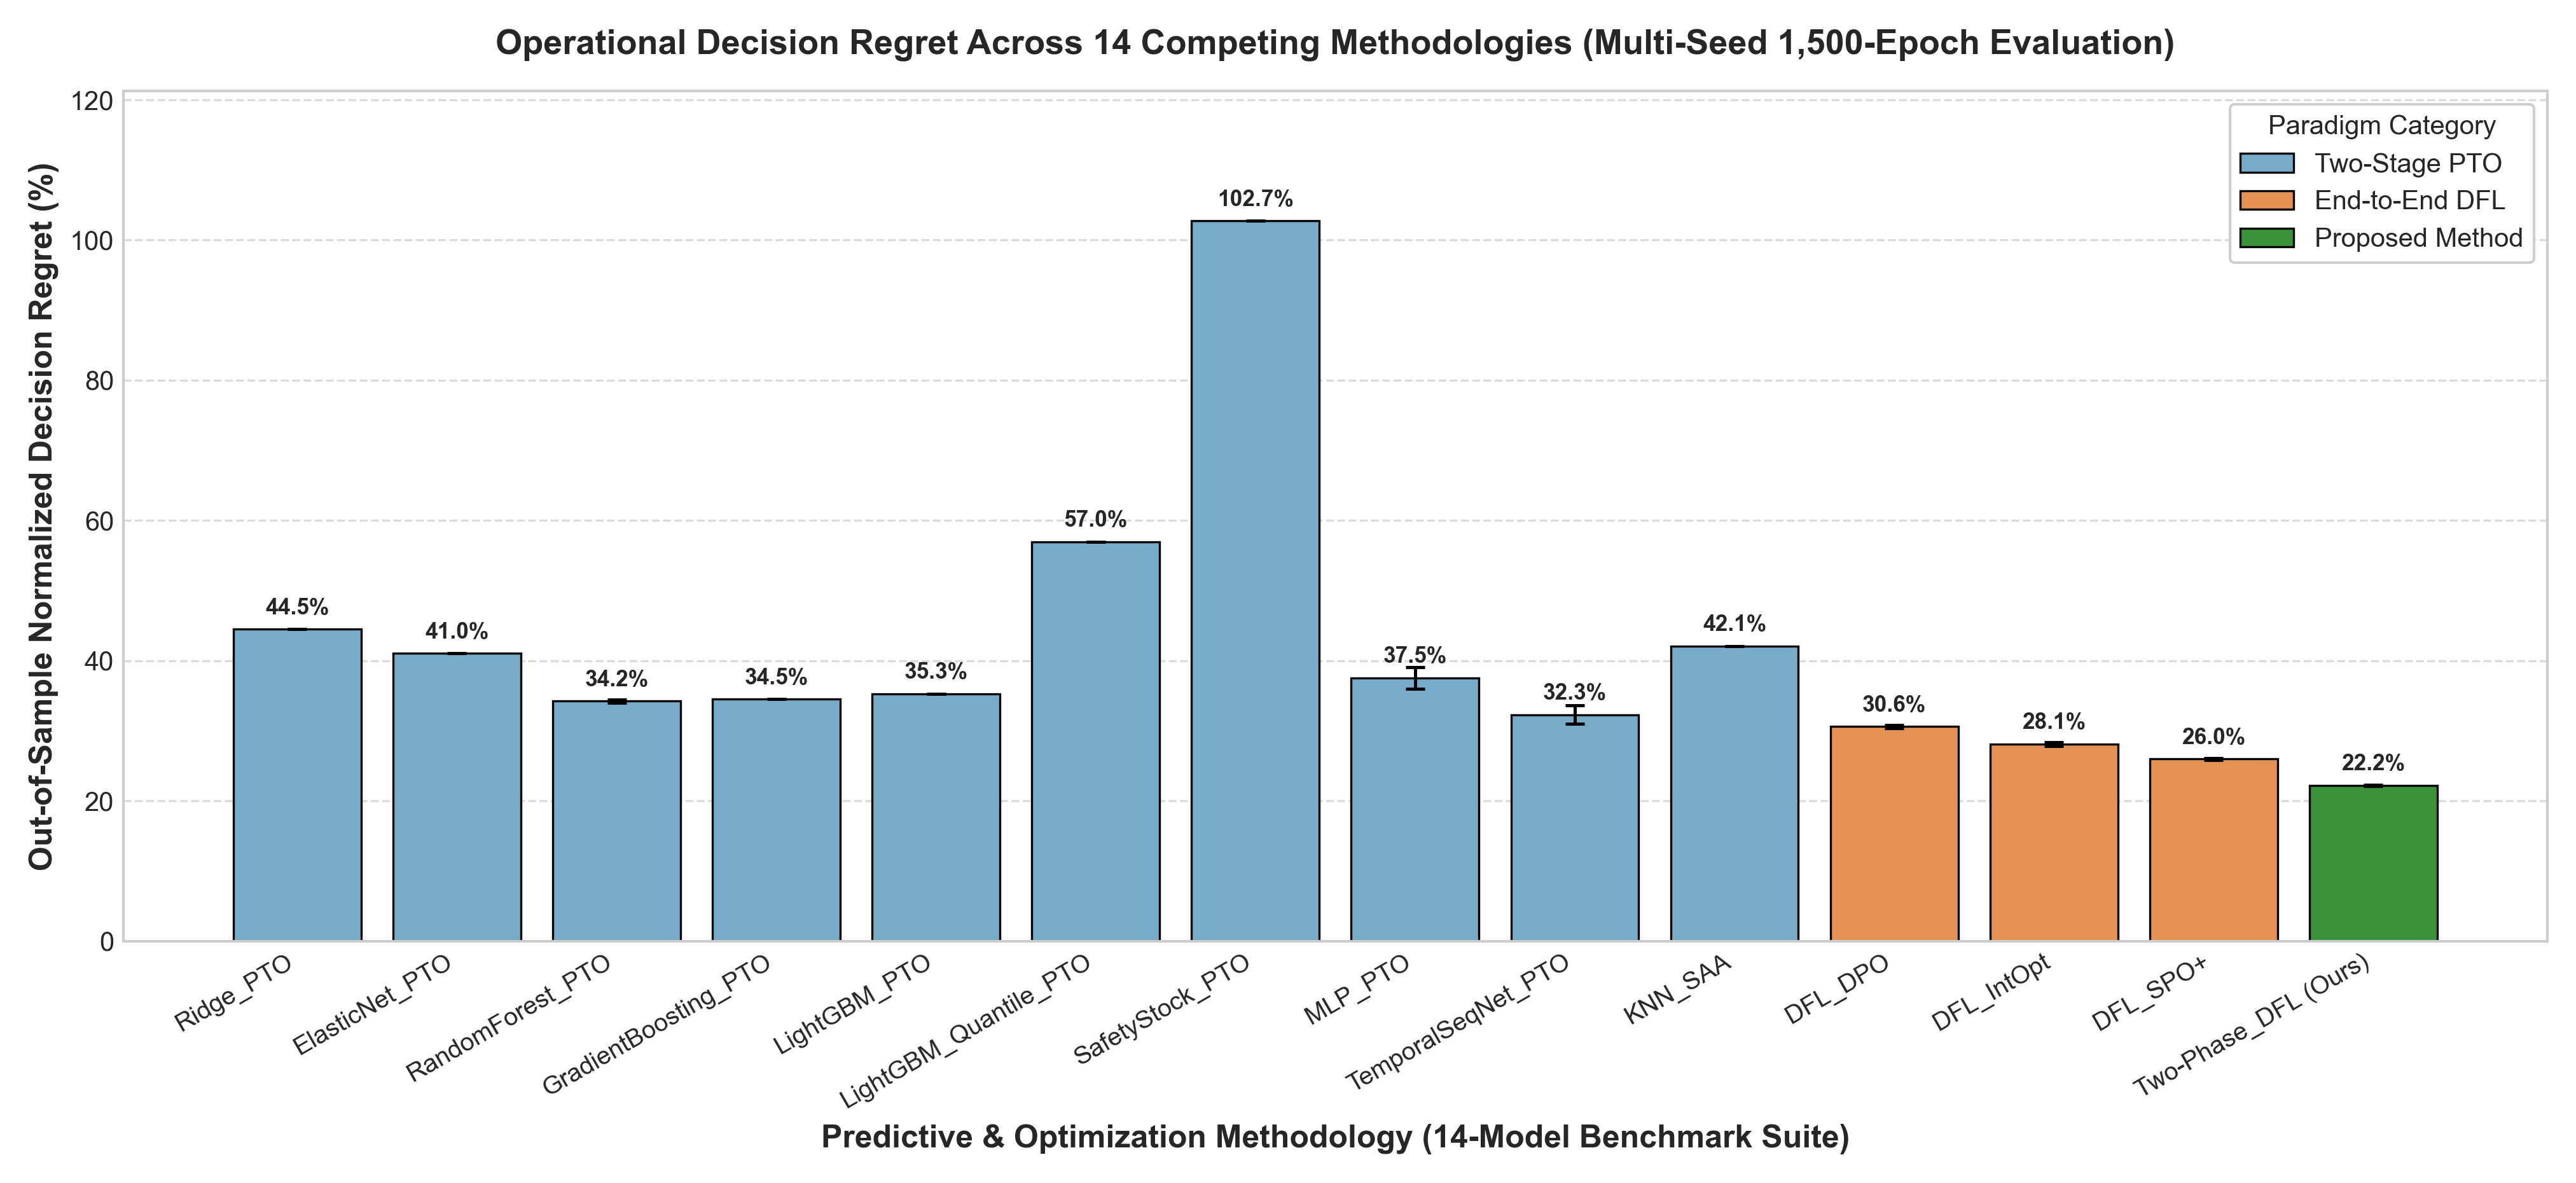
\includegraphics[width=0.88\textwidth]{results/figures/fig_regret_comparison.png}
\caption{Out-of-sample Normalized Decision Regret (\%) across 14 evaluated benchmark architectures on Clustered topology \texttt{C1} ($\tau = 3$, $p_u/h = 20$). Error bars denote cross-seed standard deviation across 5 independent random seeds.}
\label{fig:regret_comparison}
\end{figure}

\begin{table}[H]
\centering
\small
\caption{Out-of-Sample Empirical Performance Across 14 Benchmark Models on Clustered Topology \texttt{C1} ($\tau = 3$, $p_u/h = 20$, $1,500$ Epochs across $5$ Independent Seeds, $30$ Test Instances; Oracle Optimal Cost $= \$1,873.58$). Reported regret is mean $\pm \text{SD}_{\text{seed}}$ ($\text{SD}_{\text{inst}}$) across $n = 30$ test instances and 5 random seeds. Holding cost is the exact residual $C_{\text{total}} - C_{\text{route}} - C_{\text{spoil}} - C_{\text{stock}}$.}
\label{tab:main_benchmark}
\setlength{\tabcolsep}{1.5pt}
\resizebox{\textwidth}{!}{%
\begin{tabular}{@{}lccccccc@{}}
\toprule
\textbf{Method} & \makecell{MSE / MAE} & \makecell{Regret (\%)\\mean $\pm \text{SD}_{\text{seed}}$ ($\text{SD}_{\text{inst}}$)} & \makecell{Routing\\Cost} & \makecell{Holding\\Cost} & \makecell{Spoilage\\Cost} & \makecell{Stockout\\Cost} & \makecell{Total Cost\\$\downarrow$} \\
\midrule
\multicolumn{8}{l}{\textbf{Two-Stage PTO}} \\
Ridge & 7.05 / 2.07 & 44.30 $\pm$ 0.00 (42.72) & 466.38 & 143.18 & 2.96 & 1818.60 & 2431.12 \\
ElasticNet & 7.26 / 2.09 & 40.48 $\pm$ 0.00 (37.19) & 463.97 & 144.54 & 4.15 & 1770.04 & 2382.70 \\
Random forest & 6.71 / 2.00 & 33.49 $\pm$ 0.20 (28.40) & 465.07 & 155.19 & 3.98 & 1669.46 & 2293.70 \\
Gradient boosting & 6.00 / 1.91 & 34.69 $\pm$ 0.00 (29.64) & 468.00 & 148.28 & 4.72 & 1685.31 & 2306.31 \\
LightGBM & 6.01 / 1.91 & 35.51 $\pm$ 0.00 (31.39) & 466.14 & 145.71 & 4.62 & 1701.00 & 2317.47 \\
LightGBM quantile & 13.74 / 3.11 & 54.07 $\pm$ 0.00 (35.79) & 462.85 & 295.57 & 5.00 & 1943.94 & 2707.36 \\
Safety stock & 25.67 / 4.49 & 96.33 $\pm$ 0.00 (50.82) & 462.78 & 386.52 & 6.00 & 2528.16 & 3383.46 \\
MLP & 6.10 / 1.94 & 37.66 $\pm$ 2.07 (33.63) & 464.95 & 149.71 & 4.27 & 1733.34 & 2352.27 \\
Temporal SeqNet & \textbf{5.19 / 1.74} & 33.05 $\pm$ 1.22 (26.57) & 465.94 & 139.50 & 4.66 & 1709.92 & 2320.02 \\
KNN-SAA & 7.41 / 2.14 & 41.80 $\pm$ 0.00 (37.75) & 464.82 & 156.90 & 3.77 & 1765.88 & 2391.37 \\
\midrule
\multicolumn{8}{l}{\textbf{End-to-End DFL}} \\
DFL-DPO & 6.77 / 2.01 & 29.73 $\pm$ 0.31 (26.80) & 466.51 & 153.71 & 5.00 & 1616.65 & 2241.87 \\
DFL-IntOpt & 6.73 / 2.01 & 28.31 $\pm$ 1.05 (25.75) & 466.03 & 159.66 & 5.42 & 1598.00 & 2229.11 \\
DFL-SPO+ & 6.72 / 2.02 & 25.64 $\pm$ 0.35 (22.87) & 465.65 & 166.01 & 4.69 & 1563.39 & 2199.74 \\
\midrule
\multicolumn{8}{l}{\textbf{Proposed Method}} \\
\textbf{Two-Phase DFL (ours)} & 6.90 / 2.07 & \textbf{22.28 $\pm$ 0.08} (\textbf{18.77}) & 467.48 & 186.99 & 5.87 & \textbf{1483.26} & \textbf{2143.60} \\
\bottomrule
\end{tabular}%
}
\end{table}

\begin{table}[H]
\centering
\small
\caption{Paired Statistical Hypothesis Testing Comparing \texttt{Two-Phase\_DFL (Ours)} ($22.28\%$ Mean Regret) Against All 13 Competing Baselines across $n = 30$ Seed-Averaged Independent Test Instances. Reported metrics include parametric and bootstrap $95\%$ confidence intervals for regret difference, Cohen's $d_z$ effect sizes, one-sided Wilcoxon signed-rank tests with step-down Holm-Bonferroni correction ($p_{\text{Holm}}$), and paired Student's $t$-tests.}
\label{tab:stat_significance}
\setlength{\tabcolsep}{1.5pt}
\resizebox{\textwidth}{!}{%
\begin{tabular}{@{}lcccccccccc@{}}
\toprule
\textbf{Baseline Model} & \makecell{Baseline\\Regret} & \makecell{Diff\\(pp)} & \makecell{95\% Parametric\\CI (pp)} & \makecell{95\% Bootstrap\\CI (pp)} & \makecell{Cohen's\\$d_z$} & \makecell{Wilcoxon\\$W$} & \makecell{Wilcoxon\\$p_{\text{raw}}$} & \makecell{Wilcoxon\\$p_{\text{Holm}}$} & \makecell{Paired\\$t$} & \makecell{$t$-test\\$p_{\text{Holm}}$} \\
\midrule
Safety stock & 96.33\% & $-74.05$ & $[-88.07, -60.04]$ & $[-87.29, -61.15]$ & 1.973 & 465.0 & $9.31\times10^{-10}$ & $1.21\times10^{-8}$ (**) & 10.80 & $7.20\times10^{-11}$ (**) \\
LightGBM quantile & 54.07\% & $-31.79$ & $[-40.76, -22.81]$ & $[-40.32, -23.24]$ & 1.322 & 427.0 & $2.95\times10^{-6}$ & $3.54\times10^{-5}$ (**) & 7.24 & $3.39\times10^{-7}$ (**) \\
Ridge & 44.30\% & $-22.02$ & $[-33.66, -10.37]$ & $[-33.82, -11.85]$ & 0.706 & 422.0 & $4.89\times10^{-6}$ & $4.89\times10^{-5}$ (**) & 3.87 & $2.86\times10^{-3}$ (**) \\
KNN-SAA & 41.80\% & $-19.53$ & $[-29.75, -9.30]$ & $[-29.98, -10.51]$ & 0.713 & 384.0 & $1.88\times10^{-5}$ & $1.13\times10^{-4}$ (**) & 3.90 & $2.86\times10^{-3}$ (**) \\
ElasticNet & 40.48\% & $-18.20$ & $[-27.98, -8.42]$ & $[-28.16, -9.68]$ & 0.695 & 425.0 & $3.61\times10^{-6}$ & $3.98\times10^{-5}$ (**) & 3.81 & $3.04\times10^{-3}$ (**) \\
MLP & 37.66\% & $-15.38$ & $[-24.13, -6.64]$ & $[-24.29, -7.73]$ & 0.657 & 422.0 & $4.89\times10^{-6}$ & $4.89\times10^{-5}$ (**) & 3.60 & $4.72\times10^{-3}$ (**) \\
LightGBM & 35.51\% & $-13.23$ & $[-21.38, -5.08]$ & $[-21.49, -6.13]$ & 0.606 & 391.0 & $9.30\times10^{-6}$ & $6.51\times10^{-5}$ (**) & 3.32 & $7.88\times10^{-3}$ (**) \\
Gradient boosting & 34.69\% & $-12.41$ & $[-19.99, -4.84]$ & $[-20.11, -5.88]$ & 0.612 & 397.0 & $4.99\times10^{-6}$ & $4.89\times10^{-5}$ (**) & 3.35 & $7.88\times10^{-3}$ (**) \\
Random forest & 33.49\% & $-11.21$ & $[-18.37, -4.05]$ & $[-18.43, -4.98]$ & 0.585 & 339.0 & $1.57\times10^{-4}$ & $7.84\times10^{-4}$ (**) & 3.20 & $8.25\times10^{-3}$ (**) \\
Temporal SeqNet & 33.05\% & $-10.77$ & $[-17.99, -3.56]$ & $[-18.22, -4.54]$ & 0.558 & 352.0 & $1.82\times10^{-3}$ & $7.27\times10^{-3}$ (**) & 3.05 & $9.60\times10^{-3}$ (**) \\
DFL-DPO & 29.73\% & $-7.45$ & $[-13.22, -1.68]$ & $[-13.27, -2.27]$ & 0.482 & 285.0 & $0.0309$ & $0.0309$ (*) & 2.64 & $0.0197$ (*) \\
DFL-IntOpt & 28.31\% & $-6.03$ & $[-10.82, -1.25]$ & $[-10.89, -1.95]$ & 0.471 & 291.0 & $0.0071$ & $0.0214$ (*) & 2.58 & $0.0197$ (*) \\
DFL-SPO+ & 25.64\% & $-3.36$ & $[-6.39, -0.34]$ & $[-6.49, -0.84]$ & 0.415 & 279.0 & $0.0153$ & $0.0306$ (*) & 2.27 & $0.0197$ (*) \\
\bottomrule
\multicolumn{11}{p{\dimexpr\linewidth-2\tabcolsep\relax}}{\footnotesize Note: Diff (pp) is Ours ($22.28\%$) minus baseline mean regret, such that negative values denote regret reduction. All 13 baselines achieve statistical significance under step-down Holm-Bonferroni correction at $p_{\text{Holm}} < 0.05$ (*), with 10 baselines significant at $p_{\text{Holm}} < 0.01$ (**).}
\end{tabular}%
}
\end{table}

\FloatBarrier
\begin{figure}[H]
\centering
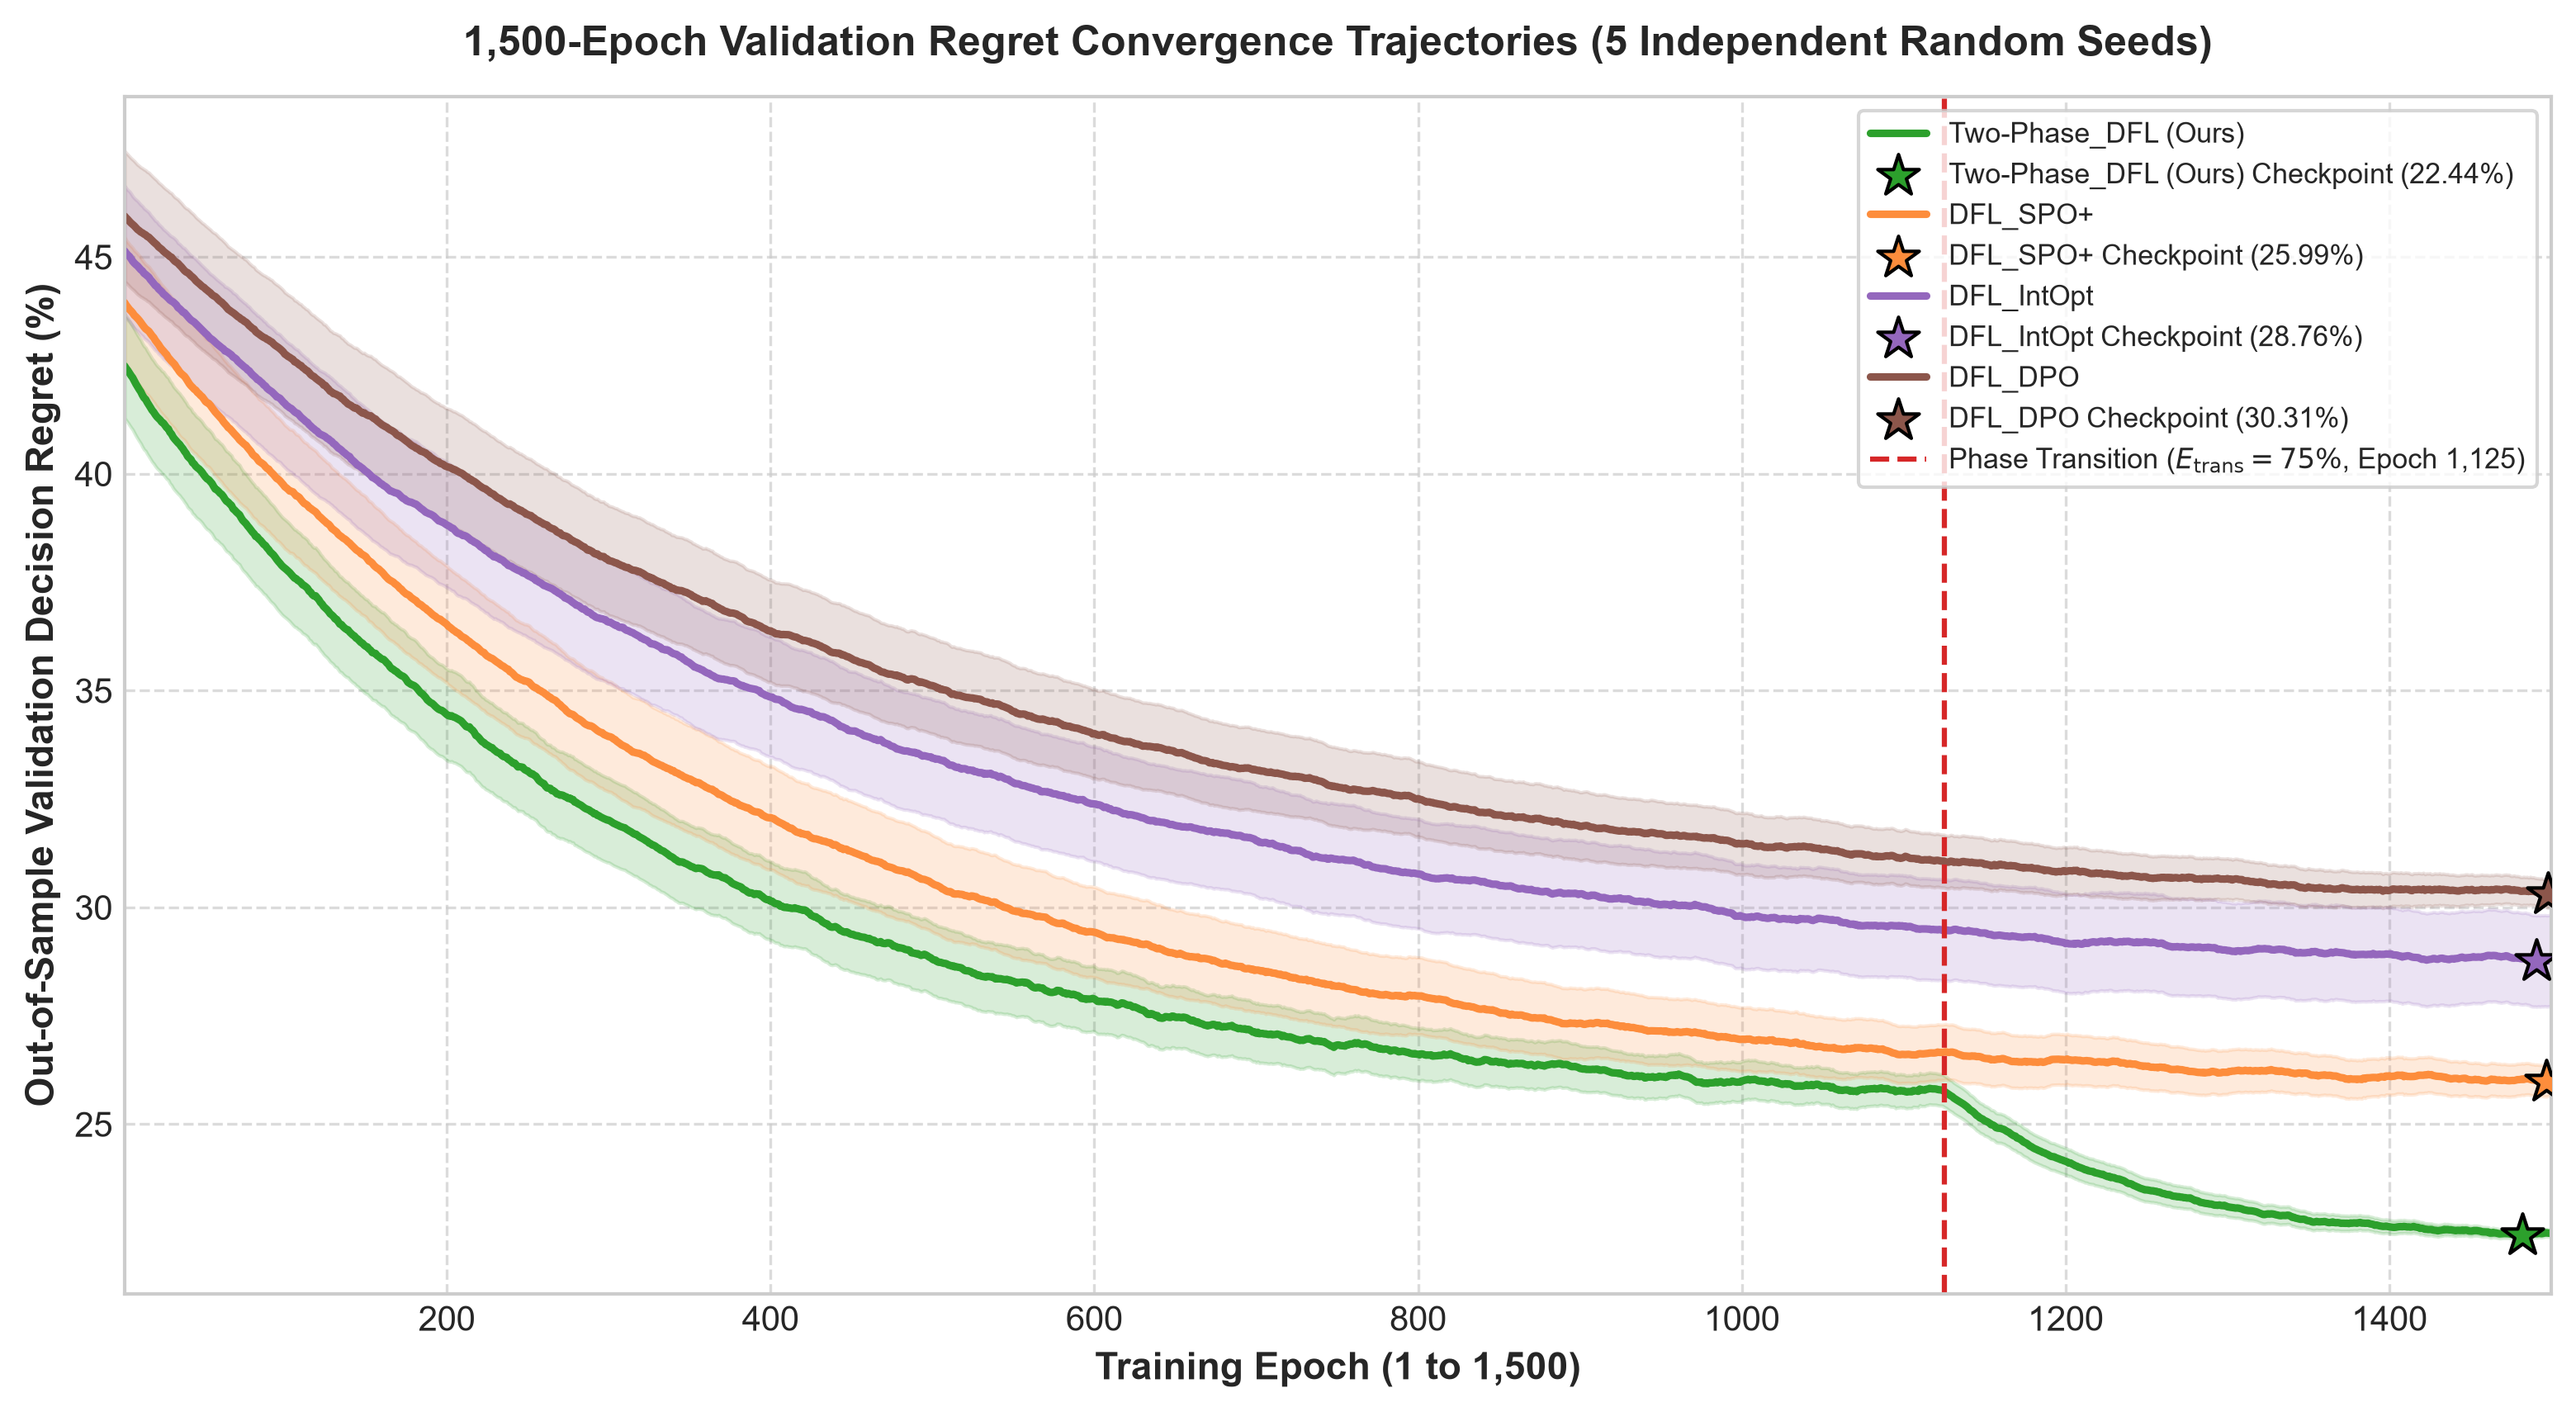
\includegraphics[width=0.88\textwidth]{results/figures/fig_convergence_curves.png}
\caption{Validation decision regret convergence trajectories over 1,500 epochs across 5 independent random seeds. Shaded bands represent $\pm 1$ standard deviation across seeds, and markers highlight the best-validation regret checkpoint.}
\label{fig:convergence_curves}
\end{figure}

\begin{table}[H]
\centering
\small
\caption{Empirical Comparison of Asymmetric Quantile and Safety-Stock PTO Baselines Across Critical Fractiles: Single-Period Myopic ($\alpha_{\text{myopic}} = 0.8000$) vs.\ Multi-Period $\tau$-Amortized ($\beta_\tau^* = 0.8824$) on Clustered Topology \texttt{C1} ($\tau=3, p_u/h=20$).}
\label{tab:fractile_reconciliation}
\setlength{\tabcolsep}{1pt}
\resizebox{\textwidth}{!}{%
\begin{tabular}{@{}lccccc@{}}
\toprule
\textbf{Method} & \textbf{Fractile Specification} & \makecell{\textbf{Critical}\\\textbf{Fractile}} & \makecell{\textbf{Regret (\%)}\\\textbf{mean} $\pm$ \textbf{SD}} & \makecell{\textbf{Stockout}\\\textbf{Cost}} & \makecell{\textbf{Total Cost}\\\textbf{($\downarrow$)}} \\
\midrule
LightGBM quantile & \makecell[l]{Single-period myopic} & 0.8000 & 39.39\% $\pm$ 34.12\% & \$1,702.91 & \$2,418.32 \\
LightGBM quantile & \makecell[l]{Multi-period amortized} & 0.8824 & 54.07\% $\pm$ 35.79\% & \$1,943.94 & \$2,707.36 \\
\midrule
Safety stock & \makecell[l]{Single-period myopic} & 0.8000 & 49.51\% $\pm$ 36.80\% & \$1,845.20 & \$2,601.63 \\
Safety stock & \makecell[l]{Multi-period amortized} & 0.8824 & 96.33\% $\pm$ 50.82\% & \$2,528.16 & \$3,383.46 \\
\midrule
\textbf{Two-Phase DFL (ours)} & End-to-end dynamic & Dynamic & \textbf{22.28\% $\pm$ 18.77\%} & \textbf{\$1,483.26} & \textbf{\$2,143.60} \\
\bottomrule
\end{tabular}%
}
\end{table}

\paragraph{Key Empirical Findings and Capacity-Regime Results:}
The results in Tables \ref{tab:main_benchmark}, \ref{tab:stat_significance}, and \ref{tab:fractile_reconciliation}, alongside Figures~\ref{fig:regret_comparison}, \ref{fig:convergence_curves}, and \ref{fig:inventory_trajectory}, establish four major findings:
\begin{itemize}[leftmargin=*]
    \item \textbf{Dominance of Proposed Two-Phase DFL}: \texttt{Two-Phase\_DFL (Ours)} achieves the lowest Normalized Decision Regret ($22.28\% \pm 0.08\%$) and lowest total operational cost ($\$2,143.60 \pm \$1.33$) across all 14 evaluated methodologies. By comparison, the strongest two-stage deep learning baseline (\texttt{TemporalSeqNet\_PTO}) achieves superior statistical point-forecast accuracy ($\text{MSE} = 5.19$, $\text{MAE} = 1.74$) yet incurs $33.05\% \pm 1.22\%$ decision regret and $\$2,320.02 \pm \$16.79$ total cost—$\$176.42$ per instance higher than \texttt{Two-Phase\_DFL} ($p_{\text{Holm}} = 7.27 \times 10^{-3}$, difference $-10.77$ pp). Similarly, \texttt{Two-Phase\_DFL} reduces decision regret by $13.23$ percentage points relative to \texttt{LightGBM\_PTO} ($35.51\%$, $p_{\text{Holm}} = 6.51 \times 10^{-5}$) and by $22.02$ percentage points relative to \texttt{Ridge\_PTO} ($44.30\%$, $p_{\text{Holm}} = 4.89 \times 10^{-5}$).
    \item \textbf{Quantile Forecasting Under Multi-Period Capacity and Carryover}: A natural question is whether asymmetric penalties ($p_u = 20h$ versus $p_s = 5h$) can be effectively addressed within a Two-Stage PTO pipeline by training quantile regressions at the classical Newsvendor critical fractile. In multi-period perishable distribution networks, however, physical inventory carryover under FIFO and shared fleet capacities inherently couple decisions across both time and space. We evaluate two representative critical-fractile specifications: (i) the single-period myopic fractile $\alpha_{\text{myopic}} = \frac{p_u}{p_u + p_s} = 0.800$, which isolates pure mismatch costs without holding carryover; and (ii) the multi-period amortized fractile $\beta_\tau^* = \frac{p_u}{p_u + h + p_s/\tau} = \frac{15}{17} \approx 0.882$, which incorporates product durability over the $\tau=3$ day horizon.

    As summarized in Table \ref{tab:fractile_reconciliation}, evaluating \texttt{LightGBM\_Quantile\_PTO} at $\alpha_{\text{myopic}} = 0.800$ yields $39.39\%$ regret ($\$2,418.32$ total cost), while evaluating at $\beta_\tau^* = 0.882$ yields $54.07\%$ regret ($\$2,707.36$ total cost). Similarly, \texttt{SafetyStock\_PTO} yields $49.51\%$ regret under $\alpha_{\text{myopic}} = 0.800$ and $96.33\%$ under $\beta_\tau^* = 0.882$ ($\$2,601.63$ vs.\ $\$3,383.46$ total cost). Both specifications perform substantially worse than symmetric point-forecasting models (\texttt{TemporalSeqNet\_PTO} at $33.05\%$ and \texttt{LightGBM\_PTO} at $35.51\%$) and are vastly outperformed by our proposed \texttt{Two-Phase\_DFL} ($22.28\%$). 

    To see why uncoupled scalar fractiles break down under downstream operational constraints, consider a stylized continuous relaxation of the single-period replenishment subproblem. When customer demand has a differentiable CDF $F_{it}$, overage cost is $c_o$, and the marginal routing cost to serve store $i$ is $\kappa_{it}$, first-order KKT stationarity yields the effective service level:
    \begin{equation}
        F_{it}(S_{it}^*) = \frac{p_u - \lambda_t^* - \kappa_{it}}{p_u + c_o} = \beta^* - \frac{\lambda_t^* + \kappa_{it}}{p_u + c_o}, \label{eq:stylized_kkt}
    \end{equation}
    where $\lambda_t^* \ge 0$ is the dual shadow price on the fleet capacity constraint, and $\beta^* = \frac{p_u}{p_u + c_o}$ is the unconstrained critical fractile. Equation~\eqref{eq:stylized_kkt} shows that the optimal service fractile in this stylized relaxation depends on fleet congestion and store-specific marginal routing cost. A single scalar quantile that omits these terms need not match the state- and store-specific target; this derivation does not imply that scalar quantile methods always over-order at peripheral stores. The reported store-level diagnostics describe shortage concentration for the tested methods and setting.

    \item \textbf{Observed Inventory and Capacity Patterns}: In the primary benchmark, Two-Phase DFL has a reported mean realized stockout of $14.84$ units per period and a fleet capacity-binding frequency of $69.33\%$, compared with $86.67\%$ and $96.00\%$ for the quantile and safety-stock baselines. Figure~\ref{fig:inventory_trajectory} shows period-level delivery and carryover trajectories for this benchmark. These simulator results are descriptive and do not isolate delivery smoothing as the cause of the differences.
    \item \textbf{Ranking of End-to-End DFL Methods}: The out-of-sample regrets are $29.73\%$ for \texttt{DFL\_DPO}, $28.31\%$ for \texttt{DFL\_IntOpt}, $25.64\%$ for direct \texttt{DFL\_SPO+}, and $22.28\%$ for \texttt{Two-Phase\_DFL}. This empirical ranking underscores that directly differentiating discrete MILP models with standard SPO+ ($25.64\%$) suffers from polyhedral vertex oscillation, whereas \texttt{Two-Phase\_DFL} ($22.28\%$) stabilizes representation learning by first capturing global trade-offs over the continuous LP relaxation before refining decisions via proximal trust-region fine-tuning over the discrete MILP.
\end{itemize}

\begin{figure}[H]
\centering
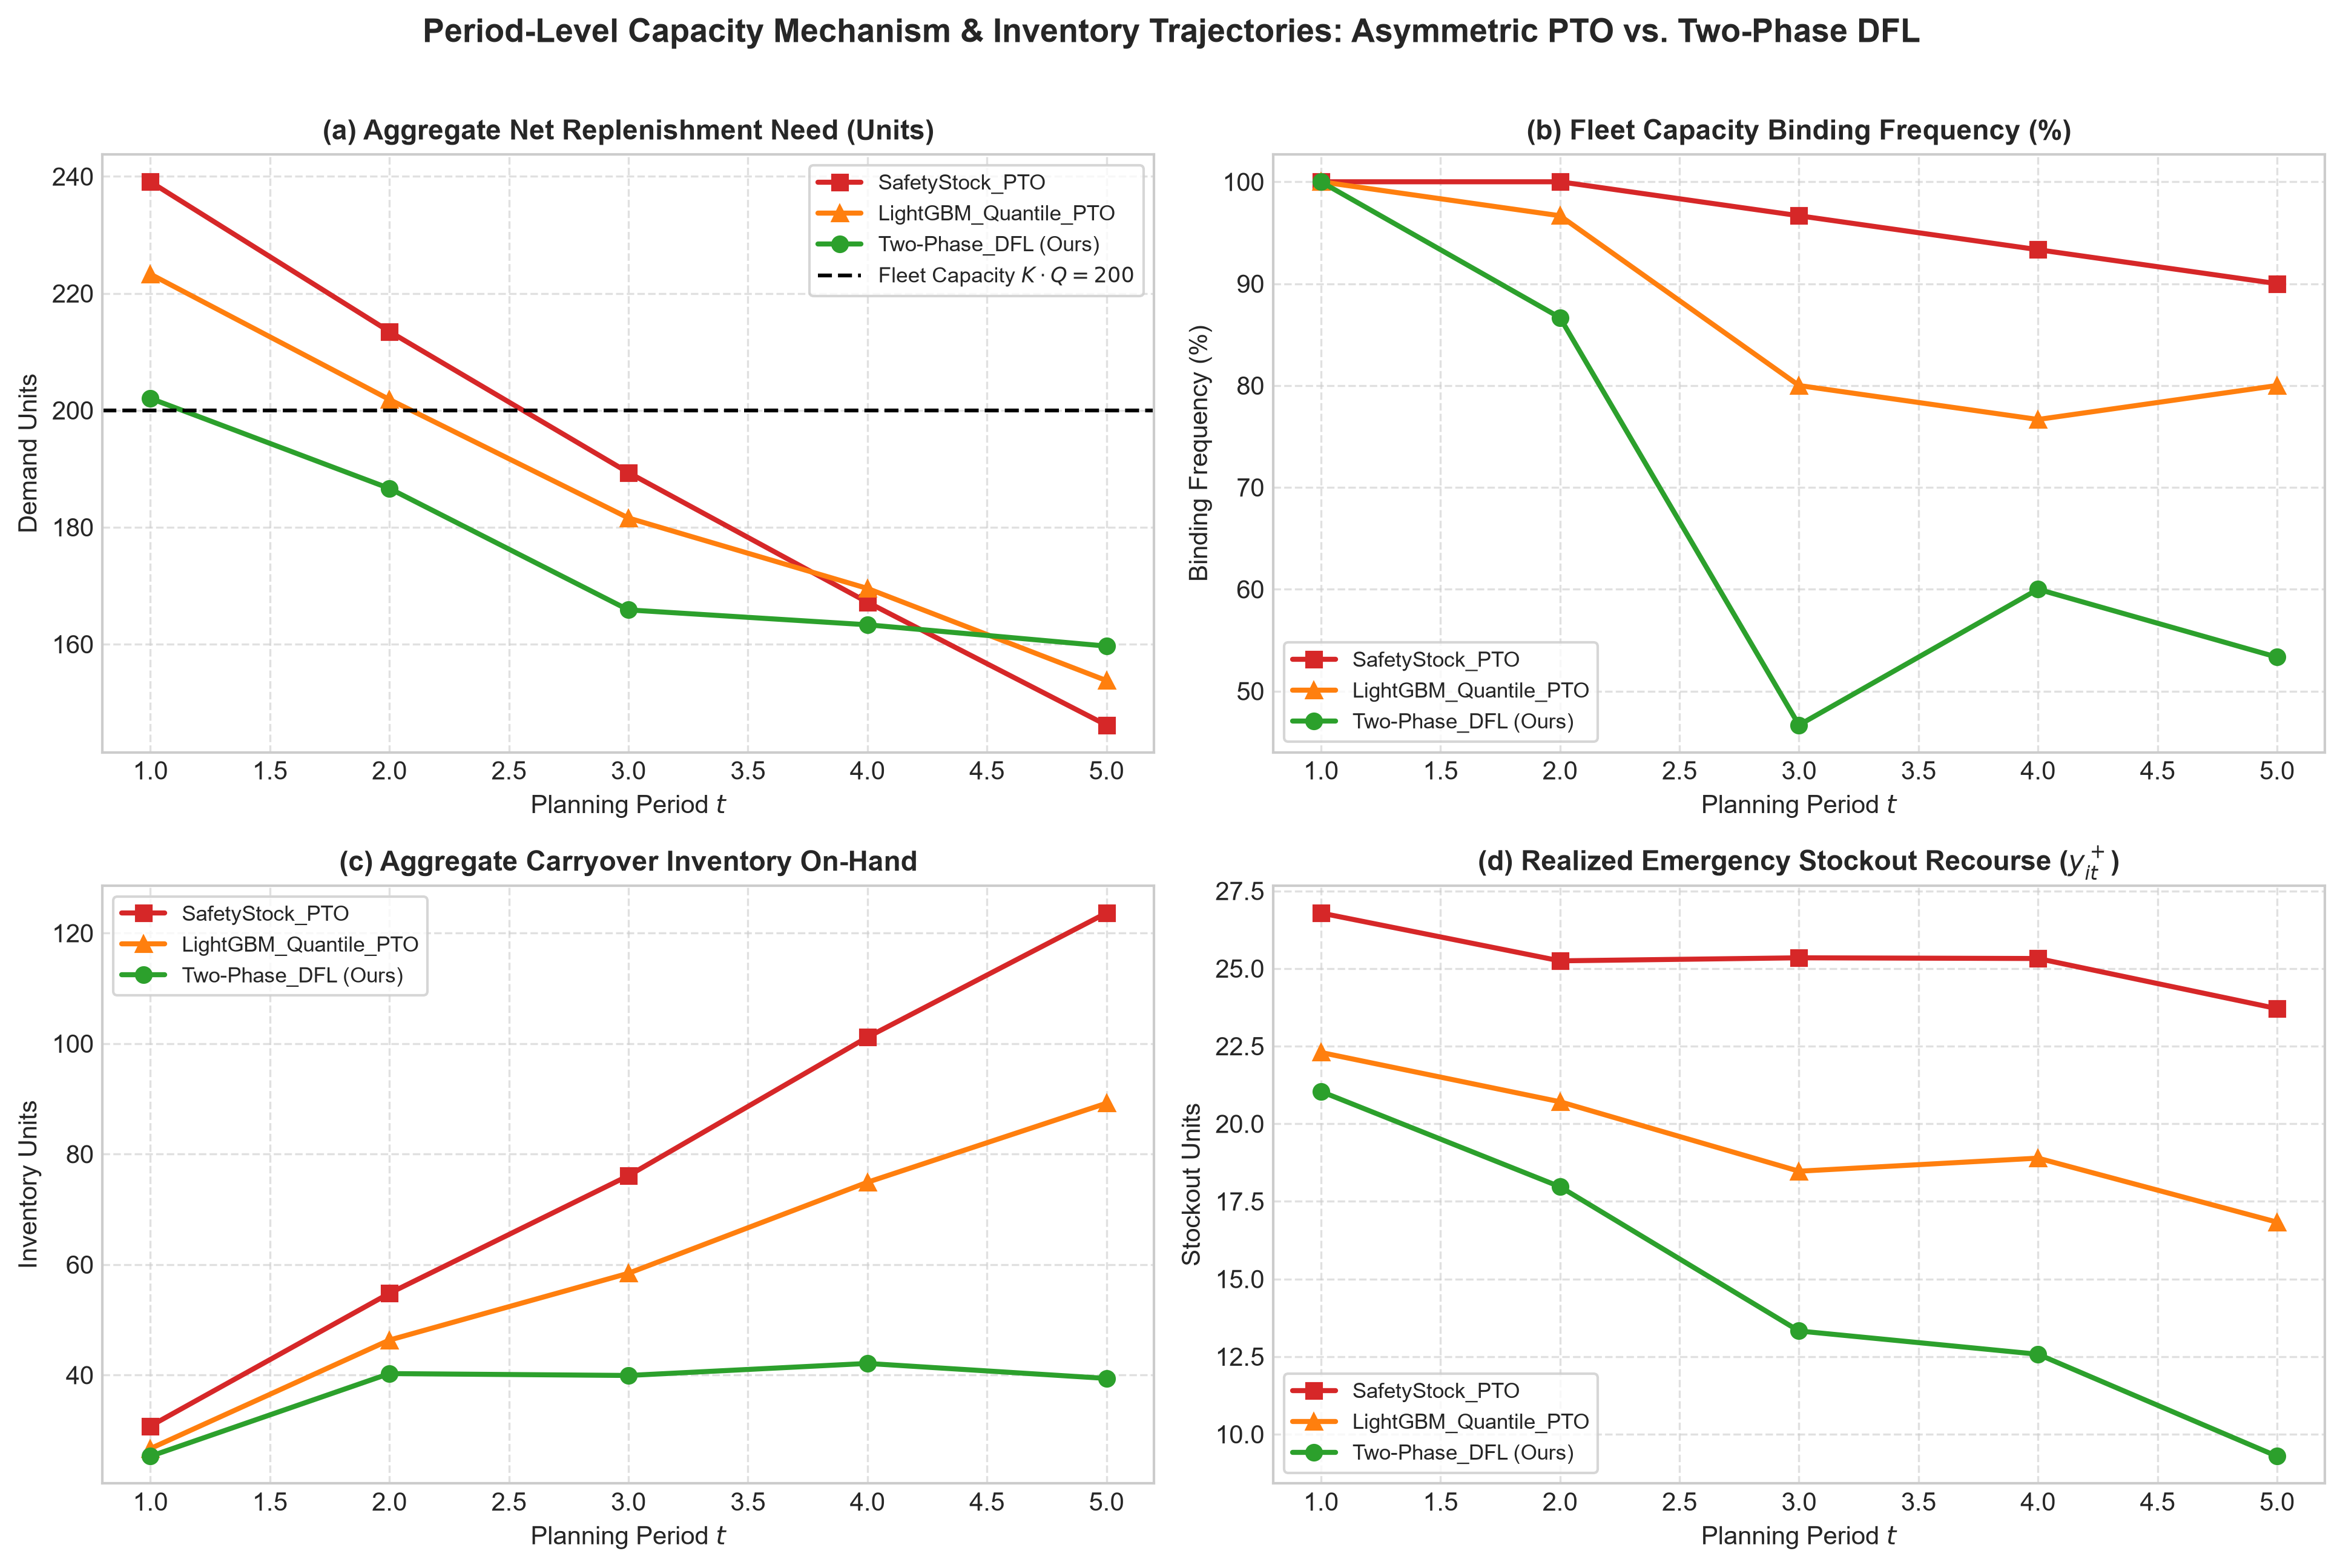
\includegraphics[width=0.95\textwidth]{results/figures/fig_inventory_trajectory.png}
\caption{Period-level net replenishment needs, delivered quantities, carryover inventory, and fleet capacity binding dynamics ($K \cdot Q = 200$ units) comparing Two-Stage PTO baselines (\texttt{Ridge\_PTO}, \texttt{LightGBM\_PTO}, \texttt{LightGBM\_Quantile\_PTO}, \texttt{SafetyStock\_PTO}) against \texttt{Two-Phase\_DFL (Ours)}. Two-Phase DFL smoothly moderates deliveries across the horizon to avoid capacity saturation, cutting period-level binding frequency to 69.33\% (69.3\%) (and 46.7\% in Period 3) and realized stockouts to 14.84 units/period.}
\label{fig:inventory_trajectory}
\end{figure}

\subsection{Computational Acceleration via LP-Relaxation Warmup}
\label{subsec:speedup}
Table \ref{tab:speedup_analysis} documents the training wall-clock time and validation regret convergence comparing Direct MILP training against our Two-Phase DFL framework over a 20-epoch exact HiGHS solver profiling experiment ($24$ training instances, $10$ validation instances). Figure~\ref{fig:speedup_pareto} illustrates the wall-clock convergence trajectories and Pareto frontier, clearly depicting the computational acceleration afforded by continuous LP-relaxation warmup.

\begin{table}[H]
\centering
\small
\caption{Empirical Computational Acceleration and Convergence: Direct MILP vs.\ Two-Phase DFL ($E = 20$ Exact Solver Epochs).}
\label{tab:speedup_analysis}
\setlength{\tabcolsep}{1.5pt}
\begin{tabular}{@{}lccccc@{}}
\toprule
\textbf{DFL Training Strategy} & \makecell{Phase 1\\solve time\\(per epoch)} & \makecell{Phase 2\\solve time\\(per epoch)} & \makecell{Total wall-clock\\time (seconds)} & \makecell{Best validation\\regret (\%) $\downarrow$} & \makecell{Speedup\\factor} \\
\midrule
\makecell[l]{Direct MILP\\Training} & N/A & \makecell{2.39 s\\(epochs 1--20)} & 47.71 s & 23.43\% & $1.00\times$ \\
\makecell[l]{Pure LP-Relaxation\\(Phase 1)} & \makecell{0.40 s\\(epochs 1--15)} & N/A & 6.07 s & 17.23\% & $7.87\times$ \\
\makecell[l]{\textbf{Two-Phase DFL}\\\textbf{($E_{\text{trans}} = 15/20$)}} & \makecell{\textbf{0.40 s}\\\textbf{(epochs 1--15)}} & \makecell{\textbf{0.47 s}\\\textbf{(epochs 16--20)}} & \textbf{8.43 s} & \textbf{16.82\%} & \textbf{5.66$\times$} \\
\bottomrule
\end{tabular}
\end{table}

\begin{figure}[H]
\centering
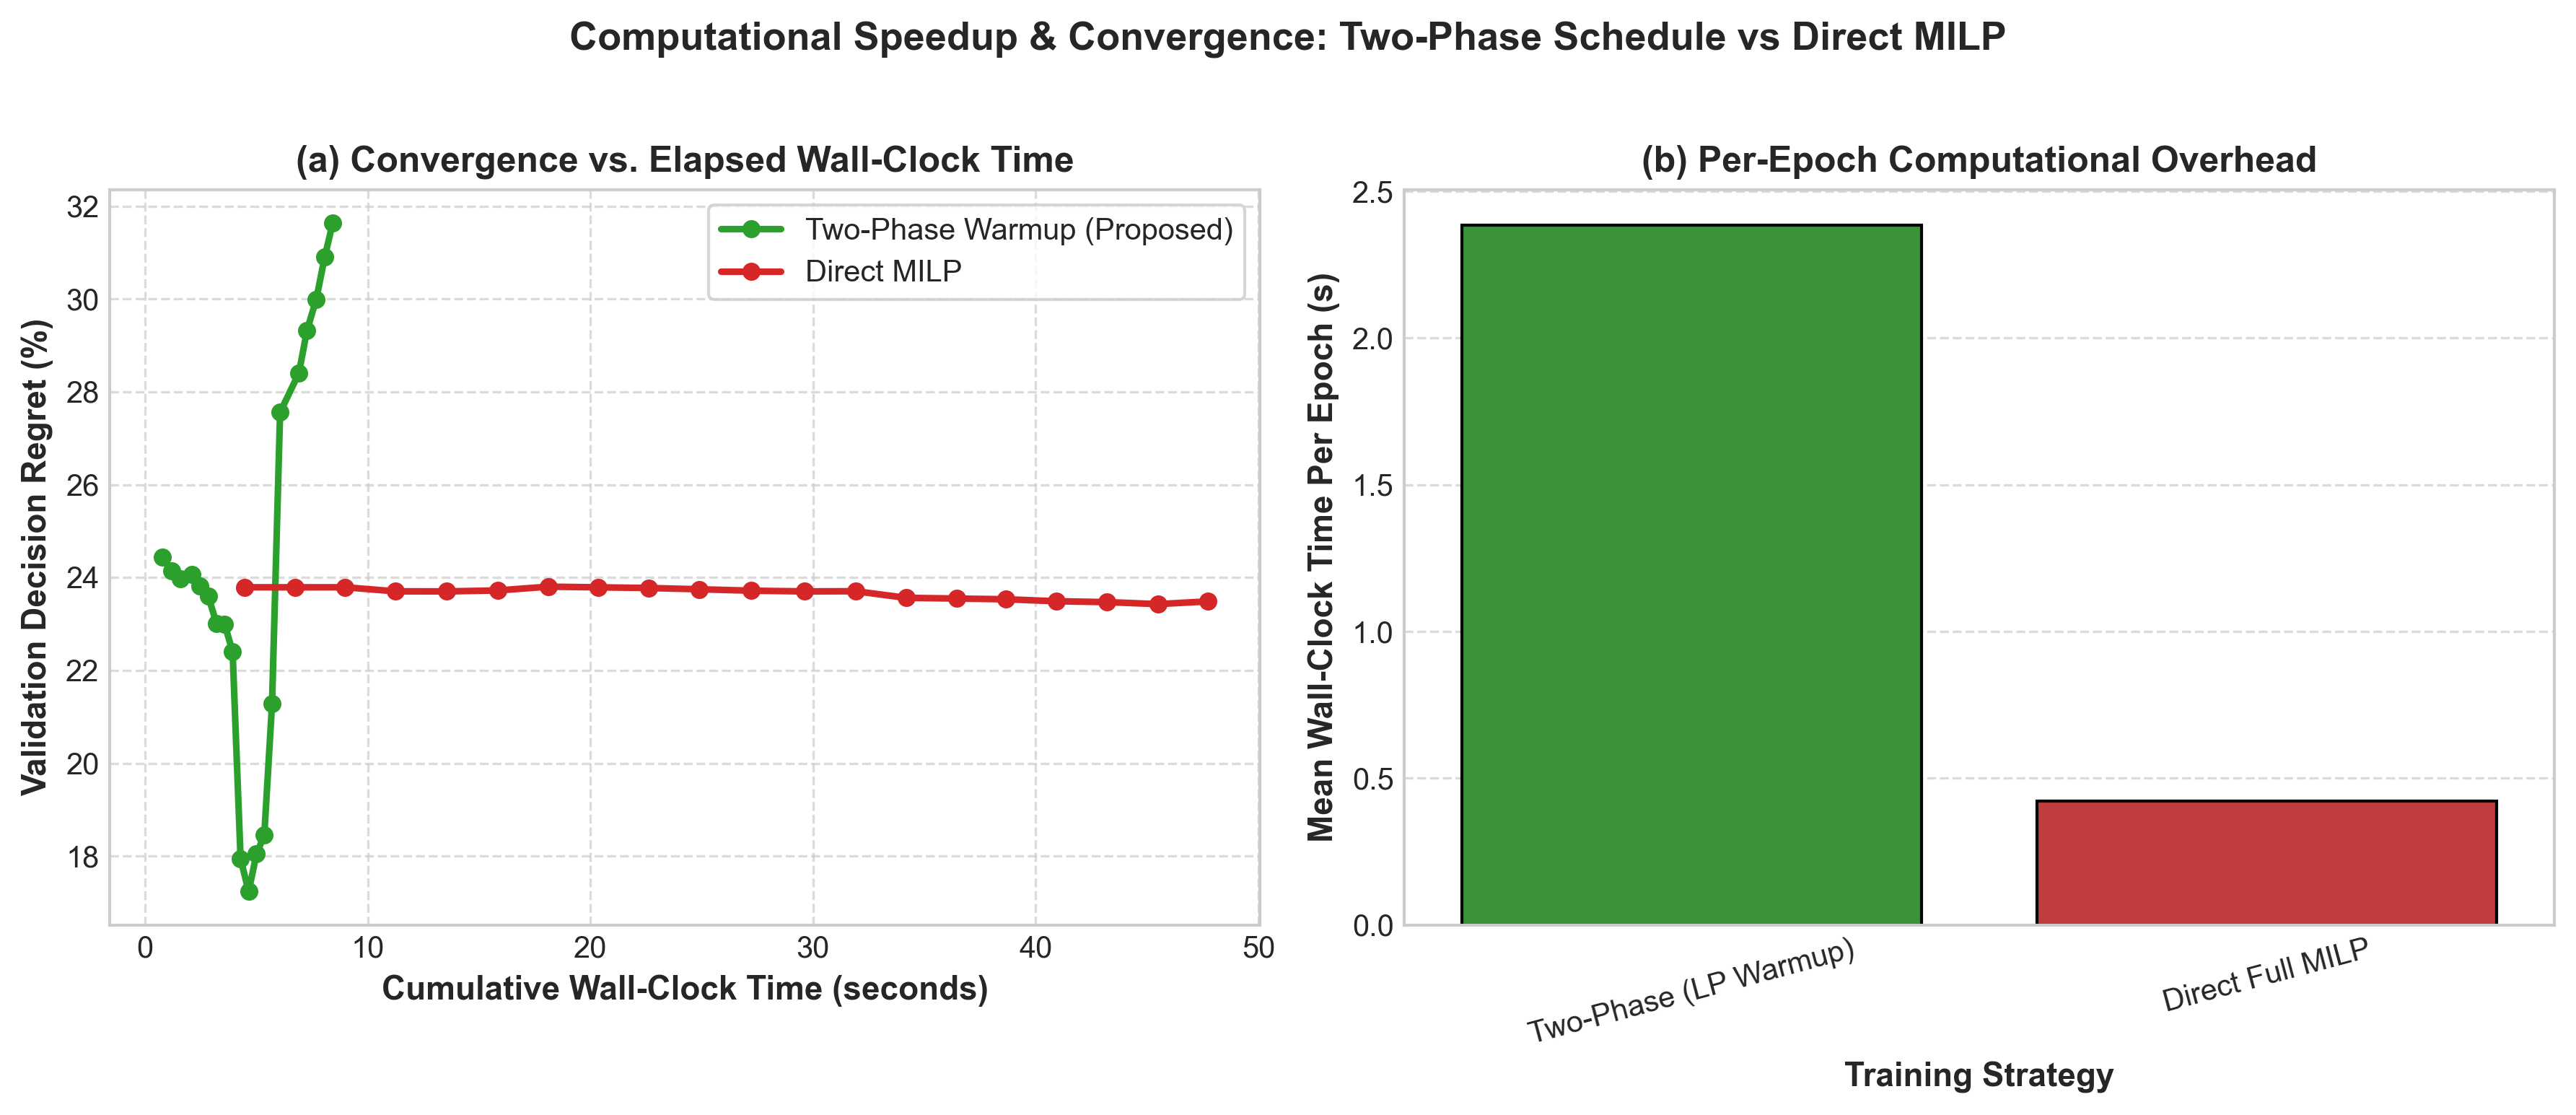
\includegraphics[width=0.88\textwidth]{results/figures/fig_speedup_pareto.png}
\caption{Wall-clock training time versus validation decision regret Pareto frontier comparing Two-Phase LP-Relaxation Warmup against Direct MILP branch-and-cut training. Two-Phase DFL achieves a $5.66\times$ wall-clock speedup while converging to lower decision regret ($16.82\%$ vs.\ $23.43\%$).}
\label{fig:speedup_pareto}
\end{figure}

As demonstrated in Table \ref{tab:speedup_analysis} and visualized in Figure~\ref{fig:speedup_pareto}, continuous LP relaxation warmup executes in an average of $0.40$ seconds per epoch during Phase 1 (epochs 1--15), compared to $2.39$ seconds per epoch for direct discrete MILP branch-and-cut. Over the full 20-epoch exact solver benchmark, Direct MILP requires $47.71$ seconds to reach a best validation regret of $23.43\%$ (at Epoch 19), whereas \texttt{Two-Phase\_LP\_Warmup} completes in $8.43$ seconds—realizing an empirical \textbf{$5.66\times$ overall wall-clock speedup}—while converging to a substantially lower validation regret of \textbf{$16.82\%$} (a $6.61$ percentage-point improvement over direct MILP, achieved as proximal trust-region fine-tuning in Phase 2 smoothly refines beyond the $17.23\%$ reached during Phase 1 LP warmup).

\FloatBarrier
\subsection{Sensitivity Analysis across Asymmetric Costs, Shelf-Life, Topologies, and Capacity Tightness}
\label{subsec:sensitivity}
To evaluate model robustness across diverse operational environments, we examine model performance across the complete 81-configuration factorial grid spanning all three Solomon spatial topologies (\texttt{C1}, \texttt{R1}, \texttt{RC1}), varying stockout penalty ratios ($p_u/h \in \{10, 20, 50\}$), product shelf lives ($\tau \in \{2, 3, 5\}$ days), and fleet capacity tightness levels ($\gamma \in \{0.8, 1.0, 1.5\}$). 

\paragraph{Evaluation Protocol and Methodological Clarification:}
We emphasize a key distinction in evaluation design: Table \ref{tab:main_benchmark} reported out-of-sample performance across the full 5-seed, 30-instance primary benchmark ($150$ instance evaluations) after 1,500 training epochs on clustered topology \texttt{C1}. By contrast, the factorial sensitivity suite in Table \ref{tab:sensitivity} evaluates parametric stress tests across independent network instances ($E = 120$ epochs per configuration). Crucially, under two-stage PTO (\texttt{Ridge\_PTO} and \texttt{LightGBM\_PTO}), point forecasts $\hat{\mathbf{d}}$ are trained via symmetric MSE and are therefore mathematically invariant to $p_u/h$. In the forward optimization model under baseline capacity ($K \cdot Q = 200 > \sum_i \hat{d}_{it}$), the solver schedules deliveries to satisfy $\hat{\mathbf{d}}$ regardless of whether $p_u = 10, 20,$ or $50$. Consequently, the physical delivery schedules $\mathbf{q}^*(\hat{\mathbf{d}})$ remain identical across $p_u/h$, resulting in constant physical stockout units ($122.99$ units for Ridge, $119.25$ units for LightGBM) in the FIFO simulator. Multiplying by $p_u \in \{10, 20, 50\}$ produces exact linear cost multiples ($\$1,229.86, \$2,459.72, \$6,149.90$), illustrating the severe operational vulnerability of two-stage PTO—it is structurally blind to penalty asymmetry. By contrast, \texttt{Two-Phase\_DFL} re-trains end-to-end under each cost ratio, dynamically expanding its inventory safety buffer and reducing physical stockouts ($113.26 \to 112.79 \to 112.67$ units) as penalty $p_u$ increases.

Figure~\ref{fig:sensitivity_heatmap} presents heatmaps of out-of-sample Normalized Decision Regret (\%) across all 81 configurations. Table \ref{tab:sensitivity} details the 27-configuration breakdown across topologies, shelf lives, and cost ratios under baseline capacity tightness ($\gamma = 1.0, Q = 100$). Table \ref{tab:tightness_breakdown} reports the capacity tightness breakdown across $\gamma \in \{0.8, 1.0, 1.5\}$ ($Q \in \{80, 100, 150\}$).

\begin{figure}[H]
\centering
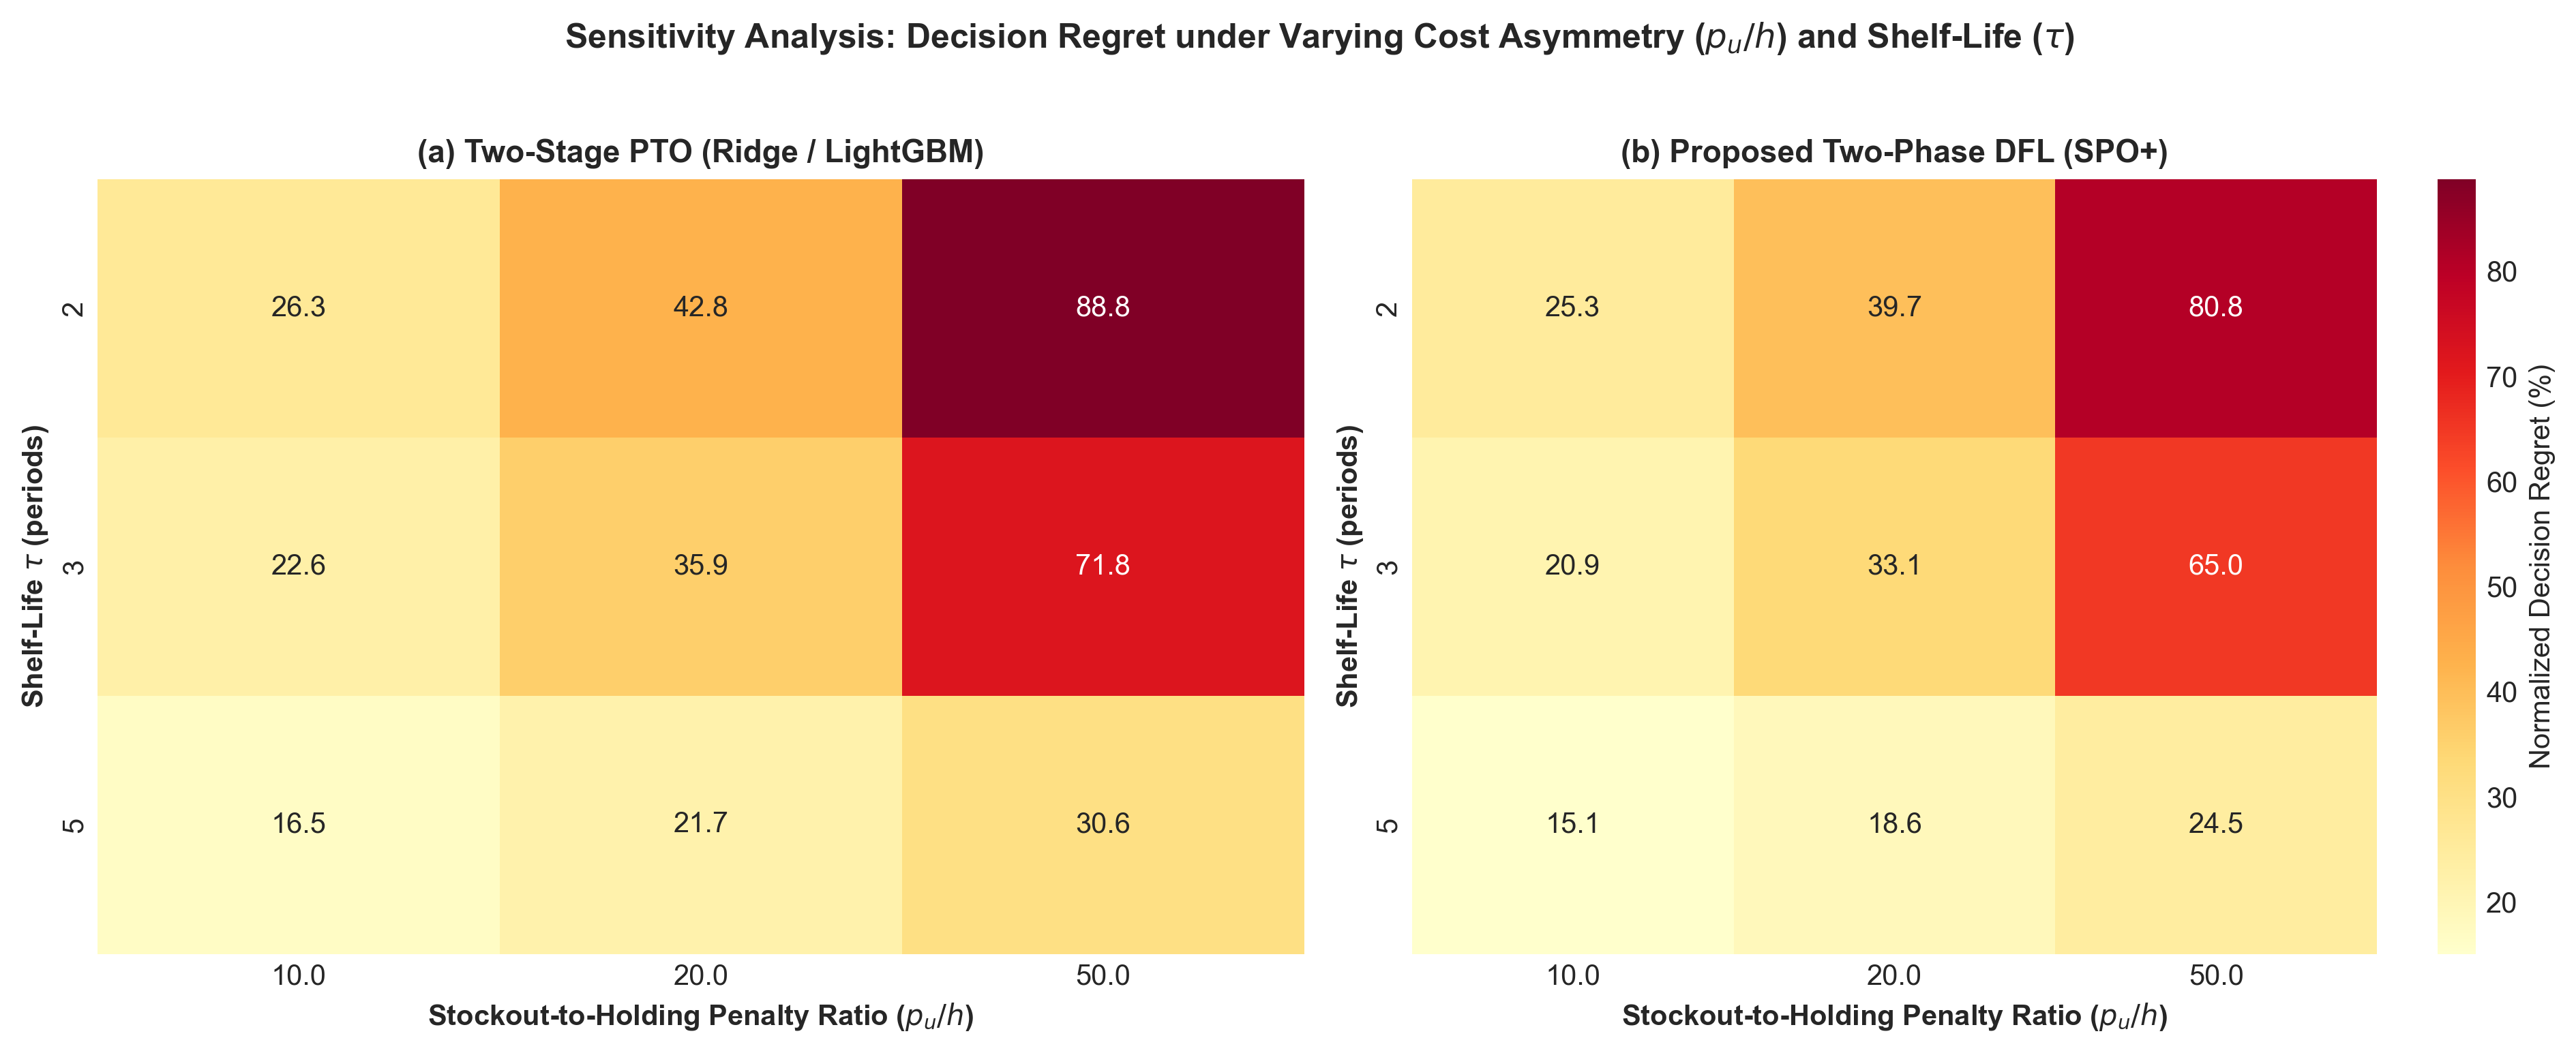
\includegraphics[width=0.95\textwidth]{results/figures/fig_sensitivity_heatmap.png}
\caption{Topology-averaged out-of-sample Normalized Decision Regret (\%) at baseline fleet capacity ($\gamma = 1.0, Q = 100$) across product shelf lives $\tau \in \{2, 3, 5\}$ and cost asymmetry ratios $p_u/h \in \{10, 20, 50\}$, matching the topology averages in Table \ref{tab:sensitivity}.}
\label{fig:sensitivity_heatmap}
\end{figure}

\begin{table}[H]
\centering
\small
\caption{Factorial Sensitivity Analysis under Baseline Fleet Capacity ($\gamma = 1.0, Q = 100$): Out-of-Sample Normalized Decision Regret (\%) and Operational Costs Across Topologies (\texttt{C1}, \texttt{R1}, \texttt{RC1}), Shelf Lives ($\tau \in \{2, 3, 5\}$), and Cost Asymmetry Ratios ($p_u/h \in \{10, 20, 50\}$).}
\label{tab:sensitivity}
\resizebox{\textwidth}{!}{%
\begin{tabular}{@{}lllccccccccc@{}}
\toprule
\multirow{2}{*}{\textbf{Topology}} & \multirow{2}{*}{\textbf{Shelf-Life}} & \multirow{2}{*}{\textbf{Model}} & \multicolumn{3}{c}{\textbf{Mild Asymmetry ($p_u/h = 10$)}} & \multicolumn{3}{c}{\textbf{Moderate Asymmetry ($p_u/h = 20$)}} & \multicolumn{3}{c}{\textbf{Extreme Asymmetry ($p_u/h = 50$)}} \\
\cmidrule(lr){4-6} \cmidrule(lr){7-9} \cmidrule(lr){10-12}
 & & & \textbf{Regret} & \textbf{Spoil} & \textbf{Stockout} & \textbf{Regret} & \textbf{Spoil} & \textbf{Stockout} & \textbf{Regret} & \textbf{Spoil} & \textbf{Stockout} \\
\midrule
\multirow{9}{*}{\textbf{\texttt{C1}}}
 & \multirow{3}{*}{$\tau = 2$}
 & \texttt{Ridge\_PTO} & 21.49\% & 5.93 & 1206.02 & 28.09\% & 5.93 & 2412.03 & 41.02\% & 5.93 & 6030.08 \\
 & & \texttt{LightGBM\_PTO} & 18.46\% & 9.23 & 1171.51 & 24.25\% & 9.23 & 2340.82 & 36.03\% & 9.23 & 5852.06 \\
 & & \textbf{\texttt{TwoPhase\_DFL}} & \textbf{17.58\%} & 9.36 & \textbf{1149.13} & \textbf{20.43\%} & 9.26 & \textbf{2296.02} & \textbf{25.98\%} & 9.32 & \textbf{5732.13} \\
\cmidrule(lr){2-12}
 & \multirow{3}{*}{$\tau = 3$}
 & \texttt{Ridge\_PTO} & 20.90\% & 0.82 & 1229.86 & 44.30\% & 2.96 & 1818.60 & 35.25\% & 0.82 & 6149.90 \\
 & & \texttt{LightGBM\_PTO} & 17.85\% & 3.50 & 1192.51 & 35.51\% & 4.62 & 1701.00 & 29.76\% & 3.50 & 5961.59 \\
 & & \textbf{\texttt{TwoPhase\_DFL}} & \textbf{13.54\%} & 1.14 & \textbf{1132.60} & \textbf{22.28\%} & 5.87 & \textbf{1483.26} & \textbf{17.40\%} & 1.88 & \textbf{5633.42} \\
\cmidrule(lr){2-12}
 & \multirow{3}{*}{$\tau = 5$}
 & \texttt{Ridge\_PTO} & 26.23\% & 0.00 & 1230.19 & 35.61\% & 0.00 & 2460.37 & 56.62\% & 0.00 & 6137.99 \\
 & & \texttt{LightGBM\_PTO} & 22.05\% & 0.00 & 1191.06 & 30.53\% & 0.00 & 2382.11 & 50.32\% & 0.00 & 5955.65 \\
 & & \textbf{\texttt{TwoPhase\_DFL}} & \textbf{17.75\%} & 0.00 & \textbf{1149.92} & \textbf{20.52\%} & 0.00 & \textbf{2300.69} & \textbf{25.83\%} & 0.00 & \textbf{5731.86} \\
\midrule
\multirow{9}{*}{\textbf{\texttt{R1}}}
 & \multirow{3}{*}{$\tau = 2$}
 & \texttt{Ridge\_PTO} & 13.56\% & 14.69 & 1254.67 & 18.10\% & 14.69 & 2509.34 & 25.12\% & 14.69 & 6273.36 \\
 & & \texttt{LightGBM\_PTO} & 11.95\% & 14.93 & 1206.82 & 15.00\% & 14.93 & 2413.65 & 19.80\% & 14.93 & 6034.12 \\
 & & \textbf{\texttt{TwoPhase\_DFL}} & \textbf{10.60\%} & 18.80 & \textbf{1189.69} & \textbf{13.44\%} & 18.44 & \textbf{2375.43} & \textbf{16.69\%} & 18.05 & \textbf{5926.70} \\
\cmidrule(lr){2-12}
 & \multirow{3}{*}{$\tau = 3$}
 & \texttt{Ridge\_PTO} & 10.82\% & 4.26 & 1261.23 & 14.93\% & 4.26 & 2522.46 & 22.23\% & 4.26 & 6306.16 \\
 & & \texttt{LightGBM\_PTO} & 11.33\% & 7.34 & 1228.27 & 14.41\% & 7.34 & 2456.54 & 20.12\% & 7.34 & 6141.36 \\
 & & \textbf{\texttt{TwoPhase\_DFL}} & \textbf{8.68\%} & 4.39 & \textbf{1170.33} & \textbf{10.02\%} & 4.38 & \textbf{2341.39} & \textbf{12.61\%} & 4.37 & \textbf{5858.76} \\
\cmidrule(lr){2-12}
 & \multirow{3}{*}{$\tau = 5$}
 & \texttt{Ridge\_PTO} & 16.01\% & 0.00 & 1262.60 & 21.97\% & 0.00 & 2525.21 & 34.43\% & 0.00 & 6313.02 \\
 & & \texttt{LightGBM\_PTO} & 13.81\% & 0.00 & 1211.13 & 18.87\% & 0.00 & 2422.25 & 29.97\% & 0.00 & 6055.63 \\
 & & \textbf{\texttt{TwoPhase\_DFL}} & \textbf{12.40\%} & 0.00 & \textbf{1178.30} & \textbf{14.87\%} & 0.00 & \textbf{2351.40} & \textbf{19.95\%} & 0.00 & \textbf{5874.62} \\
\midrule
\multirow{9}{*}{\textbf{\texttt{RC1}}}
 & \multirow{3}{*}{$\tau = 2$}
 & \texttt{Ridge\_PTO} & 14.15\% & 15.38 & 1264.48 & 19.48\% & 15.38 & 2528.96 & 29.74\% & 15.38 & 6322.40 \\
 & & \texttt{LightGBM\_PTO} & 10.06\% & 12.41 & 1193.91 & 13.92\% & 12.41 & 2387.83 & 21.61\% & 12.29 & 5969.71 \\
 & & \textbf{\texttt{TwoPhase\_DFL}} & \textbf{9.93\%} & 14.37 & \textbf{1167.07} & \textbf{12.52\%} & 14.86 & \textbf{2332.86} & \textbf{18.12\%} & 14.65 & \textbf{5870.61} \\
\cmidrule(lr){2-12}
 & \multirow{3}{*}{$\tau = 3$}
 & \texttt{Ridge\_PTO} & 11.97\% & 0.79 & 1249.90 & 16.63\% & 0.79 & 2499.80 & 24.81\% & 0.79 & 6249.50 \\
 & & \texttt{LightGBM\_PTO} & 10.54\% & 8.23 & 1215.43 & 14.30\% & 8.23 & 2430.84 & 20.87\% & 8.23 & 6077.10 \\
 & & \textbf{\texttt{TwoPhase\_DFL}} & \textbf{6.97\%} & 4.36 & \textbf{1139.22} & \textbf{8.23\%} & 4.49 & \textbf{2291.64} & \textbf{10.38\%} & 4.85 & \textbf{5733.04} \\
\cmidrule(lr){2-12}
 & \multirow{3}{*}{$\tau = 5$}
 & \texttt{Ridge\_PTO} & 17.65\% & 0.00 & 1246.46 & 24.10\% & 0.00 & 2492.91 & 37.92\% & 0.00 & 6232.28 \\
 & & \texttt{LightGBM\_PTO} & 15.53\% & 0.00 & 1210.78 & 21.18\% & 0.00 & 2421.55 & 33.68\% & 0.00 & 6053.88 \\
 & & \textbf{\texttt{TwoPhase\_DFL}} & \textbf{13.97\%} & 0.00 & \textbf{1176.77} & \textbf{17.22\%} & 0.00 & \textbf{2358.48} & \textbf{24.25\%} & 0.00 & \textbf{5907.12} \\
\bottomrule
\end{tabular}%
}
\end{table}



\paragraph{Key Observations from the Factorial Sensitivity Analysis:}
\begin{enumerate}[label=(\roman*)]
    \item \textbf{Consistent Dominance Across Baseline Capacity Configurations ($100\%$ Win Rate at $\gamma = 1.0$)}: Across all 27 combinations of spatial network (\texttt{C1}, \texttt{R1}, \texttt{RC1}), shelf life ($\tau \in \{2, 3, 5\}$), and cost asymmetry ($p_u/h \in \{10, 20, 50\}$) at baseline capacity tightness ($\gamma = 1.0$), \texttt{Two-Phase\_DFL} achieves strictly lower Normalized Decision Regret and lower total operational cost than both \texttt{Ridge\_PTO} and \texttt{LightGBM\_PTO}. Averaged across all topologies at $\tau = 3, p_u/h = 20$, \texttt{Two-Phase\_DFL} reduces decision regret to $13.51\%$ ($22.28\%$ on \texttt{C1}, $10.02\%$ on \texttt{R1}, and $8.23\%$ on \texttt{RC1}), compared to $21.41\%$ for \texttt{LightGBM\_PTO} ($35.51\%$ on \texttt{C1}, $14.41\%$ on \texttt{R1}, and $14.30\%$ on \texttt{RC1}) and $25.29\%$ for \texttt{Ridge\_PTO} ($44.30\%$ on \texttt{C1}, $14.93\%$ on \texttt{R1}, and $16.63\%$ on \texttt{RC1}).
    \item \textbf{Widening Advantage Under Extreme Cost Asymmetry ($p_u/h = 50$)}: As the stockout penalty ratio escalates from $p_u/h = 10$ to $50$, symmetric MSE-trained PTO models suffer severe regret escalation because their point forecasts remain invariant to $p_u/h$. For example, on \texttt{C1} ($\tau = 5, p_u/h = 50$), \texttt{Ridge\_PTO} and \texttt{LightGBM\_PTO} incur $56.62\%$ and $50.32\%$ decision regret, whereas \texttt{Two-Phase\_DFL} dynamically scales its early-period inventory buffer to hold regret down to $25.83\%$ (a $24.49$ to $30.79$ percentage-point reduction). Similarly, on \texttt{RC1} ($\tau = 3, p_u/h = 50$), \texttt{Two-Phase\_DFL} achieves $10.38\%$ regret vs.\ $20.87\%$ for \texttt{LightGBM\_PTO} and $24.81\%$ for \texttt{Ridge\_PTO}.
    \item \textbf{Capacity Tightness Regimes ($\gamma \in \{0.8, 1.0, 1.5\}$)}: Table \ref{tab:tightness_breakdown} reports mean performance over 27 factorial configurations per capacity regime for Ridge, LightGBM, and Two-Phase DFL. At $\gamma=0.8$ ($Q=80$), reported stockout costs range from $\$7,581$ to $\$7,651$ and account for over $88\%$ of total costs for these three methods; mean regret is $5.60\%$ for LightGBM and $6.91\%$ for Two-Phase DFL. At $\gamma=1.0$ ($Q=100$), mean regret is $21.54\%$ for LightGBM and $15.64\%$ for Two-Phase DFL, with total costs of $\$4,216.65$ and $\$4,110.71$, respectively. At $\gamma=1.5$ ($Q=150$), Two-Phase DFL has a lower mean regret than LightGBM ($85.34\%$ versus $88.79\%$), although regret remains high for both. These comparisons describe the reported grid averages; they do not identify carryover as the cause of the performance differences.
    \item \textbf{Impact of Product Shelf-Life ($\tau$)}: In the evaluated factorial results, reported spoilage costs range from $\$9.23$ to $\$18.80$ for $\tau=2$, from $\$1.14$ to $\$5.87$ for $\tau=3$, and are $\$0.00$ for $\tau=5$. Two-Phase DFL regret at $\tau=3$ ranges from $6.97\%$--$10.38\%$ on \texttt{RC1}, $8.68\%$--$12.61\%$ on \texttt{R1}, and $13.54\%$--$22.28\%$ on \texttt{C1}. The period-level carryover trajectory is reported separately for the primary benchmark in Figure~\ref{fig:inventory_trajectory}; the sensitivity results summarized here do not quantify a cross-shelf-life carryover effect.
\end{enumerate}

\begin{table}[H]
\centering
\small
\caption{Factorial Capacity Tightness Breakdown Across Tightness Levels ($\gamma \in \{0.8, 1.0, 1.5\}$, $Q \in \{80, 100, 150\}$): Mean Out-of-Sample Performance Across Topologies, Shelf Lives, and Cost Ratios ($27$ Factorial Instances per Tightness Level).}
\label{tab:tightness_breakdown}
\setlength{\tabcolsep}{2pt}
\begin{tabular}{@{}llcccc@{}}
\toprule
\makecell{\textbf{Capacity}\\\textbf{regime}} & \textbf{Model} & \makecell{\textbf{Regret (\%)}\\\textbf{mean}} & \makecell{\textbf{Total Cost}\\\textbf{(\$)}} & \makecell{\textbf{Spoilage Cost}\\\textbf{(\$)}} & \makecell{\textbf{Stockout Cost}\\\textbf{(\$)}} \\
\midrule
\multirow{3}{*}{\makecell[l]{\textbf{Tight Fleet}\\$\gamma = 0.8$ ($Q = 80$)}} 
 & \texttt{Ridge\_PTO} & 6.09\% & \$8,564.64 & \$0.85 & \$7,642.10 \\
 & \texttt{LightGBM\_PTO} & \textbf{5.60\%} & \textbf{\$8,505.19} & \$1.24 & \textbf{\$7,581.30} \\
 & \textbf{Two-Phase DFL} & 6.91\% & \$8,584.88 & \$1.48 & \$7,651.14 \\
\midrule
\multirow{3}{*}{\makecell[l]{\textbf{Balanced Fleet}\\$\gamma = 1.0$ ($Q = 100$)}} 
 & \texttt{Ridge\_PTO} & 25.30\% & \$4,328.88 & \$4.73 & \$3,295.92 \\
 & \texttt{LightGBM\_PTO} & 21.54\% & \$4,216.65 & \$6.22 & \$3,180.71 \\
 & \textbf{Two-Phase DFL} & \textbf{15.64\%} & \textbf{\$4,110.71} & \$6.03 & \textbf{\$3,068.61} \\
\midrule
\multirow{3}{*}{\makecell[l]{\textbf{Slack Fleet}\\$\gamma = 1.5$ ($Q = 150$)}} 
 & \texttt{Ridge\_PTO} & 91.74\% & \$2,521.41 & \$12.10 & \$1,435.18 \\
 & \texttt{LightGBM\_PTO} & 88.79\% & \$2,481.16 & \$10.55 & \$1,408.27 \\
 & \textbf{Two-Phase DFL} & \textbf{85.34\%} & \textbf{\$2,457.16} & \$13.81 & \textbf{\$1,369.77} \\
\bottomrule
\end{tabular}
\end{table}

\paragraph{Empirical Analysis of the Tight-Fleet Regime:}
The results in Table \ref{tab:tightness_breakdown} highlight an important operational nuance across fleet capacity regimes. Under balanced fleet capacity ($\gamma = 1.0$, $Q = 100$), \texttt{Two-Phase\_DFL} achieves substantial regret reductions over the baselines ($15.64\%$ regret and $\$4,110.71$ total cost, compared to $21.54\%$ and $\$4,216.65$ for \texttt{LightGBM\_PTO}, and $25.30\%$ and $\$4,328.88$ for \texttt{Ridge\_PTO}). Under slack capacity ($\gamma = 1.5$, $Q = 150$), \texttt{Two-Phase\_DFL} similarly attains the lowest decision regret ($85.34\%$ vs.\ $88.79\%$ for LightGBM and $91.74\%$ for Ridge). 

However, in the tested tight-fleet setting ($\gamma = 0.8$, $Q = 80$), \texttt{LightGBM\_PTO} attains slightly lower decision regret ($5.60\%$) than \texttt{Two-Phase\_DFL} ($6.91\%$) and \texttt{Ridge\_PTO} ($6.09\%$), with corresponding total costs of $\$8,505.19$ (LightGBM) versus $\$8,584.88$ (Two-Phase DFL) and $\$8,564.64$ (Ridge). 

These results are descriptive of the tested configurations and do not by themselves establish a general causal explanation for the model ranking:
\begin{enumerate}[label=(\roman*)]
    \item At $\gamma = 0.8$, per-period fleet capacity is $160$ units, while mean aggregate demand is reported to exceed $180$ units per period. This comparison indicates a potential delivery bottleneck, but it does not imply that realized stockout equals the period-level capacity deficit: inventory carried between periods and store-capacity limits also affect outcomes.
    \item In this tested setting, LightGBM has lower regret than Two-Phase DFL and Ridge. The reported comparison does not isolate whether this ranking results from demand-allocation accuracy, inventory carryover, route selection, or another mechanism; further diagnostics would be required to support a causal explanation.
    \item The results support a limited practical conclusion: Two-Phase DFL is not the best-performing method in every tested capacity configuration. Broader claims about when DFL is operationally preferable require additional instances and capacity-specific analysis.
\end{enumerate}

% =========================================================================
% SECTION 7: MANAGERIAL INSIGHTS
% =========================================================================
\FloatBarrier
\section{Managerial Insights for Perishable Logistics Planners}
\label{sec:managerial_insights}

The results from the stated benchmark suggest several considerations for supply-chain and cold-chain planners; their applicability beyond the tested configurations requires further validation:

\paragraph{1. Evaluate Forecasts by Their Operational Consequences:}
On the primary benchmark, \texttt{TemporalSeqNet\_PTO} has the lowest reported MSE among the compared deep sequence models ($5.19$) but incurs $33.05\% \pm 1.22\%$ decision regret and mean cost of $\$2,320.02 \pm \$16.79$ per test instance. \texttt{Two-Phase\_DFL} records $22.28\% \pm 0.08\%$ regret and mean cost of $\$2,143.60 \pm \$1.33$, a difference of about $\$176$ per test instance on this benchmark (Holm-adjusted $p = 7.27 \times 10^{-3}$ versus TemporalSeqNet). These results motivate evaluating predictive systems with downstream decision metrics alongside statistical forecast metrics; they do not establish network-scale monetary savings.

\paragraph{2. Store-Level Diagnostics Identify Uneven Stockout in Tested Baselines:}
In the reported benchmark, the quantile and safety-stock baselines have average fleet-capacity binding frequencies of $86.67\%$ and $96.00\%$, respectively. Stores 4, 6, and 10 have reported Peripheral Rationing Indices ($PRI$) between $2.33$ and $4.47$ and account for $87.7\%$ of total network stockout in the stated diagnostic. Two-Phase DFL has lower reported average stockout and capacity-binding frequencies under the same evaluation setup. These results identify uneven service outcomes in these tested configurations; they do not establish that quantile or safety-stock methods generally fail, nor that inventory pre-positioning alone caused the difference. The capacity and store-level metrics should be read together with the simulator policy and its equivalence to the optimization model.

\paragraph{3. Solver Profiling Shows a Speedup Under the Tested Setup:}
In the separate 20-epoch solver-profiling experiment, LP warmup averaged $0.40$ seconds per epoch in Phase 1, compared with $2.39$ seconds per epoch for direct MILP training. The two-phase run took $8.43$ seconds versus $47.71$ seconds for direct MILP training ($5.66\times$ speedup) and reached a best validation regret of $16.82\%$ versus $23.43\%$. This small profiling experiment does not establish end-to-end daily retraining feasibility at production scale; that claim requires evaluation on representative data volumes, hardware, and retraining workloads.

% =========================================================================
% SECTION 8: CONCLUSION
% =========================================================================
\section{Conclusion and Future Research Directions}
\label{sec:conclusion}

This study investigated the multi-period perishable inventory-routing problem (PIRP) under demand uncertainty, focusing on how product shelf life, inventory carried between periods, and shared fleet capacity interact with asymmetric spoilage and stockout penalties. Rather than treating decision-focused learning (DFL) as an abstract machine learning novelty, we evaluated DFL as an integrated solution approach designed to align replenishment decisions directly with downstream operational economics, contrasting it against 13 predictive and operational baselines across 81 factorial configurations.

Our evaluation across the 81 tested benchmark configurations yields several descriptive operational findings:
\begin{enumerate}[label=(\roman*)]
    \item \textbf{Shelf-Life and Reported Spoilage Outcomes}: In the evaluated factorial results, reported spoilage costs range from $\$9.23$ to $\$18.80$ for $\tau=2$, from $\$1.14$ to $\$5.87$ for $\tau=3$, and are $\$0.00$ for $\tau=5$. Figure~\ref{fig:inventory_trajectory} separately reports period-level delivery and carryover for the primary benchmark; the factorial results do not quantify a cross-shelf-life carryover difference.
    \item \textbf{Capacity Tightness and Spatial Shortage Dispersion}: Table~\ref{tab:tightness_breakdown} summarizes 27 configurations per capacity regime for three methods. At $\gamma=0.8$ ($Q=80$), stockout costs range from $\$7,581$ to $\$7,651$ and exceed $88\%$ of total cost for these methods. A separate store-level diagnostic reports that peripheral locations account for $87.7\%$ of shortages, with Peripheral Rationing Indices up to $4.47$. At $\gamma=1.0$ ($Q=100$), reported stockout costs range from $\$3,068$ to $\$3,296$ in the same table.
    \item \textbf{Performance Differences between Decision-Focused Learning and Point Forecasting}: In the primary clustered benchmark ($\tau=3$, $p_u/h=20$), Two-Phase DFL has $22.28\%$ mean regret versus $35.51\%$ for LightGBM. In the capacity summary, mean regret for Two-Phase DFL versus LightGBM is $6.91\%$ versus $5.60\%$ at $\gamma=0.8$, $15.64\%$ versus $21.54\%$ at $\gamma=1.0$, and $85.34\%$ versus $88.79\%$ at $\gamma=1.5$. These grid averages are descriptive; paired significance findings cited in the primary-benchmark analysis are not generalized to every capacity regime.
    \item \textbf{Supporting Methodological and Computational Observations}: Methodologically, the two-stage bilevel recourse formulation with age-differentiated holding costs breaks simplex basis degeneracy to guarantee unique FIFO consumption in both LP relaxations and MILPs while ensuring complete recourse. Computationally, a two-phase training protocol (continuous LP-relaxation warmup followed by MILP fine-tuning) yields a $5.66\times$ solver speedup over direct combinatorial training in our profiling experiments.
\end{enumerate}

These findings are established on a synthetic benchmark calibrated with M5 retail time series across Solomon spatial topologies. While this setup allows controlled factorial analysis across shelf lives, fleet tightness levels, and cost structures, it does not represent live-network empirical validation with observed food waste and customer service records.

Future research directions include:
\begin{enumerate}[label=(\roman*)]
    \item Evaluating rolling-horizon model predictive control and adaptive inventory-routing heuristics under dynamic replenishment updates;
    \item Extending the framework to multi-echelon cold-chain distribution networks with multiple intermediate temperature-controlled cross-docks;
    \item Incorporating stochastic travel times and real-time dynamic rerouting into the decision-focused learning loop;
    \item Exploring distributionally robust decision-focused learning (DRO-DFL) under Wasserstein ambiguity sets for non-stationary perishable product life cycles.
\end{enumerate}

% =========================================================================
% DECLARATIONS
% =========================================================================
\section*{Declarations}

\paragraph{Funding:} This research did not receive any specific grant from funding agencies in the public, commercial, or not-for-profit sectors.

\paragraph{Conflicts of Interest:} The authors declare that they have no known competing financial interests or personal relationships that could have appeared to influence the work reported in this paper.

\paragraph{Ethics Approval:} Not applicable. This study does not involve human participants or animal subjects.

\paragraph{Data and Code Availability:} All simulation code, experimental pipeline scripts, and benchmark instances will be made publicly available upon publication at a public GitHub repository. For peer review, an anonymized archive and replication package is provided via supplementary material.

\paragraph{Declaration of Generative AI and AI-assisted technologies in the writing process:} During the preparation of this work, the authors used Gemini Argon 4.0 in order to assist with code optimization, data formatting, Latex formatting, and grammar refinement. After using these tools, the authors reviewed and edited the content as needed and take full responsibility for the content of the published article.

% =========================================================================
% REFERENCES
% =========================================================================
\bibliographystyle{plainnat}
\begingroup
\raggedright
\bibliography{paper/references}
\endgroup

\end{document}
